% Options for packages loaded elsewhere
\PassOptionsToPackage{unicode}{hyperref}
\PassOptionsToPackage{hyphens}{url}
\PassOptionsToPackage{dvipsnames,svgnames,x11names}{xcolor}
%
\documentclass[
  letterpaper,
  DIV=11,
  numbers=noendperiod]{scrartcl}

\usepackage{amsmath,amssymb}
\usepackage{iftex}
\ifPDFTeX
  \usepackage[T1]{fontenc}
  \usepackage[utf8]{inputenc}
  \usepackage{textcomp} % provide euro and other symbols
\else % if luatex or xetex
  \usepackage{unicode-math}
  \defaultfontfeatures{Scale=MatchLowercase}
  \defaultfontfeatures[\rmfamily]{Ligatures=TeX,Scale=1}
\fi
\usepackage{lmodern}
\ifPDFTeX\else  
    % xetex/luatex font selection
\fi
% Use upquote if available, for straight quotes in verbatim environments
\IfFileExists{upquote.sty}{\usepackage{upquote}}{}
\IfFileExists{microtype.sty}{% use microtype if available
  \usepackage[]{microtype}
  \UseMicrotypeSet[protrusion]{basicmath} % disable protrusion for tt fonts
}{}
\makeatletter
\@ifundefined{KOMAClassName}{% if non-KOMA class
  \IfFileExists{parskip.sty}{%
    \usepackage{parskip}
  }{% else
    \setlength{\parindent}{0pt}
    \setlength{\parskip}{6pt plus 2pt minus 1pt}}
}{% if KOMA class
  \KOMAoptions{parskip=half}}
\makeatother
\usepackage{xcolor}
\setlength{\emergencystretch}{3em} % prevent overfull lines
\setcounter{secnumdepth}{-\maxdimen} % remove section numbering
% Make \paragraph and \subparagraph free-standing
\ifx\paragraph\undefined\else
  \let\oldparagraph\paragraph
  \renewcommand{\paragraph}[1]{\oldparagraph{#1}\mbox{}}
\fi
\ifx\subparagraph\undefined\else
  \let\oldsubparagraph\subparagraph
  \renewcommand{\subparagraph}[1]{\oldsubparagraph{#1}\mbox{}}
\fi

\usepackage{color}
\usepackage{fancyvrb}
\newcommand{\VerbBar}{|}
\newcommand{\VERB}{\Verb[commandchars=\\\{\}]}
\DefineVerbatimEnvironment{Highlighting}{Verbatim}{commandchars=\\\{\}}
% Add ',fontsize=\small' for more characters per line
\usepackage{framed}
\definecolor{shadecolor}{RGB}{241,243,245}
\newenvironment{Shaded}{\begin{snugshade}}{\end{snugshade}}
\newcommand{\AlertTok}[1]{\textcolor[rgb]{0.68,0.00,0.00}{#1}}
\newcommand{\AnnotationTok}[1]{\textcolor[rgb]{0.37,0.37,0.37}{#1}}
\newcommand{\AttributeTok}[1]{\textcolor[rgb]{0.40,0.45,0.13}{#1}}
\newcommand{\BaseNTok}[1]{\textcolor[rgb]{0.68,0.00,0.00}{#1}}
\newcommand{\BuiltInTok}[1]{\textcolor[rgb]{0.00,0.23,0.31}{#1}}
\newcommand{\CharTok}[1]{\textcolor[rgb]{0.13,0.47,0.30}{#1}}
\newcommand{\CommentTok}[1]{\textcolor[rgb]{0.37,0.37,0.37}{#1}}
\newcommand{\CommentVarTok}[1]{\textcolor[rgb]{0.37,0.37,0.37}{\textit{#1}}}
\newcommand{\ConstantTok}[1]{\textcolor[rgb]{0.56,0.35,0.01}{#1}}
\newcommand{\ControlFlowTok}[1]{\textcolor[rgb]{0.00,0.23,0.31}{#1}}
\newcommand{\DataTypeTok}[1]{\textcolor[rgb]{0.68,0.00,0.00}{#1}}
\newcommand{\DecValTok}[1]{\textcolor[rgb]{0.68,0.00,0.00}{#1}}
\newcommand{\DocumentationTok}[1]{\textcolor[rgb]{0.37,0.37,0.37}{\textit{#1}}}
\newcommand{\ErrorTok}[1]{\textcolor[rgb]{0.68,0.00,0.00}{#1}}
\newcommand{\ExtensionTok}[1]{\textcolor[rgb]{0.00,0.23,0.31}{#1}}
\newcommand{\FloatTok}[1]{\textcolor[rgb]{0.68,0.00,0.00}{#1}}
\newcommand{\FunctionTok}[1]{\textcolor[rgb]{0.28,0.35,0.67}{#1}}
\newcommand{\ImportTok}[1]{\textcolor[rgb]{0.00,0.46,0.62}{#1}}
\newcommand{\InformationTok}[1]{\textcolor[rgb]{0.37,0.37,0.37}{#1}}
\newcommand{\KeywordTok}[1]{\textcolor[rgb]{0.00,0.23,0.31}{#1}}
\newcommand{\NormalTok}[1]{\textcolor[rgb]{0.00,0.23,0.31}{#1}}
\newcommand{\OperatorTok}[1]{\textcolor[rgb]{0.37,0.37,0.37}{#1}}
\newcommand{\OtherTok}[1]{\textcolor[rgb]{0.00,0.23,0.31}{#1}}
\newcommand{\PreprocessorTok}[1]{\textcolor[rgb]{0.68,0.00,0.00}{#1}}
\newcommand{\RegionMarkerTok}[1]{\textcolor[rgb]{0.00,0.23,0.31}{#1}}
\newcommand{\SpecialCharTok}[1]{\textcolor[rgb]{0.37,0.37,0.37}{#1}}
\newcommand{\SpecialStringTok}[1]{\textcolor[rgb]{0.13,0.47,0.30}{#1}}
\newcommand{\StringTok}[1]{\textcolor[rgb]{0.13,0.47,0.30}{#1}}
\newcommand{\VariableTok}[1]{\textcolor[rgb]{0.07,0.07,0.07}{#1}}
\newcommand{\VerbatimStringTok}[1]{\textcolor[rgb]{0.13,0.47,0.30}{#1}}
\newcommand{\WarningTok}[1]{\textcolor[rgb]{0.37,0.37,0.37}{\textit{#1}}}

\providecommand{\tightlist}{%
  \setlength{\itemsep}{0pt}\setlength{\parskip}{0pt}}\usepackage{longtable,booktabs,array}
\usepackage{calc} % for calculating minipage widths
% Correct order of tables after \paragraph or \subparagraph
\usepackage{etoolbox}
\makeatletter
\patchcmd\longtable{\par}{\if@noskipsec\mbox{}\fi\par}{}{}
\makeatother
% Allow footnotes in longtable head/foot
\IfFileExists{footnotehyper.sty}{\usepackage{footnotehyper}}{\usepackage{footnote}}
\makesavenoteenv{longtable}
\usepackage{graphicx}
\makeatletter
\def\maxwidth{\ifdim\Gin@nat@width>\linewidth\linewidth\else\Gin@nat@width\fi}
\def\maxheight{\ifdim\Gin@nat@height>\textheight\textheight\else\Gin@nat@height\fi}
\makeatother
% Scale images if necessary, so that they will not overflow the page
% margins by default, and it is still possible to overwrite the defaults
% using explicit options in \includegraphics[width, height, ...]{}
\setkeys{Gin}{width=\maxwidth,height=\maxheight,keepaspectratio}
% Set default figure placement to htbp
\makeatletter
\def\fps@figure{htbp}
\makeatother

\KOMAoption{captions}{tableheading}
\makeatletter
\@ifpackageloaded{caption}{}{\usepackage{caption}}
\AtBeginDocument{%
\ifdefined\contentsname
  \renewcommand*\contentsname{Table of contents}
\else
  \newcommand\contentsname{Table of contents}
\fi
\ifdefined\listfigurename
  \renewcommand*\listfigurename{List of Figures}
\else
  \newcommand\listfigurename{List of Figures}
\fi
\ifdefined\listtablename
  \renewcommand*\listtablename{List of Tables}
\else
  \newcommand\listtablename{List of Tables}
\fi
\ifdefined\figurename
  \renewcommand*\figurename{Figure}
\else
  \newcommand\figurename{Figure}
\fi
\ifdefined\tablename
  \renewcommand*\tablename{Table}
\else
  \newcommand\tablename{Table}
\fi
}
\@ifpackageloaded{float}{}{\usepackage{float}}
\floatstyle{ruled}
\@ifundefined{c@chapter}{\newfloat{codelisting}{h}{lop}}{\newfloat{codelisting}{h}{lop}[chapter]}
\floatname{codelisting}{Listing}
\newcommand*\listoflistings{\listof{codelisting}{List of Listings}}
\makeatother
\makeatletter
\makeatother
\makeatletter
\@ifpackageloaded{caption}{}{\usepackage{caption}}
\@ifpackageloaded{subcaption}{}{\usepackage{subcaption}}
\makeatother
\ifLuaTeX
  \usepackage{selnolig}  % disable illegal ligatures
\fi
\usepackage{bookmark}

\IfFileExists{xurl.sty}{\usepackage{xurl}}{} % add URL line breaks if available
\urlstyle{same} % disable monospaced font for URLs
\hypersetup{
  pdftitle={Yellow-footed rock wallaby faecal 16S paper},
  pdfauthor={Raphael Eisenhofer},
  colorlinks=true,
  linkcolor={blue},
  filecolor={Maroon},
  citecolor={Blue},
  urlcolor={Blue},
  pdfcreator={LaTeX via pandoc}}

\title{Yellow-footed rock wallaby faecal 16S paper}
\author{Raphael Eisenhofer}
\date{}

\begin{document}
\maketitle

\subsubsection{Code for the YFRW faecal 16S microbiome
paper}\label{code-for-the-yfrw-faecal-16s-microbiome-paper}

\subsubsection{Load packages / import data / rarefy table / clean
counts}\label{load-packages-import-data-rarefy-table-clean-counts}

Phyloseq object is in a .rda file

\begin{Shaded}
\begin{Highlighting}[]
\FunctionTok{library}\NormalTok{(tidyverse)}
\FunctionTok{library}\NormalTok{(phyloseq)}
\FunctionTok{library}\NormalTok{(microbiome)}
\FunctionTok{library}\NormalTok{(patchwork)}

\NormalTok{colours }\OtherTok{\textless{}{-}} \FunctionTok{c}\NormalTok{(}\StringTok{"\#E69F00"}\NormalTok{, }\StringTok{"\#56B4E9"}\NormalTok{, }\StringTok{"\#009E73"}\NormalTok{, }\StringTok{"\#F0E442"}\NormalTok{, }
             \StringTok{"\#0072B2"}\NormalTok{, }\StringTok{"\#D55E00"}\NormalTok{, }\StringTok{"\#CC79A7"}\NormalTok{, }\StringTok{"\#000000"}\NormalTok{)}

\NormalTok{ps }\OtherTok{\textless{}{-}} \FunctionTok{readRDS}\NormalTok{(}\StringTok{"../data/ps\_faecal.rds"}\NormalTok{)}

\CommentTok{\#filter out chloroplast sequences}
\NormalTok{ps\_filt }\OtherTok{\textless{}{-}} \FunctionTok{subset\_taxa}\NormalTok{(ps, Genus }\SpecialCharTok{!=} \StringTok{"Chloroplast"} \SpecialCharTok{\&}\NormalTok{ Order }\SpecialCharTok{!=} \StringTok{"Chloroplast"}\NormalTok{)}

\CommentTok{\#mean proportion of chloroplast reads?}
\NormalTok{prop\_chloro }\OtherTok{\textless{}{-}}\NormalTok{ scales}\SpecialCharTok{::}\FunctionTok{percent}\NormalTok{((}\DecValTok{1} \SpecialCharTok{{-}} \FunctionTok{mean}\NormalTok{(}\FunctionTok{sample\_sums}\NormalTok{(ps\_filt) }\SpecialCharTok{/} \FunctionTok{sample\_sums}\NormalTok{(ps))), }\AttributeTok{accuracy =} \FloatTok{0.1}\NormalTok{)}

\CommentTok{\#Determine lowest depth sample (for rarefaction depth)}
\NormalTok{rarefaction\_depth }\OtherTok{\textless{}{-}} \FunctionTok{sort}\NormalTok{(}\FunctionTok{sample\_sums}\NormalTok{(ps\_filt))[[}\DecValTok{1}\NormalTok{]]}

\NormalTok{ps\_rar }\OtherTok{\textless{}{-}} \FunctionTok{rarefy\_even\_depth}\NormalTok{(ps\_filt, }
                            \AttributeTok{sample.size =}\NormalTok{ rarefaction\_depth, }
                            \AttributeTok{rngseed =} \DecValTok{1337}\NormalTok{)}

\NormalTok{ps\_adults }\OtherTok{\textless{}{-}} \FunctionTok{subset\_samples}\NormalTok{(ps\_rar, Animal\_ageclass }\SpecialCharTok{!=} \StringTok{"Juvenile"}\NormalTok{)}


\CommentTok{\#filter low abundance ASVs}
\CommentTok{\#Set the relative abundance threshold}
\NormalTok{threshold }\OtherTok{\textless{}{-}} \FloatTok{0.0005} \CommentTok{\# = 0.05\%}

\CommentTok{\#Calculate the threshold counts for each sample}
\NormalTok{threshold\_counts }\OtherTok{\textless{}{-}}\NormalTok{ rarefaction\_depth }\SpecialCharTok{*}\NormalTok{ threshold}

\CommentTok{\#Multiply the OTU table by a logical matrix indicating which values are above the threshold}
\NormalTok{filtered }\OtherTok{\textless{}{-}}\NormalTok{ ps\_adults}\SpecialCharTok{@}\NormalTok{otu\_table }\SpecialCharTok{*}\NormalTok{ (ps\_adults}\SpecialCharTok{@}\NormalTok{otu\_table }\SpecialCharTok{\textgreater{}=}\NormalTok{ threshold\_counts)}

\CommentTok{\#Load back into out phyloseq object}
\NormalTok{ps\_ind\_filtered }\OtherTok{\textless{}{-}}\NormalTok{ ps\_adults}
\NormalTok{ps\_ind\_filtered}\SpecialCharTok{@}\NormalTok{otu\_table }\OtherTok{\textless{}{-}} \FunctionTok{otu\_table}\NormalTok{(filtered, }\AttributeTok{taxa\_are\_rows =} \ConstantTok{TRUE}\NormalTok{)}

\CommentTok{\#Check out how much data remains:}
\NormalTok{remaining\_low\_abundance }\OtherTok{\textless{}{-}}\NormalTok{ scales}\SpecialCharTok{::}\FunctionTok{percent}\NormalTok{(}\FunctionTok{mean}\NormalTok{(}\FunctionTok{sample\_sums}\NormalTok{(ps\_ind\_filtered) }\SpecialCharTok{/} \FunctionTok{sample\_sums}\NormalTok{(ps\_adults), }\AttributeTok{accuracy =} \FloatTok{0.01}\NormalTok{))}
\CommentTok{\#Looks like a mean of 92\% of data remains}

\CommentTok{\#Now look at prevalence of ASVs}
\NormalTok{prevdf }\OtherTok{\textless{}{-}} \FunctionTok{apply}\NormalTok{(}\AttributeTok{X =} \FunctionTok{otu\_table}\NormalTok{(ps\_ind\_filtered),}
             \AttributeTok{MARGIN =} \FunctionTok{ifelse}\NormalTok{(}\FunctionTok{taxa\_are\_rows}\NormalTok{(ps\_ind\_filtered), }
                             \AttributeTok{yes =} \DecValTok{1}\NormalTok{, }\AttributeTok{no =} \DecValTok{2}\NormalTok{),}
             \AttributeTok{FUN =} \ControlFlowTok{function}\NormalTok{(x)\{}\FunctionTok{sum}\NormalTok{(x }\SpecialCharTok{\textgreater{}} \DecValTok{0}\NormalTok{)\})}
\CommentTok{\#Add taxonomy and total read counts to this data.frame}
\NormalTok{prevdf }\OtherTok{\textless{}{-}} \FunctionTok{data.frame}\NormalTok{(}\AttributeTok{Prevalence =}\NormalTok{ prevdf,}
                   \AttributeTok{TotalAbundance =} \FunctionTok{taxa\_sums}\NormalTok{(ps\_ind\_filtered),}
                   \FunctionTok{tax\_table}\NormalTok{(ps\_ind\_filtered))}

\CommentTok{\#OK, how many ASVs are only found in 1 sample?}
\CommentTok{\#first remove ASVs with 0 prevalence}
\NormalTok{prev0 }\OtherTok{\textless{}{-}}\NormalTok{ prevdf }\SpecialCharTok{\%\textgreater{}\%} \FunctionTok{filter}\NormalTok{(Prevalence }\SpecialCharTok{!=} \DecValTok{0}\NormalTok{)}
\NormalTok{num\_asvs }\OtherTok{\textless{}{-}} \FunctionTok{nrow}\NormalTok{(prev0)}
\NormalTok{prev1 }\OtherTok{\textless{}{-}}\NormalTok{ scales}\SpecialCharTok{::}\FunctionTok{percent}\NormalTok{(}\FunctionTok{nrow}\NormalTok{(prev0 }\SpecialCharTok{\%\textgreater{}\%} \FunctionTok{filter}\NormalTok{(Prevalence }\SpecialCharTok{\textgreater{}=} \DecValTok{2}\NormalTok{)) }\SpecialCharTok{/}\NormalTok{ num\_asvs, }\AttributeTok{accuracy =} \FloatTok{0.1}\NormalTok{)}

\CommentTok{\#execute prevalence filter (ASV needs to be found in 2 or more samples)}
\NormalTok{ps\_ind\_prev\_filtered }\OtherTok{\textless{}{-}}\NormalTok{ ps\_ind\_filtered}
\NormalTok{keepTaxa }\OtherTok{\textless{}{-}} \FunctionTok{rownames}\NormalTok{(prev0)[(prev0}\SpecialCharTok{$}\NormalTok{Prevalence }\SpecialCharTok{\textgreater{}=} \DecValTok{2}\NormalTok{)]}
\NormalTok{ps\_ind\_prev\_filtered }\OtherTok{\textless{}{-}} \FunctionTok{prune\_taxa}\NormalTok{(keepTaxa, ps\_ind\_filtered)}

\NormalTok{ps\_adults }\OtherTok{\textless{}{-}}\NormalTok{ ps\_ind\_prev\_filtered}

\CommentTok{\#mutate to create \textquotesingle{}season\textquotesingle{} column}
\NormalTok{rownames }\OtherTok{\textless{}{-}} \FunctionTok{row.names}\NormalTok{(ps\_adults}\SpecialCharTok{@}\NormalTok{sam\_data)}
\NormalTok{md }\OtherTok{\textless{}{-}} \FunctionTok{as\_tibble}\NormalTok{(ps\_adults}\SpecialCharTok{@}\NormalTok{sam\_data) }\SpecialCharTok{\%\textgreater{}\%}
  \FunctionTok{mutate}\NormalTok{(}\AttributeTok{season =} \FunctionTok{case\_when}\NormalTok{(}\FunctionTok{str\_detect}\NormalTok{(Sampling\_trip, }\StringTok{"1"}\NormalTok{) }\SpecialCharTok{\textasciitilde{}} \StringTok{"Autumn 2021"}\NormalTok{,}
                            \FunctionTok{str\_detect}\NormalTok{(Sampling\_trip, }\StringTok{"2"}\NormalTok{) }\SpecialCharTok{\textasciitilde{}} \StringTok{"Spring 2021"}\NormalTok{,}
                            \FunctionTok{str\_detect}\NormalTok{(Sampling\_trip, }\StringTok{"3"}\NormalTok{) }\SpecialCharTok{\textasciitilde{}} \StringTok{"Autumn 2022"}\NormalTok{))}

\NormalTok{ps\_adults}\SpecialCharTok{@}\NormalTok{sam\_data }\OtherTok{\textless{}{-}} \FunctionTok{sample\_data}\NormalTok{(md)}
\FunctionTok{row.names}\NormalTok{(ps\_adults}\SpecialCharTok{@}\NormalTok{sam\_data) }\OtherTok{\textless{}{-}}\NormalTok{ rownames}
\end{Highlighting}
\end{Shaded}

Note: a mean of 9.5\% chloroplast DNA in these samples!

Note: I also set a minimum ASV abundance threshold per sample for a
couple of reasons. \textbf{(1)} amplicon data is noisy, \textbf{(2)}
cross-sample contamination during lab work/sequencing is a thing, and
this is a conservative approach for addressing it. The threshold used is
0.0005 (i.e.~if a sample has 10,000 counts, ASVs with \textless=5 counts
are set to 0)

Note: I also removed ASVs only found in 1 sample, resulting in 62.8\% of
ASVs remaining after filtering.

\subsubsection{Alpha diversity (sex /
location)}\label{alpha-diversity-sex-location}

\begin{Shaded}
\begin{Highlighting}[]
\CommentTok{\#calculate alpha diverisites}
\NormalTok{alpha\_diversity }\OtherTok{\textless{}{-}} \FunctionTok{alpha}\NormalTok{(ps\_adults, }\AttributeTok{index =} \StringTok{"all"}\NormalTok{)}

\CommentTok{\#edit metadata file for plotting}
\NormalTok{metadata }\OtherTok{\textless{}{-}} \FunctionTok{meta}\NormalTok{(ps\_rar)}
\NormalTok{metadata}\SpecialCharTok{$}\NormalTok{name }\OtherTok{\textless{}{-}} \FunctionTok{rownames}\NormalTok{(metadata)}
\NormalTok{alpha\_diversity}\SpecialCharTok{$}\NormalTok{name }\OtherTok{\textless{}{-}} \FunctionTok{rownames}\NormalTok{(alpha\_diversity)}
\NormalTok{alpha\_diversity\_metadata }\OtherTok{\textless{}{-}} \FunctionTok{merge}\NormalTok{(alpha\_diversity, metadata, }\AttributeTok{by =} \StringTok{"name"}\NormalTok{)}

\CommentTok{\#plot}
\NormalTok{a }\OtherTok{\textless{}{-}}\NormalTok{ alpha\_diversity\_metadata }\SpecialCharTok{\%\textgreater{}\%}
  \FunctionTok{ggplot}\NormalTok{(}\FunctionTok{aes}\NormalTok{(}\AttributeTok{x =}\NormalTok{ Location, }\AttributeTok{y =}\NormalTok{ observed, }\AttributeTok{colour =}\NormalTok{ Location)) }\SpecialCharTok{+}
  \FunctionTok{geom\_boxplot}\NormalTok{() }\SpecialCharTok{+}
  \FunctionTok{geom\_jitter}\NormalTok{(}\AttributeTok{size =} \DecValTok{3}\NormalTok{, }\AttributeTok{width =} \FloatTok{0.3}\NormalTok{, }\AttributeTok{height =} \DecValTok{0}\NormalTok{) }\SpecialCharTok{+}
  \FunctionTok{scale\_colour\_manual}\NormalTok{(}\AttributeTok{values =}\NormalTok{ colours) }\SpecialCharTok{+}
  \FunctionTok{theme\_classic}\NormalTok{() }\SpecialCharTok{+}
  \FunctionTok{theme}\NormalTok{(}
    \AttributeTok{axis.title.x =} \FunctionTok{element\_blank}\NormalTok{(),}
    \AttributeTok{legend.position =} \StringTok{"none"}\NormalTok{,}
    \AttributeTok{axis.text.x =} \FunctionTok{element\_blank}\NormalTok{(),}
\NormalTok{    ) }\SpecialCharTok{+}
  \FunctionTok{ylab}\NormalTok{(}\StringTok{"ASV Richness"}\NormalTok{) }\SpecialCharTok{+}
  \FunctionTok{ggtitle}\NormalTok{(}\StringTok{"Location / age class"}\NormalTok{) }\SpecialCharTok{+}
  \FunctionTok{facet\_wrap}\NormalTok{(}\SpecialCharTok{\textasciitilde{}}\NormalTok{Animal\_sex, }\AttributeTok{nrow =} \DecValTok{1}\NormalTok{)}

\NormalTok{b }\OtherTok{\textless{}{-}}\NormalTok{ alpha\_diversity\_metadata }\SpecialCharTok{\%\textgreater{}\%}
  \FunctionTok{ggplot}\NormalTok{(}\FunctionTok{aes}\NormalTok{(}\AttributeTok{x =}\NormalTok{ Location, }\AttributeTok{y =}\NormalTok{ evenness\_pielou, }\AttributeTok{colour =}\NormalTok{ Location)) }\SpecialCharTok{+}
  \FunctionTok{geom\_boxplot}\NormalTok{() }\SpecialCharTok{+}
  \FunctionTok{geom\_jitter}\NormalTok{(}\AttributeTok{size =} \DecValTok{3}\NormalTok{, }\AttributeTok{width =} \FloatTok{0.3}\NormalTok{, }\AttributeTok{height =} \DecValTok{0}\NormalTok{) }\SpecialCharTok{+}
  \FunctionTok{scale\_colour\_manual}\NormalTok{(}\AttributeTok{values =}\NormalTok{ colours) }\SpecialCharTok{+}
  \FunctionTok{scale\_y\_continuous}\NormalTok{(}\AttributeTok{limits =} \FunctionTok{c}\NormalTok{(}\DecValTok{0}\NormalTok{, }\DecValTok{1}\NormalTok{)) }\SpecialCharTok{+}
  \FunctionTok{theme\_classic}\NormalTok{() }\SpecialCharTok{+}
  \FunctionTok{theme}\NormalTok{(}
    \AttributeTok{axis.title.x =} \FunctionTok{element\_blank}\NormalTok{(),}
    \AttributeTok{legend.position =} \StringTok{"none"}\NormalTok{,}
    \AttributeTok{strip.background =} \FunctionTok{element\_blank}\NormalTok{(),}
    \AttributeTok{strip.text =} \FunctionTok{element\_blank}\NormalTok{()}
\NormalTok{    ) }\SpecialCharTok{+}
  \FunctionTok{ylab}\NormalTok{(}\StringTok{"Evenness (Pielou)"}\NormalTok{) }\SpecialCharTok{+}
  \FunctionTok{facet\_wrap}\NormalTok{(}\SpecialCharTok{\textasciitilde{}}\NormalTok{Animal\_sex, }\AttributeTok{nrow =} \DecValTok{1}\NormalTok{)}

\CommentTok{\#use patchwork to join figures}
\NormalTok{a }\SpecialCharTok{/}\NormalTok{ b}
\end{Highlighting}
\end{Shaded}

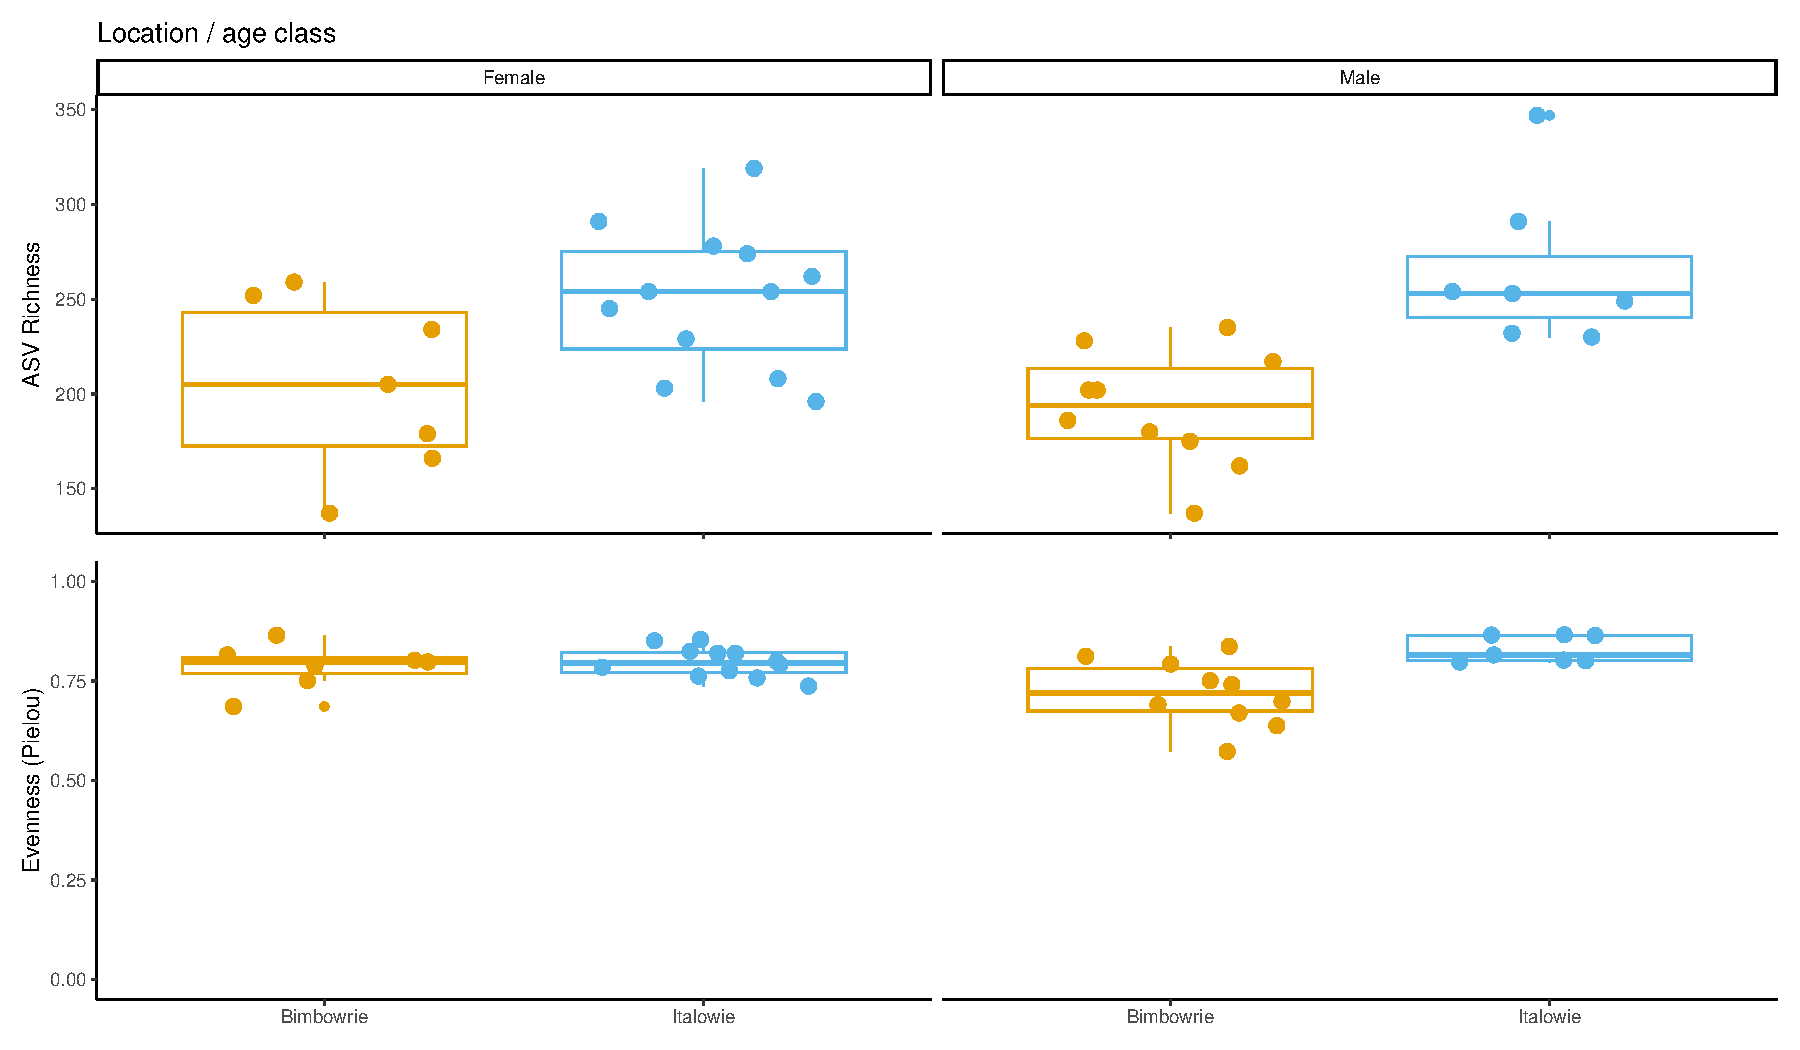
\includegraphics{code_files/figure-pdf/unnamed-chunk-2-1.pdf}

\begin{Shaded}
\begin{Highlighting}[]
\FunctionTok{ggsave}\NormalTok{(}\StringTok{"../figures/noPY\_location\_sex.png"}\NormalTok{, }\AttributeTok{width =} \DecValTok{10}\NormalTok{, }\AttributeTok{height =} \DecValTok{5}\NormalTok{)}
\end{Highlighting}
\end{Shaded}

See slightly lower microbial richness in Bimbowrie compared to Italowie.
Sex does not seem to influence faecal microbiome diversity.

\subsubsection{Alpha diversity (season /
location)}\label{alpha-diversity-season-location}

\begin{Shaded}
\begin{Highlighting}[]
\CommentTok{\#calculate alpha diverisites}
\NormalTok{alpha\_diversity }\OtherTok{\textless{}{-}} \FunctionTok{alpha}\NormalTok{(ps\_adults, }\AttributeTok{index =} \StringTok{"all"}\NormalTok{)}

\CommentTok{\#edit metadata file for plotting}
\NormalTok{metadata }\OtherTok{\textless{}{-}} \FunctionTok{meta}\NormalTok{(ps\_rar)}
\NormalTok{metadata}\SpecialCharTok{$}\NormalTok{name }\OtherTok{\textless{}{-}} \FunctionTok{rownames}\NormalTok{(metadata)}
\NormalTok{alpha\_diversity}\SpecialCharTok{$}\NormalTok{name }\OtherTok{\textless{}{-}} \FunctionTok{rownames}\NormalTok{(alpha\_diversity)}
\NormalTok{alpha\_diversity\_metadata }\OtherTok{\textless{}{-}} \FunctionTok{merge}\NormalTok{(alpha\_diversity, metadata, }\AttributeTok{by =} \StringTok{"name"}\NormalTok{)}

\CommentTok{\#plot}
\NormalTok{a }\OtherTok{\textless{}{-}}\NormalTok{ alpha\_diversity\_metadata }\SpecialCharTok{\%\textgreater{}\%}
  \FunctionTok{ggplot}\NormalTok{(}\FunctionTok{aes}\NormalTok{(}\AttributeTok{x =}\NormalTok{ Location, }\AttributeTok{y =}\NormalTok{ observed, }\AttributeTok{colour =}\NormalTok{ Location)) }\SpecialCharTok{+}
  \FunctionTok{geom\_boxplot}\NormalTok{() }\SpecialCharTok{+}
  \FunctionTok{geom\_jitter}\NormalTok{(}\AttributeTok{size =} \DecValTok{3}\NormalTok{, }\AttributeTok{width =} \FloatTok{0.3}\NormalTok{, }\AttributeTok{height =} \DecValTok{0}\NormalTok{) }\SpecialCharTok{+}
  \FunctionTok{scale\_colour\_manual}\NormalTok{(}\AttributeTok{values =}\NormalTok{ colours) }\SpecialCharTok{+}
  \FunctionTok{theme\_classic}\NormalTok{() }\SpecialCharTok{+}
  \FunctionTok{theme}\NormalTok{(}
    \AttributeTok{axis.title.x =} \FunctionTok{element\_blank}\NormalTok{(),}
    \AttributeTok{legend.position =} \StringTok{"none"}\NormalTok{,}
    \AttributeTok{axis.text.x =} \FunctionTok{element\_blank}\NormalTok{(),}
\NormalTok{    ) }\SpecialCharTok{+}
  \FunctionTok{ylab}\NormalTok{(}\StringTok{"ASV Richness"}\NormalTok{) }\SpecialCharTok{+}
  \FunctionTok{ggtitle}\NormalTok{(}\StringTok{"Location / age class"}\NormalTok{) }\SpecialCharTok{+}
  \FunctionTok{facet\_wrap}\NormalTok{(}\SpecialCharTok{\textasciitilde{}}\NormalTok{Sampling\_trip, }\AttributeTok{nrow =} \DecValTok{1}\NormalTok{)}

\NormalTok{b }\OtherTok{\textless{}{-}}\NormalTok{ alpha\_diversity\_metadata }\SpecialCharTok{\%\textgreater{}\%}
  \FunctionTok{ggplot}\NormalTok{(}\FunctionTok{aes}\NormalTok{(}\AttributeTok{x =}\NormalTok{ Location, }\AttributeTok{y =}\NormalTok{ evenness\_pielou, }\AttributeTok{colour =}\NormalTok{ Location)) }\SpecialCharTok{+}
  \FunctionTok{geom\_boxplot}\NormalTok{() }\SpecialCharTok{+}
  \FunctionTok{geom\_jitter}\NormalTok{(}\AttributeTok{size =} \DecValTok{3}\NormalTok{, }\AttributeTok{width =} \FloatTok{0.3}\NormalTok{, }\AttributeTok{height =} \DecValTok{0}\NormalTok{) }\SpecialCharTok{+}
  \FunctionTok{scale\_colour\_manual}\NormalTok{(}\AttributeTok{values =}\NormalTok{ colours) }\SpecialCharTok{+}
  \FunctionTok{scale\_y\_continuous}\NormalTok{(}\AttributeTok{limits =} \FunctionTok{c}\NormalTok{(}\DecValTok{0}\NormalTok{, }\DecValTok{1}\NormalTok{)) }\SpecialCharTok{+}
  \FunctionTok{theme\_classic}\NormalTok{() }\SpecialCharTok{+}
  \FunctionTok{theme}\NormalTok{(}
    \AttributeTok{axis.title.x =} \FunctionTok{element\_blank}\NormalTok{(),}
    \AttributeTok{legend.position =} \StringTok{"none"}\NormalTok{,}
    \AttributeTok{strip.background =} \FunctionTok{element\_blank}\NormalTok{(),}
    \AttributeTok{strip.text =} \FunctionTok{element\_blank}\NormalTok{()}
\NormalTok{    ) }\SpecialCharTok{+}
  \FunctionTok{ylab}\NormalTok{(}\StringTok{"Evenness (Pielou)"}\NormalTok{) }\SpecialCharTok{+}
  \FunctionTok{facet\_wrap}\NormalTok{(}\SpecialCharTok{\textasciitilde{}}\NormalTok{Sampling\_trip, }\AttributeTok{nrow =} \DecValTok{1}\NormalTok{)}

\CommentTok{\#use patchwork to join figures}
\NormalTok{a }\SpecialCharTok{/}\NormalTok{ b}
\end{Highlighting}
\end{Shaded}

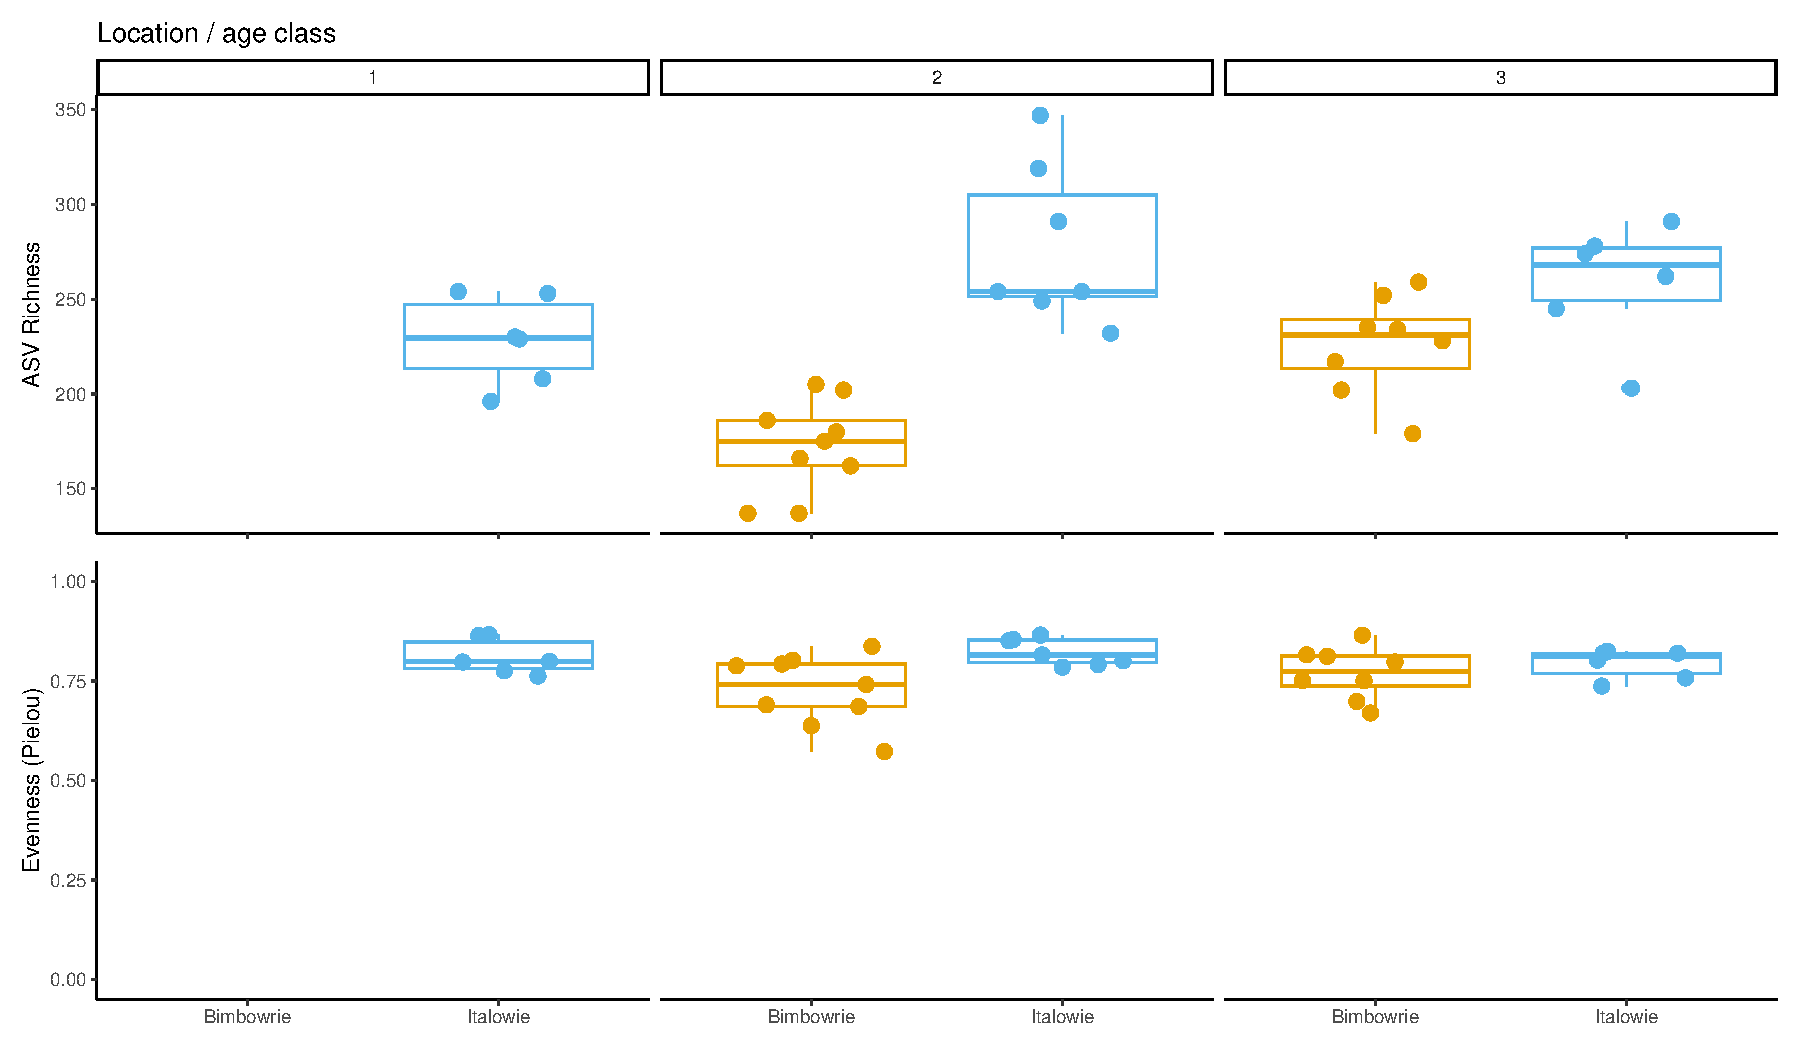
\includegraphics{code_files/figure-pdf/unnamed-chunk-3-1.pdf}

\begin{Shaded}
\begin{Highlighting}[]
\FunctionTok{ggsave}\NormalTok{(}\StringTok{"../figures/noPY\_location\_trip.png"}\NormalTok{, }\AttributeTok{width =} \DecValTok{10}\NormalTok{, }\AttributeTok{height =} \DecValTok{5}\NormalTok{)}
\end{Highlighting}
\end{Shaded}

Can see a moderate difference in ASV richness between season 2/3 for
Bimbowrie, but not for Italowie.

\subsubsection{Alpha diversity stats}\label{alpha-diversity-stats}

\begin{Shaded}
\begin{Highlighting}[]
\FunctionTok{library}\NormalTok{(lme4)}

\CommentTok{\#Refactor Dam\_name to numeric}
\NormalTok{alpha\_diversity\_metadata}\SpecialCharTok{$}\NormalTok{individual\_id }\OtherTok{\textless{}{-}} \FunctionTok{as.numeric}\NormalTok{(}\FunctionTok{factor}\NormalTok{(alpha\_diversity\_metadata}\SpecialCharTok{$}\NormalTok{Dam\_name, }\AttributeTok{levels =} \FunctionTok{unique}\NormalTok{(alpha\_diversity\_metadata}\SpecialCharTok{$}\NormalTok{Dam\_name)))}


\DocumentationTok{\#\#First test if sex influences diversity}
\NormalTok{richness\_sex }\OtherTok{\textless{}{-}} \FunctionTok{lm}\NormalTok{(}\FunctionTok{rank}\NormalTok{(observed) }\SpecialCharTok{\textasciitilde{}}\NormalTok{ Location }\SpecialCharTok{+}\NormalTok{ Animal\_sex }\SpecialCharTok{+}\NormalTok{ (}\DecValTok{1}\SpecialCharTok{|}\NormalTok{individual\_id), }\AttributeTok{data =}\NormalTok{ alpha\_diversity\_metadata)}

\FunctionTok{anova}\NormalTok{(richness\_sex)}
\end{Highlighting}
\end{Shaded}

\begin{verbatim}
Analysis of Variance Table

Response: rank(observed)
           Df  Sum Sq Mean Sq F value    Pr(>F)    
Location    1 1591.61 1591.61 23.0373 3.324e-05 ***
Animal_sex  1    9.98    9.98  0.1445    0.7063    
Residuals  33 2279.91   69.09                      
---
Signif. codes:  0 '***' 0.001 '**' 0.01 '*' 0.05 '.' 0.1 ' ' 1
\end{verbatim}

\begin{Shaded}
\begin{Highlighting}[]
\CommentTok{\#Do the residuals look normally distributed?}
\FunctionTok{hist}\NormalTok{(}\FunctionTok{residuals}\NormalTok{(richness\_sex))}
\end{Highlighting}
\end{Shaded}

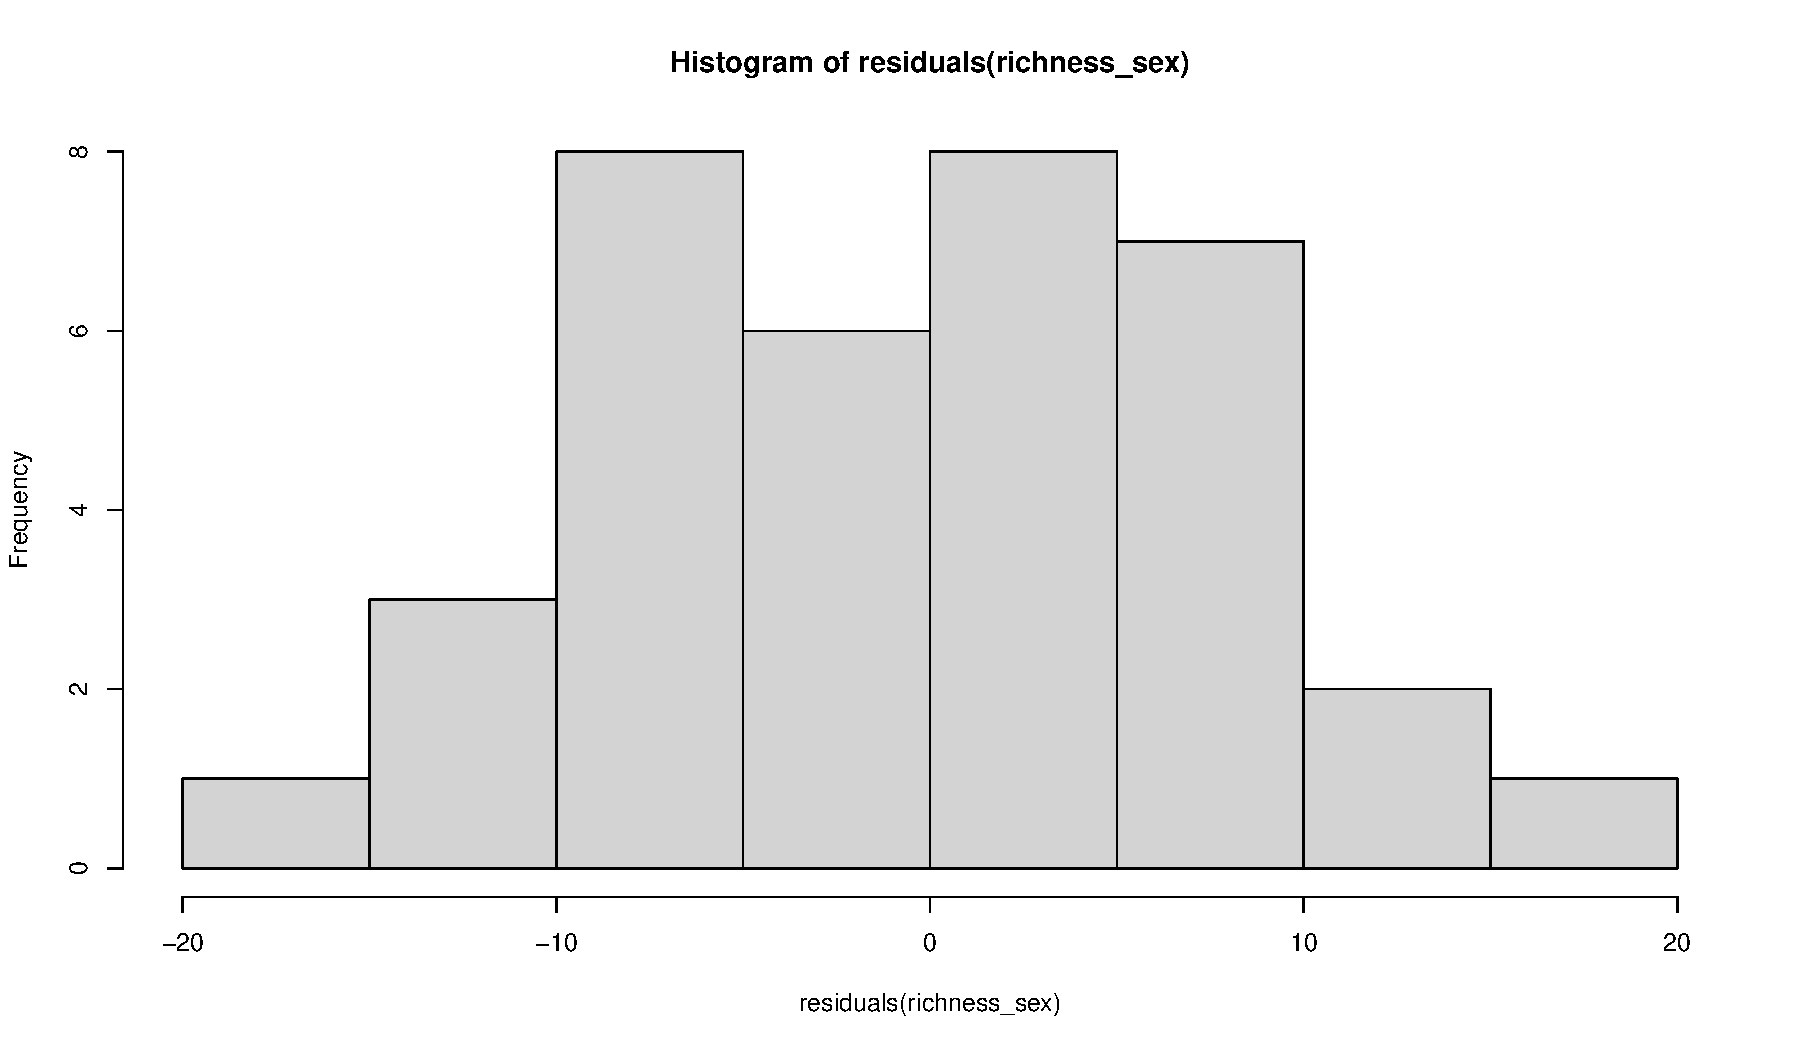
\includegraphics{code_files/figure-pdf/unnamed-chunk-4-1.pdf}

\begin{Shaded}
\begin{Highlighting}[]
\FunctionTok{shapiro.test}\NormalTok{(}\FunctionTok{residuals}\NormalTok{(richness\_sex))}
\end{Highlighting}
\end{Shaded}

\begin{verbatim}

    Shapiro-Wilk normality test

data:  residuals(richness_sex)
W = 0.98413, p-value = 0.8736
\end{verbatim}

\begin{Shaded}
\begin{Highlighting}[]
\DocumentationTok{\#\#Linear model of diversity \textasciitilde{} Location + trip, treating sample as a random effect (some samples come from the same individual)}
\NormalTok{richness }\OtherTok{\textless{}{-}} \FunctionTok{lm}\NormalTok{(}\FunctionTok{rank}\NormalTok{(observed) }\SpecialCharTok{\textasciitilde{}}\NormalTok{ Location }\SpecialCharTok{+}\NormalTok{ Sampling\_trip }\SpecialCharTok{+}\NormalTok{ Location}\SpecialCharTok{:}\NormalTok{Sampling\_trip }\SpecialCharTok{+}\NormalTok{ (}\DecValTok{1}\SpecialCharTok{|}\NormalTok{individual\_id), }\AttributeTok{data =}\NormalTok{ alpha\_diversity\_metadata)}

\FunctionTok{anova}\NormalTok{(richness)}
\end{Highlighting}
\end{Shaded}

\begin{verbatim}
Analysis of Variance Table

Response: rank(observed)
                       Df  Sum Sq Mean Sq F value    Pr(>F)    
Location                1 1591.61 1591.61 37.1323 9.403e-07 ***
Sampling_trip           2  620.36  310.18  7.2366  0.002636 ** 
Location:Sampling_trip  1  340.77  340.77  7.9503  0.008306 ** 
Residuals              31 1328.76   42.86                      
---
Signif. codes:  0 '***' 0.001 '**' 0.01 '*' 0.05 '.' 0.1 ' ' 1
\end{verbatim}

\begin{Shaded}
\begin{Highlighting}[]
\CommentTok{\#Do the residuals look normally distributed?}
\FunctionTok{hist}\NormalTok{(}\FunctionTok{residuals}\NormalTok{(richness))}
\end{Highlighting}
\end{Shaded}

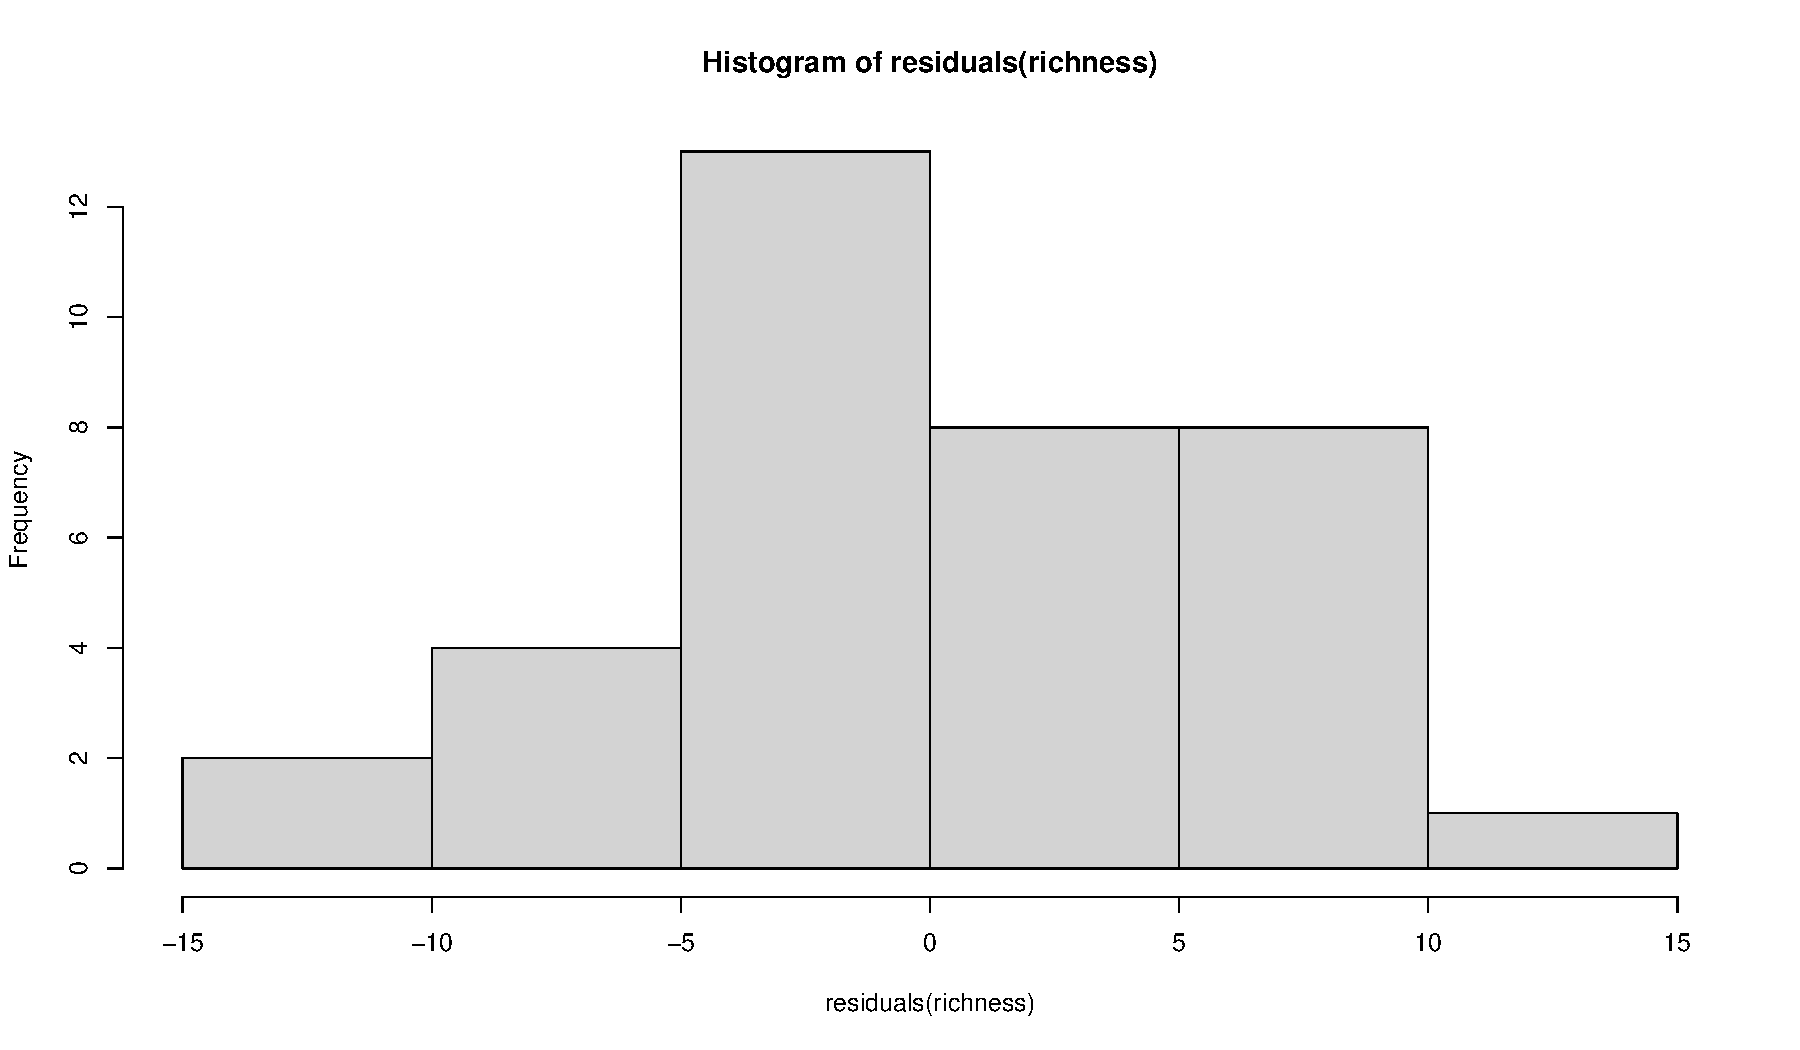
\includegraphics{code_files/figure-pdf/unnamed-chunk-4-2.pdf}

\begin{Shaded}
\begin{Highlighting}[]
\FunctionTok{shapiro.test}\NormalTok{(}\FunctionTok{residuals}\NormalTok{(richness))}
\end{Highlighting}
\end{Shaded}

\begin{verbatim}

    Shapiro-Wilk normality test

data:  residuals(richness)
W = 0.97316, p-value = 0.5181
\end{verbatim}

\begin{Shaded}
\begin{Highlighting}[]
\CommentTok{\#Same for evenness}
\NormalTok{evenness }\OtherTok{\textless{}{-}} \FunctionTok{lm}\NormalTok{(}\FunctionTok{rank}\NormalTok{(evenness\_pielou) }\SpecialCharTok{\textasciitilde{}}\NormalTok{ Location }\SpecialCharTok{+}\NormalTok{ Sampling\_trip }\SpecialCharTok{+}\NormalTok{ Location}\SpecialCharTok{:}\NormalTok{Sampling\_trip }\SpecialCharTok{+}\NormalTok{ (}\DecValTok{1}\SpecialCharTok{|}\NormalTok{individual\_id), }\AttributeTok{data =}\NormalTok{ alpha\_diversity\_metadata)}

\FunctionTok{anova}\NormalTok{(evenness)}
\end{Highlighting}
\end{Shaded}

\begin{verbatim}
Analysis of Variance Table

Response: rank(evenness_pielou)
                       Df  Sum Sq Mean Sq F value Pr(>F)  
Location                1  704.42  704.42  7.2170 0.0115 *
Sampling_trip           2   11.46    5.73  0.0587 0.9431  
Location:Sampling_trip  1  143.33  143.33  1.4684 0.2348  
Residuals              31 3025.79   97.61                 
---
Signif. codes:  0 '***' 0.001 '**' 0.01 '*' 0.05 '.' 0.1 ' ' 1
\end{verbatim}

\begin{Shaded}
\begin{Highlighting}[]
\CommentTok{\#Do the residuals look normally distributed?}
\FunctionTok{hist}\NormalTok{(}\FunctionTok{residuals}\NormalTok{(evenness))}
\end{Highlighting}
\end{Shaded}

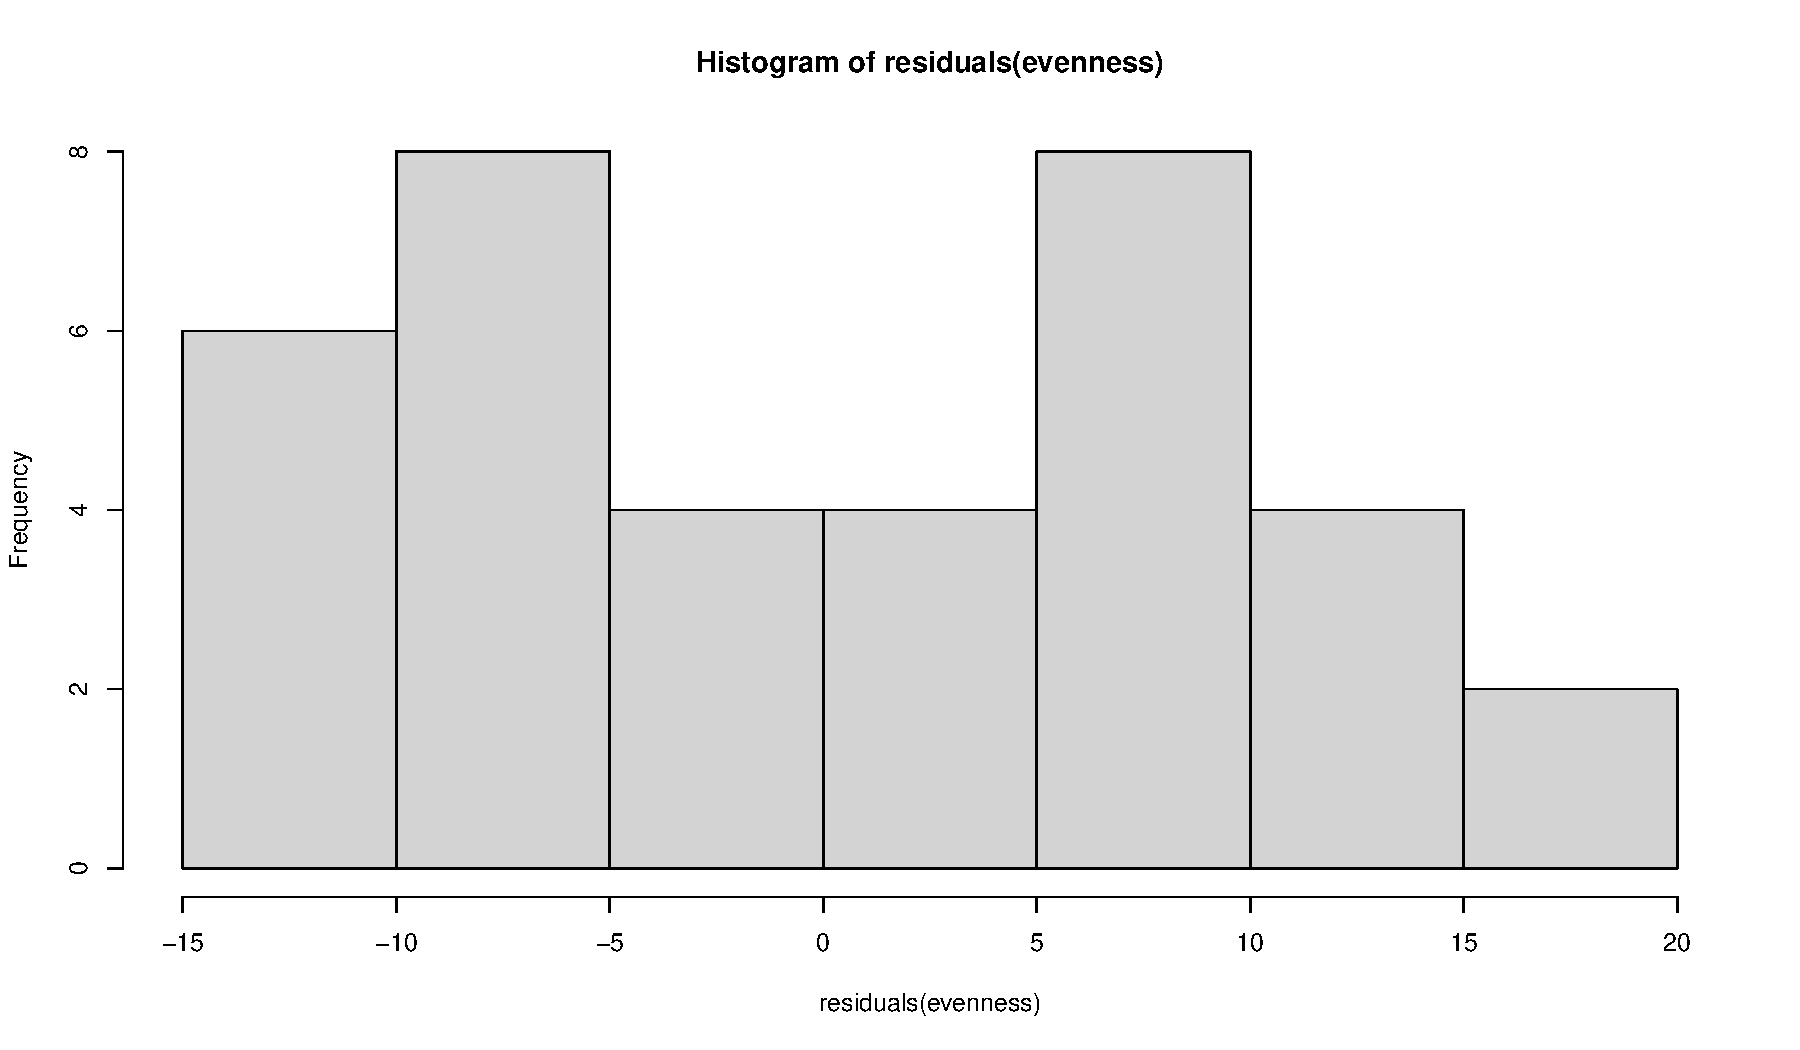
\includegraphics{code_files/figure-pdf/unnamed-chunk-4-3.pdf}

\begin{Shaded}
\begin{Highlighting}[]
\FunctionTok{shapiro.test}\NormalTok{(}\FunctionTok{residuals}\NormalTok{(evenness))}
\end{Highlighting}
\end{Shaded}

\begin{verbatim}

    Shapiro-Wilk normality test

data:  residuals(evenness)
W = 0.93638, p-value = 0.03923
\end{verbatim}

Firstly, sex does not have a statistically significant impact on
microbial diversity (richness).

Next, using the following formula: \textbf{richness \textasciitilde{}
Location + Sampling\_trip + (1\textbar individual\_id)} to look at how
richness is influenced by location and sampling\_trip (with
individual\_id as a random factor to account for some individuals being
sampled across multiple trips).

Location seems to have the largest impact on diversity, though location,
sampling\_trip, and the interaction between sampling\_trip:location are
all statistically significant ( using the arbitrary cutoff of
\emph{p}\textless0.01). Residuals looks normally distributed, and the
Shapiro test suggests normality (\textgreater0.05).

Finally, evenness (with the same formula) paints a different picture.
Only location is statistically significant, though effect size is likely
not biologically relevant, and the \emph{p}-value is high (only 0.011).

In conclusion, sex does not have an observable influence on microbial
richness. Location (strongest), sampling\_trip, and the interaction
between location/sampling trip have a statistically significant
influence on microbial richness. Microbial community evenness however,
does not seem to follow this trend.

\subsubsection{Beta diversity (axes 1/2)}\label{beta-diversity-axes-12}

\begin{Shaded}
\begin{Highlighting}[]
\FunctionTok{library}\NormalTok{(vegan)}

\CommentTok{\#Beta diversity}
\NormalTok{unweighted\_unifrac }\OtherTok{\textless{}{-}} \FunctionTok{ordinate}\NormalTok{(ps\_adults, }
                               \AttributeTok{method =} \StringTok{"PCoA"}\NormalTok{, }
                               \AttributeTok{distance =} \StringTok{"unifrac"}\NormalTok{, }\AttributeTok{weighted=}\NormalTok{F)}

\NormalTok{weighted\_unifrac }\OtherTok{\textless{}{-}} \FunctionTok{ordinate}\NormalTok{(ps\_adults, }
                               \AttributeTok{method =} \StringTok{"PCoA"}\NormalTok{, }
                               \AttributeTok{distance =} \StringTok{"unifrac"}\NormalTok{, }\AttributeTok{weighted=}\NormalTok{T)}

\CommentTok{\#Unweighted}
\NormalTok{uw }\OtherTok{\textless{}{-}} \FunctionTok{plot\_ordination}\NormalTok{(}\AttributeTok{physeq =}\NormalTok{ ps\_adults,}
                \AttributeTok{ordination =}\NormalTok{ unweighted\_unifrac,}
                \AttributeTok{color =} \StringTok{"Location"}\NormalTok{,}
                \AttributeTok{shape =} \StringTok{"Animal\_sex"}\NormalTok{,}
                \AttributeTok{axes =} \FunctionTok{c}\NormalTok{(}\DecValTok{1}\NormalTok{, }\DecValTok{2}\NormalTok{)) }\SpecialCharTok{+}
  \FunctionTok{geom\_point}\NormalTok{(}\AttributeTok{size =} \DecValTok{4}\NormalTok{) }\SpecialCharTok{+}
  \FunctionTok{theme\_minimal}\NormalTok{() }\SpecialCharTok{+}
  \FunctionTok{scale\_colour\_manual}\NormalTok{(}\AttributeTok{values =}\NormalTok{ colours) }\SpecialCharTok{+}
  \FunctionTok{theme\_classic}\NormalTok{() }\SpecialCharTok{+}
  \FunctionTok{ggtitle}\NormalTok{(}\StringTok{"A) Unweighted UniFrac"}\NormalTok{) }\SpecialCharTok{+}
  \FunctionTok{theme}\NormalTok{(}
    \AttributeTok{legend.position =} \StringTok{"none"}\NormalTok{,}
    \AttributeTok{legend.title =} \FunctionTok{element\_blank}\NormalTok{()}
\NormalTok{    ) }

\CommentTok{\#Weighted}
\NormalTok{w }\OtherTok{\textless{}{-}} \FunctionTok{plot\_ordination}\NormalTok{(}\AttributeTok{physeq =}\NormalTok{ ps\_adults,}
                \AttributeTok{ordination =}\NormalTok{ weighted\_unifrac,}
                \AttributeTok{color =} \StringTok{"Location"}\NormalTok{,}
                \AttributeTok{shape =} \StringTok{"Animal\_sex"}\NormalTok{,}
                \AttributeTok{axes =} \FunctionTok{c}\NormalTok{(}\DecValTok{1}\NormalTok{, }\DecValTok{2}\NormalTok{)) }\SpecialCharTok{+}
  \FunctionTok{geom\_point}\NormalTok{(}\AttributeTok{size =} \DecValTok{4}\NormalTok{) }\SpecialCharTok{+}
  \FunctionTok{theme\_minimal}\NormalTok{() }\SpecialCharTok{+}
  \FunctionTok{scale\_colour\_manual}\NormalTok{(}\AttributeTok{values =}\NormalTok{ colours) }\SpecialCharTok{+}
  \FunctionTok{theme\_classic}\NormalTok{() }\SpecialCharTok{+}
  \FunctionTok{ggtitle}\NormalTok{(}\StringTok{"B) Weighted UniFrac"}\NormalTok{) }\SpecialCharTok{+}
  \FunctionTok{theme}\NormalTok{(}
    \AttributeTok{legend.position =} \StringTok{"top"}\NormalTok{,}
    \AttributeTok{legend.title =} \FunctionTok{element\_blank}\NormalTok{(),}
    \AttributeTok{axis.text =} \FunctionTok{element\_text}\NormalTok{(}\AttributeTok{size =} \DecValTok{14}\NormalTok{),}
    \AttributeTok{axis.title =} \FunctionTok{element\_text}\NormalTok{(}\AttributeTok{size =} \DecValTok{16}\NormalTok{),}
    \AttributeTok{legend.text =} \FunctionTok{element\_text}\NormalTok{(}\AttributeTok{size =} \DecValTok{16}\NormalTok{),}
\NormalTok{    ) }

\NormalTok{combined }\OtherTok{\textless{}{-}}\NormalTok{ uw }\SpecialCharTok{/}\NormalTok{ w}
\NormalTok{combined}
\end{Highlighting}
\end{Shaded}

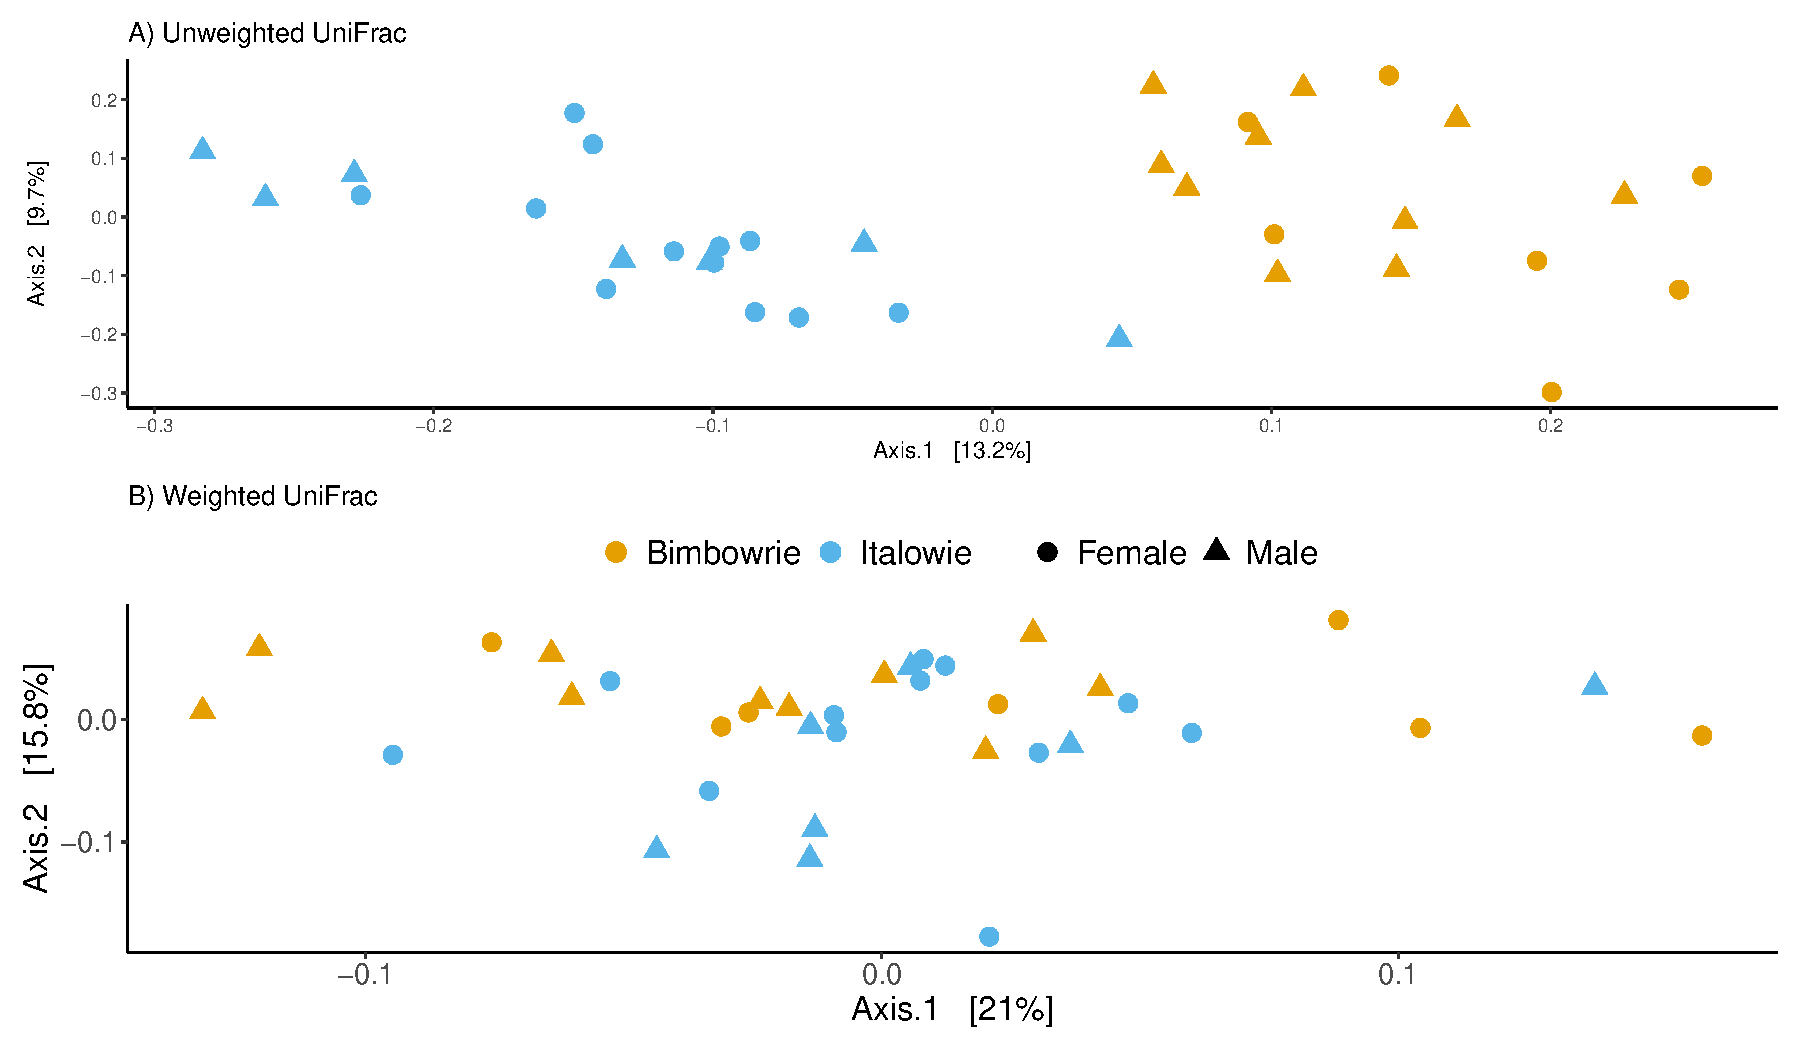
\includegraphics{code_files/figure-pdf/unnamed-chunk-5-1.pdf}

\begin{Shaded}
\begin{Highlighting}[]
\FunctionTok{ggsave}\NormalTok{(}\StringTok{"../figures/beta\_div\_sex\_1\_2.png"}\NormalTok{, }\AttributeTok{plot =}\NormalTok{ combined, }\AttributeTok{height =} \DecValTok{10}\NormalTok{, }\AttributeTok{width =} \DecValTok{10}\NormalTok{)}


\DocumentationTok{\#\# Adonis (similar to PERMANOVA) test}
\CommentTok{\#refactor metadata}
\NormalTok{md\_adults }\OtherTok{\textless{}{-}} \FunctionTok{as}\NormalTok{(}\FunctionTok{sample\_data}\NormalTok{(ps\_adults), }\StringTok{"data.frame"}\NormalTok{)}

\NormalTok{md\_adults}\SpecialCharTok{$}\NormalTok{individual\_id }\OtherTok{\textless{}{-}} \FunctionTok{as.numeric}\NormalTok{(}\FunctionTok{factor}\NormalTok{(md\_adults}\SpecialCharTok{$}\NormalTok{Dam\_name, }
                                             \AttributeTok{levels =} \FunctionTok{unique}\NormalTok{(md\_adults}\SpecialCharTok{$}\NormalTok{Dam\_name)))}

\CommentTok{\#Run adonis: location + sampling\_trip + (1|individual\_id) with 9999 permutations}
\NormalTok{uw\_adonis }\OtherTok{\textless{}{-}} \FunctionTok{adonis2}\NormalTok{(}\FunctionTok{distance}\NormalTok{(ps\_adults, }\AttributeTok{method=}\StringTok{"unifrac"}\NormalTok{) }\SpecialCharTok{\textasciitilde{}}\NormalTok{ Location }\SpecialCharTok{+}\NormalTok{ Animal\_sex }\SpecialCharTok{+}\NormalTok{ Sampling\_trip }\SpecialCharTok{+}\NormalTok{ (}\DecValTok{1}\SpecialCharTok{|}\NormalTok{individual\_id), }\AttributeTok{data =}\NormalTok{ md\_adults, }\AttributeTok{permutations =} \DecValTok{9999}\NormalTok{)}

\NormalTok{uw\_adonis}
\end{Highlighting}
\end{Shaded}

\begin{verbatim}
Permutation test for adonis under reduced model
Terms added sequentially (first to last)
Permutation: free
Number of permutations: 9999

adonis2(formula = distance(ps_adults, method = "unifrac") ~ Location + Animal_sex + Sampling_trip + (1 | individual_id), data = md_adults, permutations = 9999)
              Df SumOfSqs      R2      F Pr(>F)    
Location       1   0.7387 0.11745 4.7187 0.0001 ***
Animal_sex     1   0.1505 0.02394 0.9617 0.5053    
Sampling_trip  2   0.5473 0.08702 1.7481 0.0002 ***
Residual      31   4.8529 0.77159                  
Total         35   6.2894 1.00000                  
---
Signif. codes:  0 '***' 0.001 '**' 0.01 '*' 0.05 '.' 0.1 ' ' 1
\end{verbatim}

\begin{Shaded}
\begin{Highlighting}[]
\CommentTok{\#Check for homogenaeity multivariate dispersion with betadisper}
\NormalTok{location }\OtherTok{\textless{}{-}}\NormalTok{ md\_adults[[}\StringTok{"Location"}\NormalTok{]]}
\NormalTok{uw\_disp }\OtherTok{\textless{}{-}} \FunctionTok{betadisper}\NormalTok{(}\FunctionTok{distance}\NormalTok{(ps\_adults, }\AttributeTok{method=}\StringTok{"unifrac"}\NormalTok{), }\AttributeTok{group =}\NormalTok{ location)}

\FunctionTok{anova}\NormalTok{(uw\_disp)}
\end{Highlighting}
\end{Shaded}

\begin{verbatim}
Analysis of Variance Table

Response: Distances
          Df   Sum Sq   Mean Sq F value Pr(>F)
Groups     1 0.002642 0.0026416  1.4668 0.2342
Residuals 34 0.061232 0.0018009               
\end{verbatim}

\begin{Shaded}
\begin{Highlighting}[]
\CommentTok{\#plots for homoegenaeity}

\FunctionTok{plot}\NormalTok{(uw\_disp)}
\end{Highlighting}
\end{Shaded}

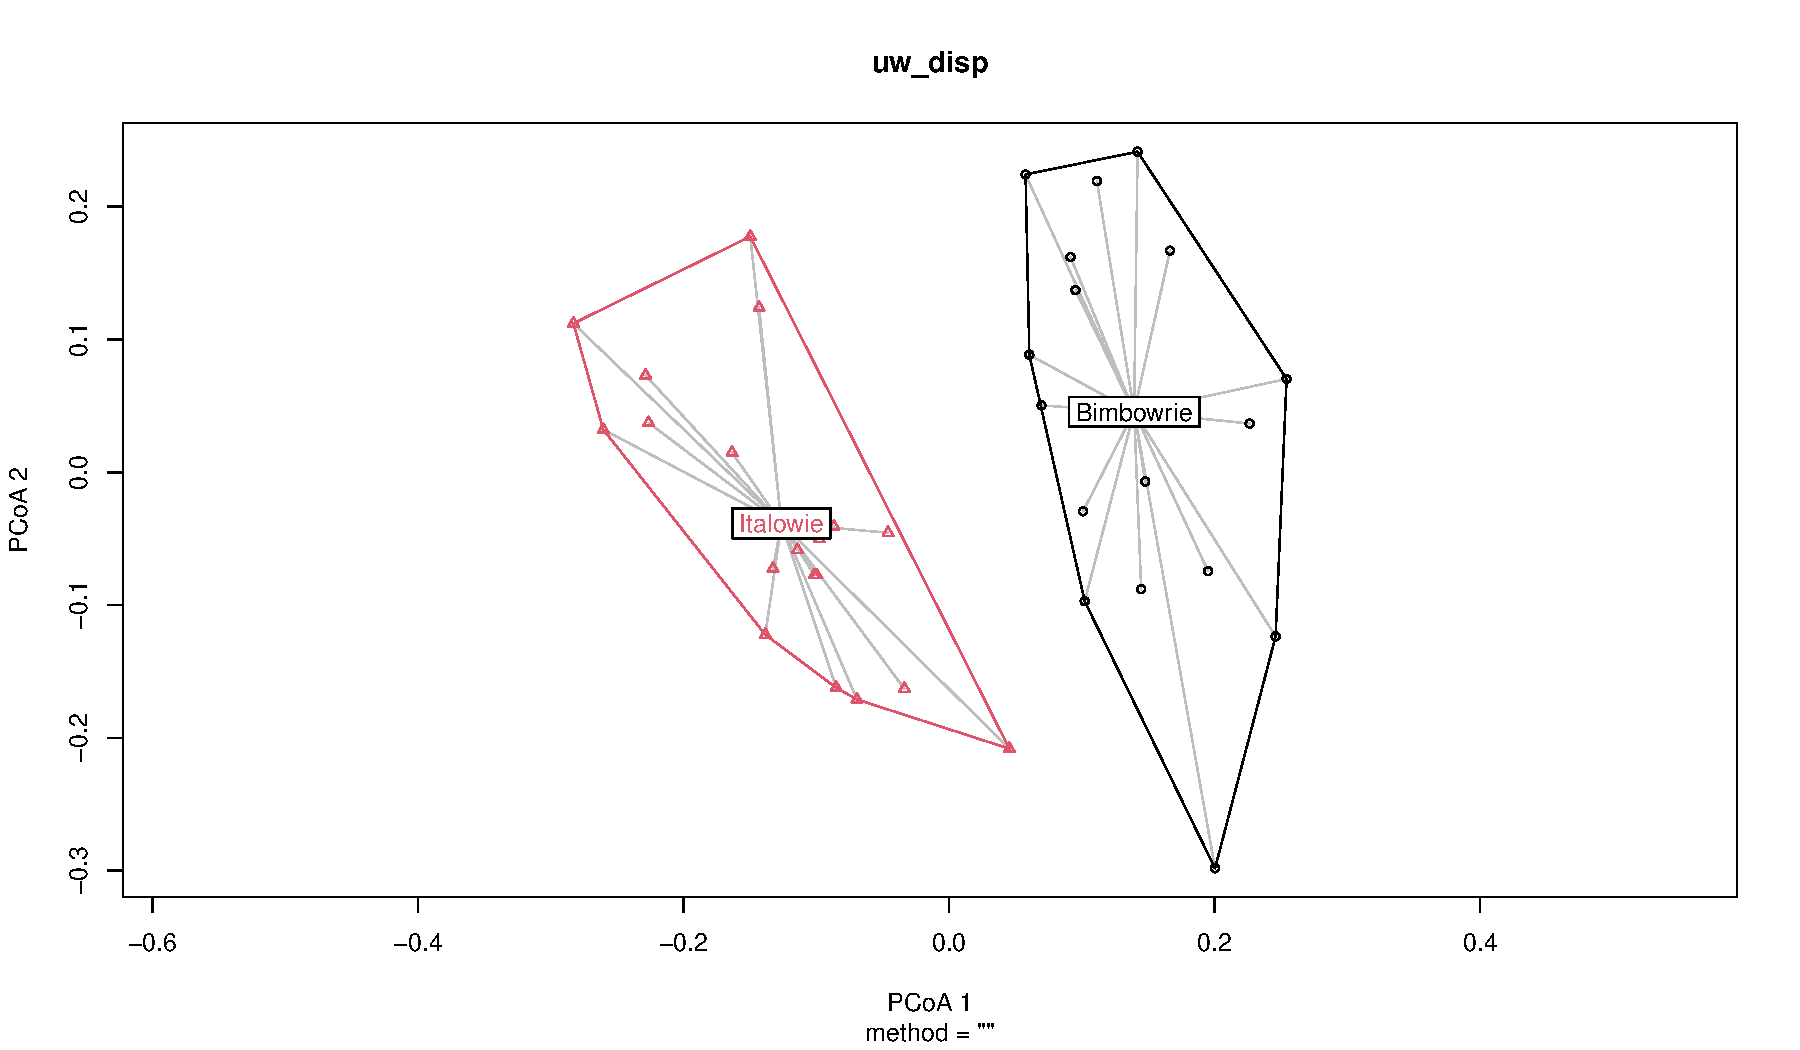
\includegraphics{code_files/figure-pdf/unnamed-chunk-5-2.pdf}

\begin{Shaded}
\begin{Highlighting}[]
\FunctionTok{boxplot}\NormalTok{(uw\_disp)}
\end{Highlighting}
\end{Shaded}

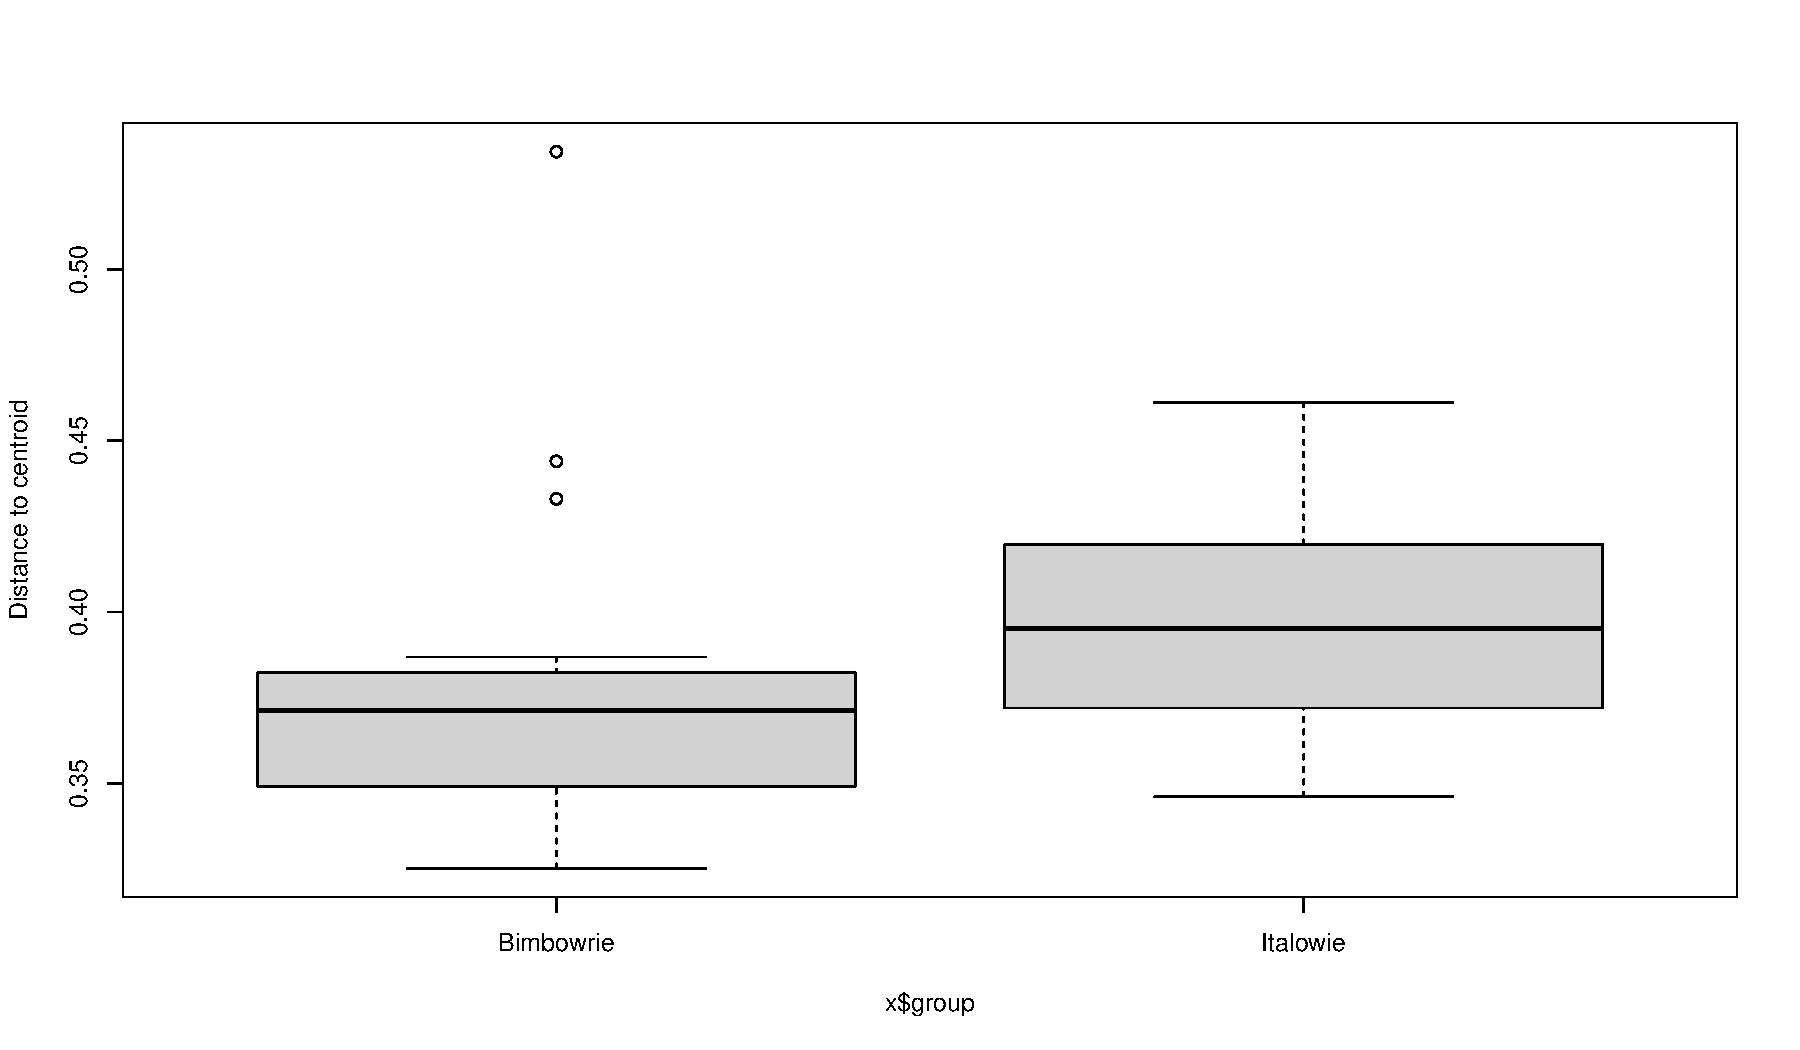
\includegraphics{code_files/figure-pdf/unnamed-chunk-5-3.pdf}

\begin{Shaded}
\begin{Highlighting}[]
\CommentTok{\#Tukey HSD}
\NormalTok{uw\_disp\_HSD }\OtherTok{\textless{}{-}} \FunctionTok{TukeyHSD}\NormalTok{(uw\_disp)}
\FunctionTok{plot}\NormalTok{(uw\_disp\_HSD)}
\end{Highlighting}
\end{Shaded}

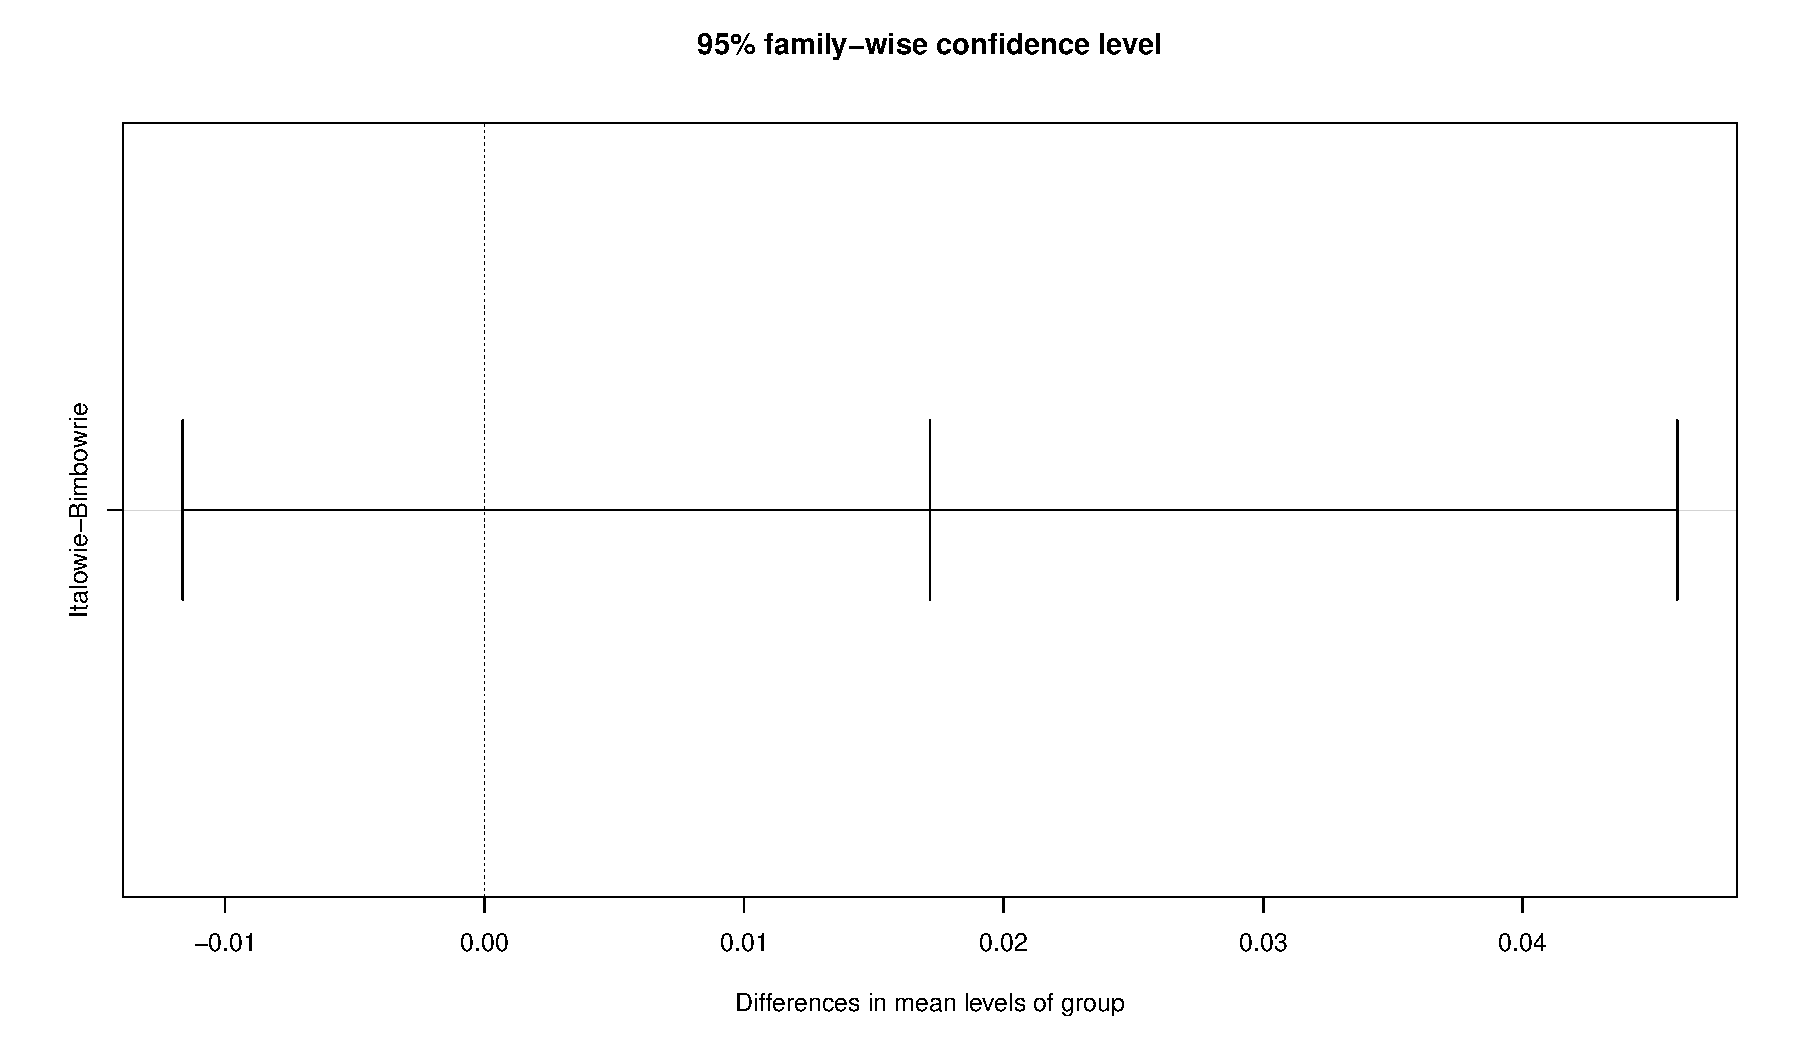
\includegraphics{code_files/figure-pdf/unnamed-chunk-5-4.pdf}

\begin{Shaded}
\begin{Highlighting}[]
\DocumentationTok{\#\#Now same for weighted unifrac}
\NormalTok{w\_adonis }\OtherTok{\textless{}{-}} \FunctionTok{adonis2}\NormalTok{(}\FunctionTok{distance}\NormalTok{(ps\_adults, }\AttributeTok{method=}\StringTok{"wunifrac"}\NormalTok{) }\SpecialCharTok{\textasciitilde{}}\NormalTok{ Location }\SpecialCharTok{+}\NormalTok{ Animal\_sex }\SpecialCharTok{+}\NormalTok{ Sampling\_trip }\SpecialCharTok{+}\NormalTok{ (}\DecValTok{1}\SpecialCharTok{|}\NormalTok{individual\_id), }\AttributeTok{data =}\NormalTok{ md\_adults, }\AttributeTok{permutations =} \DecValTok{9999}\NormalTok{)}

\NormalTok{w\_adonis}
\end{Highlighting}
\end{Shaded}

\begin{verbatim}
Permutation test for adonis under reduced model
Terms added sequentially (first to last)
Permutation: free
Number of permutations: 9999

adonis2(formula = distance(ps_adults, method = "wunifrac") ~ Location + Animal_sex + Sampling_trip + (1 | individual_id), data = md_adults, permutations = 9999)
              Df SumOfSqs      R2      F Pr(>F)   
Location       1  0.04927 0.07470 2.7777 0.0013 **
Animal_sex     1  0.01384 0.02098 0.7801 0.6989   
Sampling_trip  2  0.04661 0.07068 1.3141 0.1275   
Residual      31  0.54983 0.83365                 
Total         35  0.65955 1.00000                 
---
Signif. codes:  0 '***' 0.001 '**' 0.01 '*' 0.05 '.' 0.1 ' ' 1
\end{verbatim}

\begin{Shaded}
\begin{Highlighting}[]
\CommentTok{\#Check for homogenaeity multivariate dispersion with betadisper}
\NormalTok{location }\OtherTok{\textless{}{-}}\NormalTok{ md\_adults[[}\StringTok{"Location"}\NormalTok{]]}
\NormalTok{w\_disp }\OtherTok{\textless{}{-}} \FunctionTok{betadisper}\NormalTok{(}\FunctionTok{distance}\NormalTok{(ps\_adults, }\AttributeTok{method=}\StringTok{"wunifrac"}\NormalTok{), }\AttributeTok{group =}\NormalTok{ location)}

\FunctionTok{anova}\NormalTok{(w\_disp)}
\end{Highlighting}
\end{Shaded}

\begin{verbatim}
Analysis of Variance Table

Response: Distances
          Df   Sum Sq   Mean Sq F value Pr(>F)
Groups     1 0.001860 0.0018595    1.22 0.2771
Residuals 34 0.051821 0.0015241               
\end{verbatim}

\begin{Shaded}
\begin{Highlighting}[]
\CommentTok{\#plots for homoegenaeity}

\FunctionTok{plot}\NormalTok{(w\_disp)}
\end{Highlighting}
\end{Shaded}

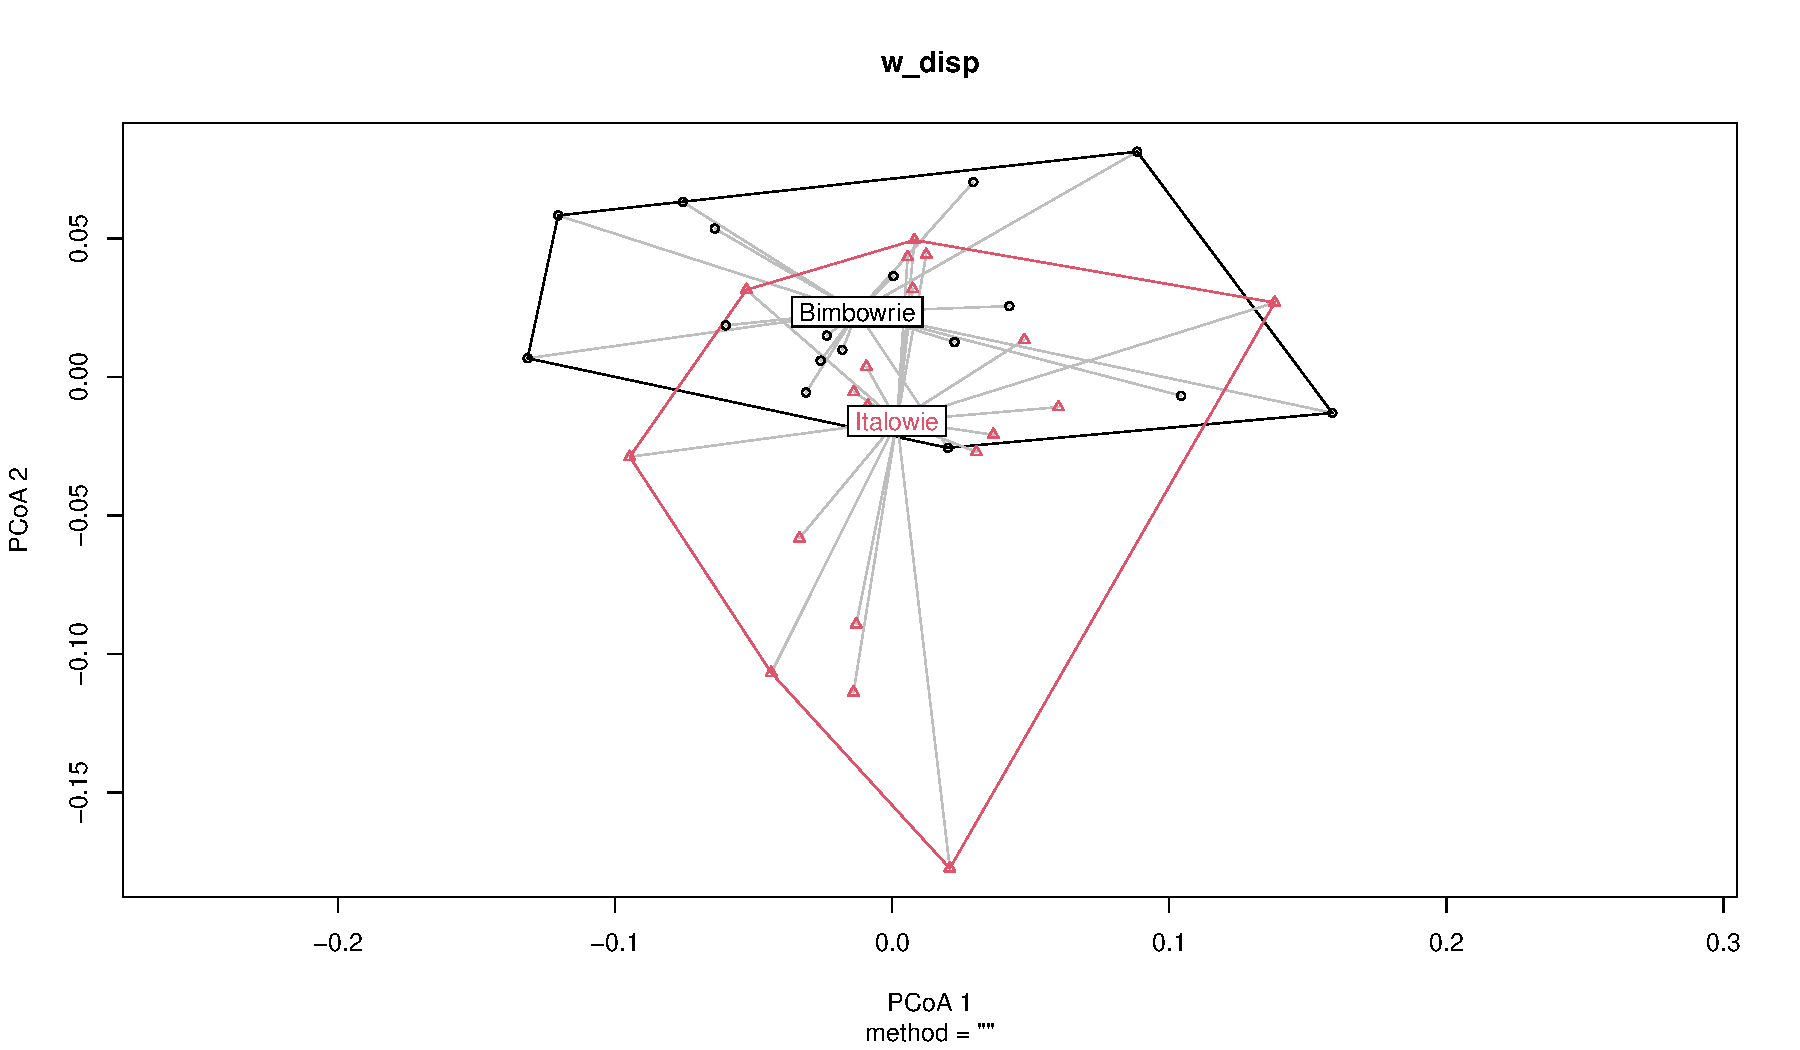
\includegraphics{code_files/figure-pdf/unnamed-chunk-5-5.pdf}

\begin{Shaded}
\begin{Highlighting}[]
\FunctionTok{boxplot}\NormalTok{(w\_disp)}
\end{Highlighting}
\end{Shaded}

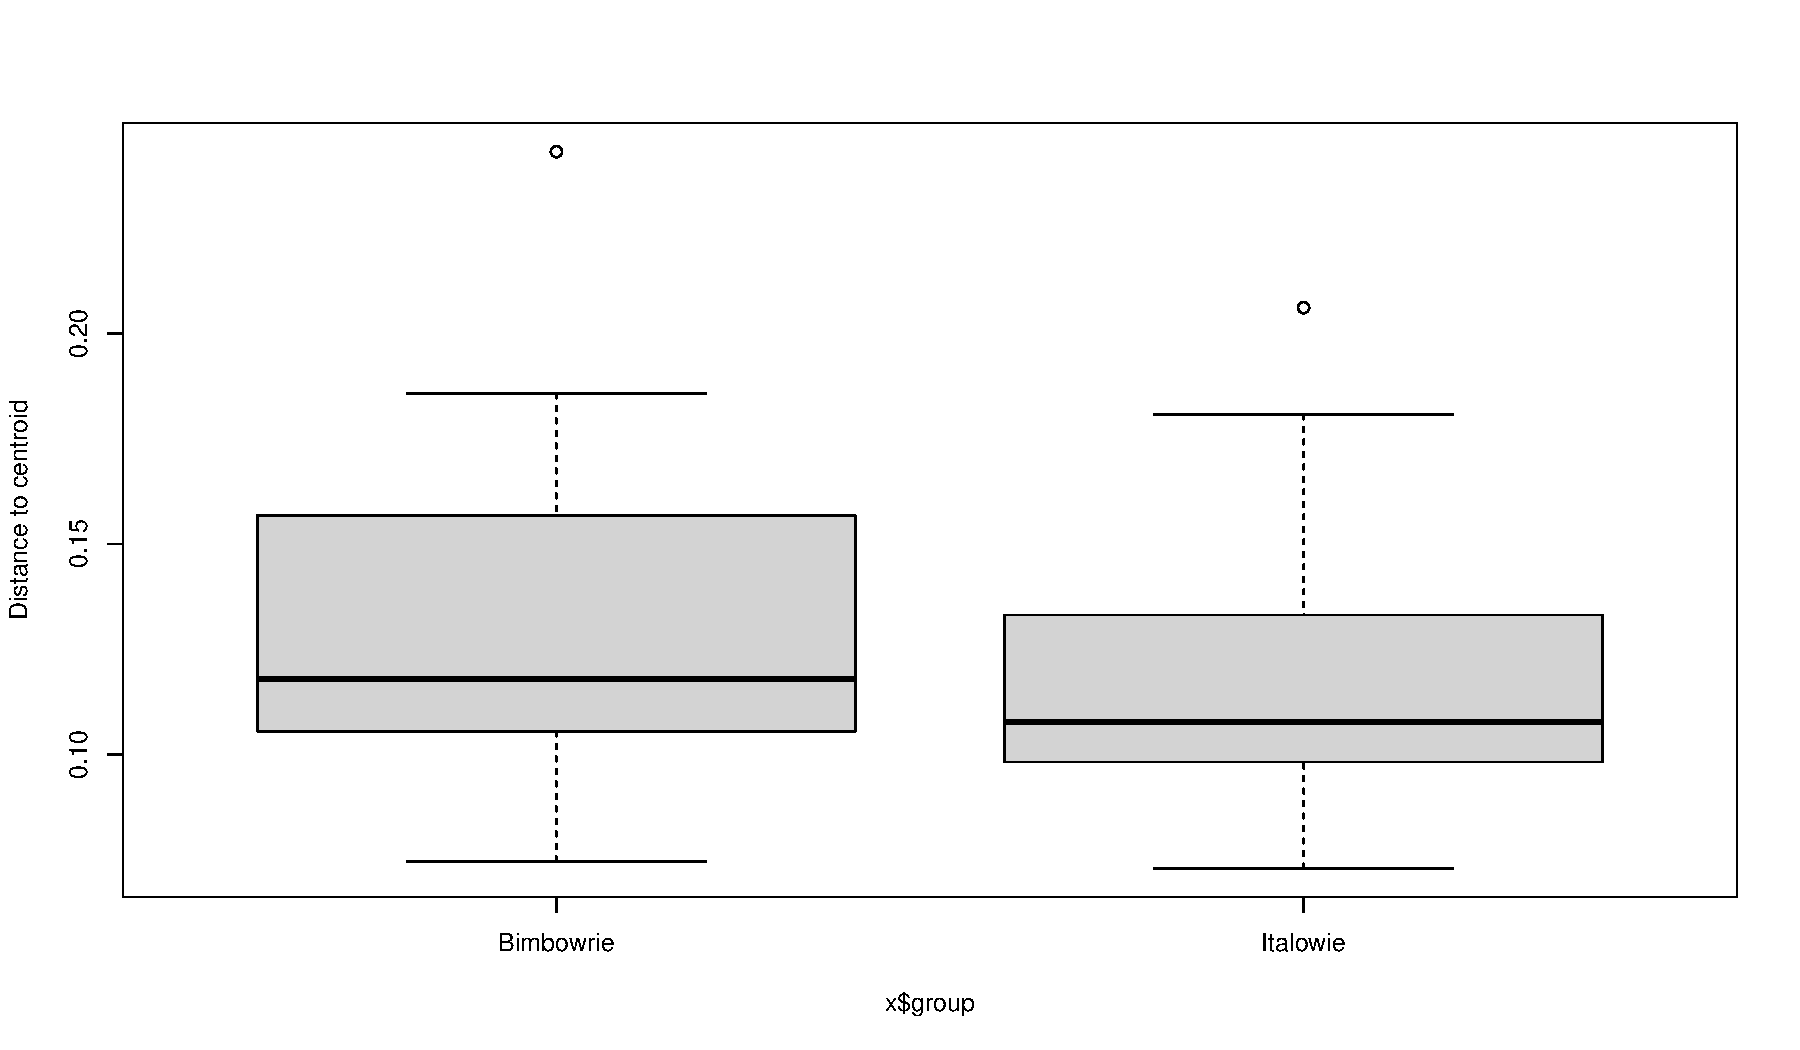
\includegraphics{code_files/figure-pdf/unnamed-chunk-5-6.pdf}

\begin{Shaded}
\begin{Highlighting}[]
\CommentTok{\#Tukey HSD}
\NormalTok{w\_disp\_HSD }\OtherTok{\textless{}{-}} \FunctionTok{TukeyHSD}\NormalTok{(w\_disp)}
\FunctionTok{plot}\NormalTok{(w\_disp\_HSD)}
\end{Highlighting}
\end{Shaded}

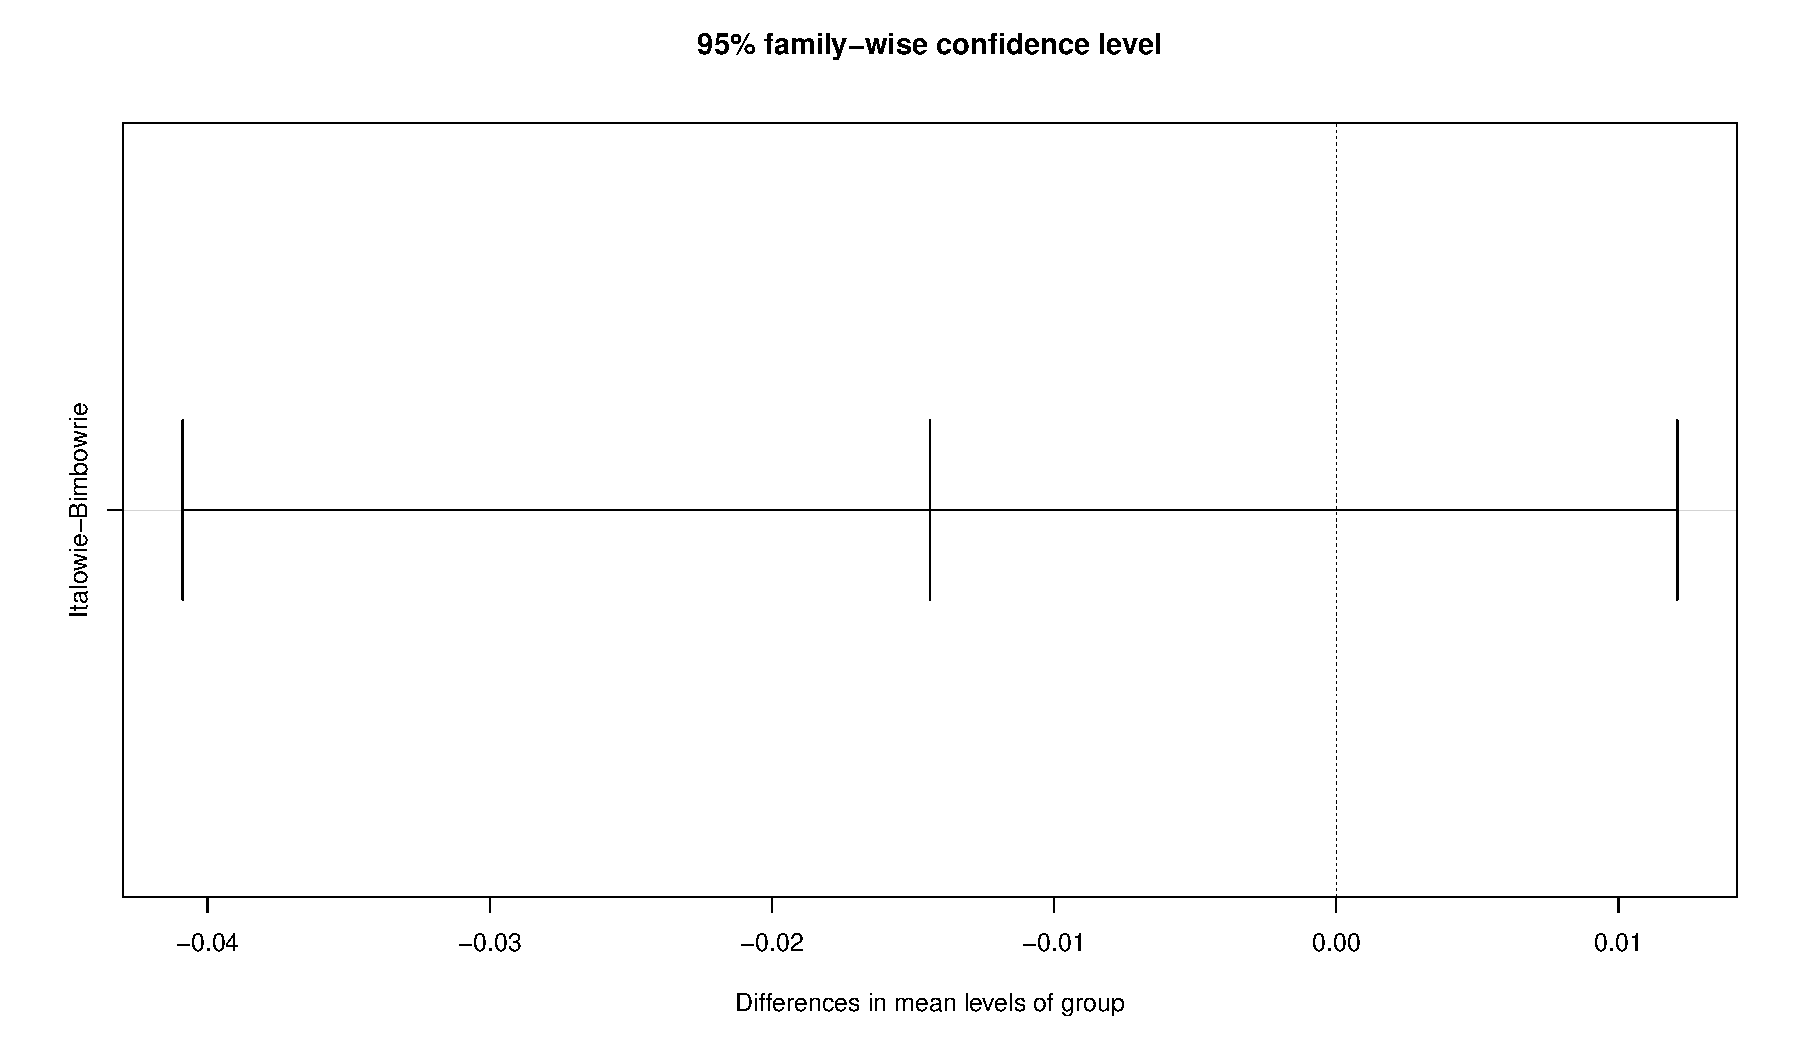
\includegraphics{code_files/figure-pdf/unnamed-chunk-5-7.pdf}

Use Adonis (PERMANOVA-like) to test for statistically significant
influences of metadata on microbial composition. I'll use a similar
formula to the alpha diversity tests above:

\texttt{Location\ +\ Animal\_sex\ +\ Sampling\_trip\ +\ (1\textbar{}individual\_id)}

\textbf{Unweighted UniFrac\\
}Again, sex has no statistically significant (observable) impact on
microbial composition. Location explains more variation (R2 = 0.117)
compared to sampling\_trip (R2 = 0.087). Both are statistically
significant. Still quite a lot of residual variation (R2 = 0.77). I then
test for homogeneity of variance between groups (assumption of
PERMANOVA) using betadisper. Plots and Tukey's HSD suggest no meaningful
variation in homogeneity between groups.

\textbf{Weighted UniFrac\\
}Similar results to Unweighted UniFrac, except only location is
statistically significant, and variation explained is lower (R2 =
0.074). Assumptions regarding homogeneity also seem fine as above.

\subsubsection{Beta diversity (axes 1/3)}\label{beta-diversity-axes-13}

\begin{Shaded}
\begin{Highlighting}[]
\CommentTok{\#Beta diversity}
\NormalTok{unweighted\_unifrac }\OtherTok{\textless{}{-}} \FunctionTok{ordinate}\NormalTok{(ps\_adults, }
                               \AttributeTok{method =} \StringTok{"PCoA"}\NormalTok{, }
                               \AttributeTok{distance =} \StringTok{"unifrac"}\NormalTok{, }\AttributeTok{weighted=}\NormalTok{F)}

\NormalTok{weighted\_unifrac }\OtherTok{\textless{}{-}} \FunctionTok{ordinate}\NormalTok{(ps\_adults, }
                               \AttributeTok{method =} \StringTok{"PCoA"}\NormalTok{, }
                               \AttributeTok{distance =} \StringTok{"unifrac"}\NormalTok{, }\AttributeTok{weighted=}\NormalTok{T)}

\CommentTok{\#Unweighted}
\NormalTok{uw }\OtherTok{\textless{}{-}} \FunctionTok{plot\_ordination}\NormalTok{(}\AttributeTok{physeq =}\NormalTok{ ps\_adults,}
                \AttributeTok{ordination =}\NormalTok{ unweighted\_unifrac,}
                \AttributeTok{color =} \StringTok{"Location"}\NormalTok{,}
                \AttributeTok{shape =} \StringTok{"Animal\_sex"}\NormalTok{,}
                \AttributeTok{axes =} \FunctionTok{c}\NormalTok{(}\DecValTok{1}\NormalTok{, }\DecValTok{3}\NormalTok{)) }\SpecialCharTok{+}
  \FunctionTok{geom\_point}\NormalTok{(}\AttributeTok{size =} \DecValTok{4}\NormalTok{) }\SpecialCharTok{+}
  \FunctionTok{theme\_minimal}\NormalTok{() }\SpecialCharTok{+}
  \FunctionTok{scale\_colour\_manual}\NormalTok{(}\AttributeTok{values =}\NormalTok{ colours) }\SpecialCharTok{+}
  \FunctionTok{theme\_classic}\NormalTok{() }\SpecialCharTok{+}
  \FunctionTok{ggtitle}\NormalTok{(}\StringTok{"A) Unweighted UniFrac"}\NormalTok{) }\SpecialCharTok{+}
  \FunctionTok{theme}\NormalTok{(}
    \AttributeTok{legend.position =} \StringTok{"none"}\NormalTok{,}
    \AttributeTok{legend.title =} \FunctionTok{element\_blank}\NormalTok{()}
\NormalTok{    ) }

\CommentTok{\#Weighted}
\NormalTok{w }\OtherTok{\textless{}{-}} \FunctionTok{plot\_ordination}\NormalTok{(}\AttributeTok{physeq =}\NormalTok{ ps\_adults,}
                \AttributeTok{ordination =}\NormalTok{ weighted\_unifrac,}
                \AttributeTok{color =} \StringTok{"Location"}\NormalTok{,}
                \AttributeTok{shape =} \StringTok{"Animal\_sex"}\NormalTok{,}
                \AttributeTok{axes =} \FunctionTok{c}\NormalTok{(}\DecValTok{1}\NormalTok{, }\DecValTok{3}\NormalTok{)) }\SpecialCharTok{+}
  \FunctionTok{geom\_point}\NormalTok{(}\AttributeTok{size =} \DecValTok{4}\NormalTok{) }\SpecialCharTok{+}
  \FunctionTok{theme\_minimal}\NormalTok{() }\SpecialCharTok{+}
  \FunctionTok{scale\_colour\_manual}\NormalTok{(}\AttributeTok{values =}\NormalTok{ colours) }\SpecialCharTok{+}
  \FunctionTok{theme\_classic}\NormalTok{() }\SpecialCharTok{+}
  \FunctionTok{ggtitle}\NormalTok{(}\StringTok{"B) Weighted UniFrac"}\NormalTok{) }\SpecialCharTok{+}
  \FunctionTok{theme}\NormalTok{(}
    \AttributeTok{legend.position =} \StringTok{"top"}\NormalTok{,}
    \AttributeTok{legend.title =} \FunctionTok{element\_blank}\NormalTok{(),}
    \AttributeTok{axis.text =} \FunctionTok{element\_text}\NormalTok{(}\AttributeTok{size =} \DecValTok{14}\NormalTok{),}
    \AttributeTok{axis.title =} \FunctionTok{element\_text}\NormalTok{(}\AttributeTok{size =} \DecValTok{16}\NormalTok{),}
    \AttributeTok{legend.text =} \FunctionTok{element\_text}\NormalTok{(}\AttributeTok{size =} \DecValTok{16}\NormalTok{),}
\NormalTok{    ) }

\NormalTok{combined }\OtherTok{\textless{}{-}}\NormalTok{ uw }\SpecialCharTok{/}\NormalTok{ w}
\NormalTok{combined}
\end{Highlighting}
\end{Shaded}

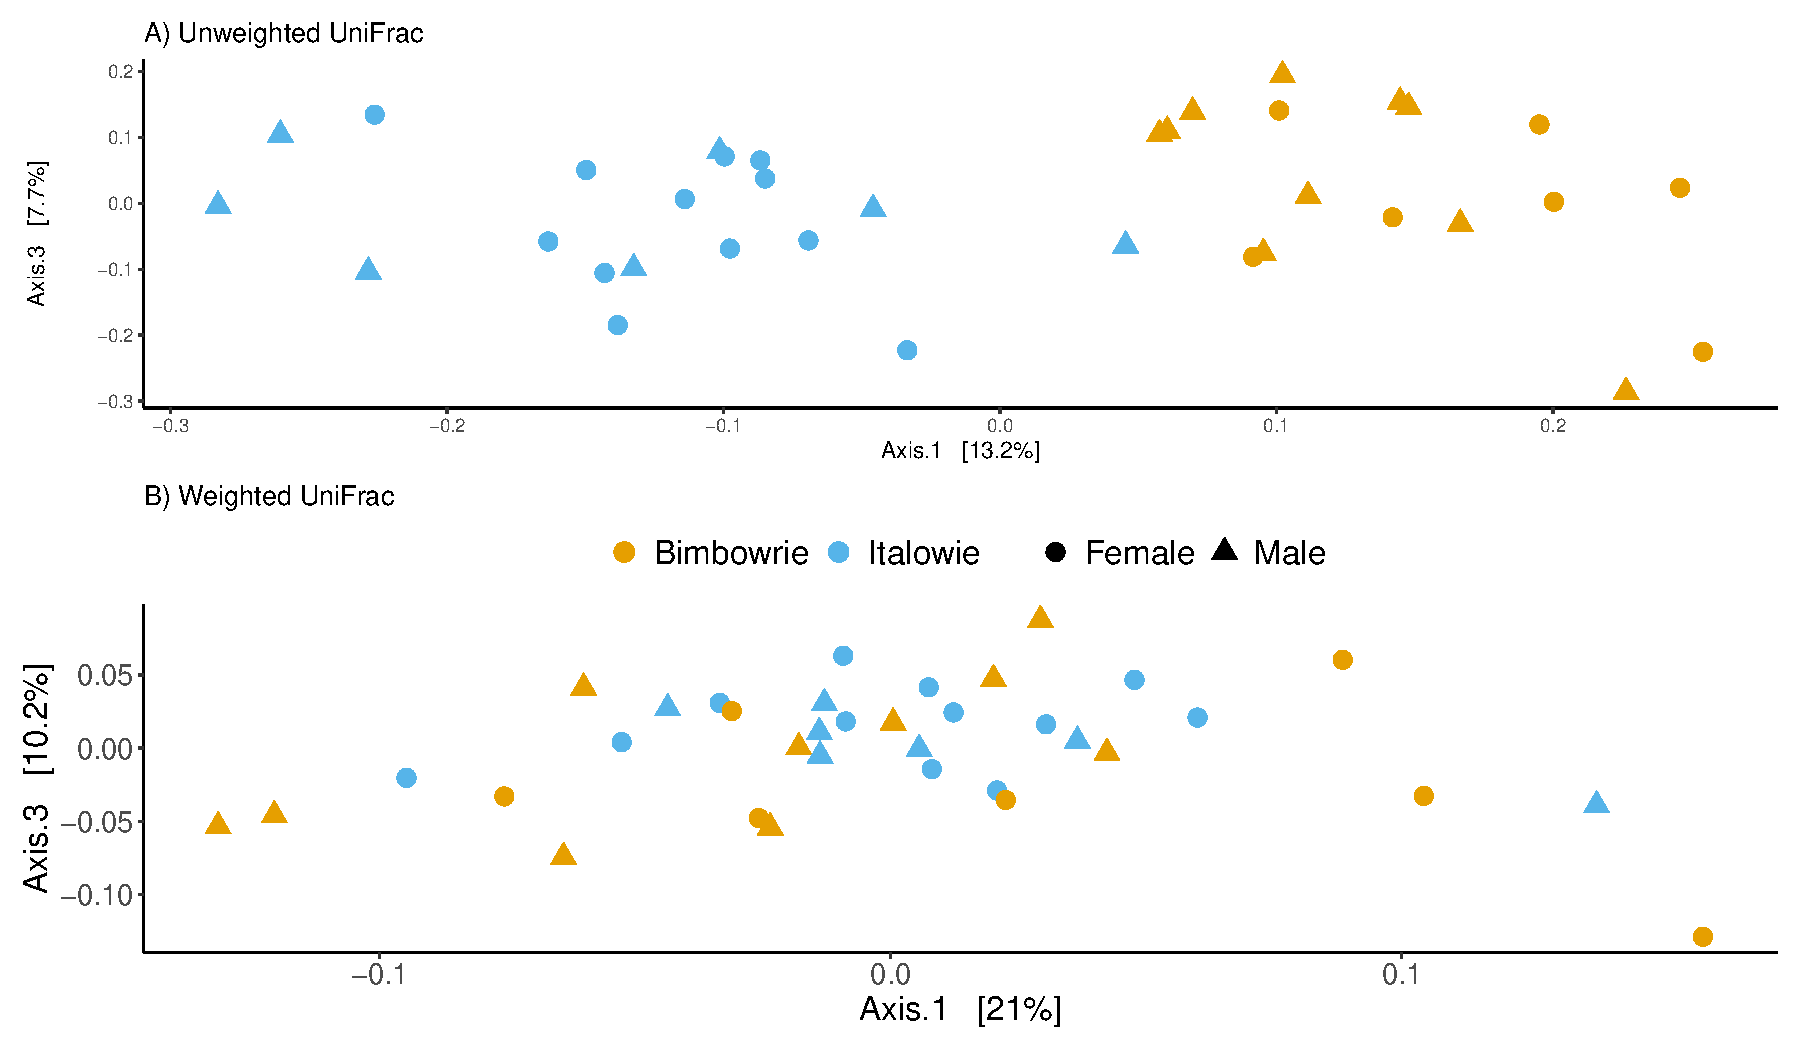
\includegraphics{code_files/figure-pdf/unnamed-chunk-6-1.pdf}

\begin{Shaded}
\begin{Highlighting}[]
\FunctionTok{ggsave}\NormalTok{(}\StringTok{"../figures/beta\_div\_sex\_1\_3.png"}\NormalTok{, }\AttributeTok{plot =}\NormalTok{ combined, }\AttributeTok{height =} \DecValTok{10}\NormalTok{, }\AttributeTok{width =} \DecValTok{10}\NormalTok{)}
\end{Highlighting}
\end{Shaded}

Likewise for axes 1/3. (Didn't do tests here, but can if needed).

\subsubsection{Beta diversity (separate ordinations for
locations)}\label{beta-diversity-separate-ordinations-for-locations}

Given that location seems to drive most variation, lets try splitting
the ordinations then looking at season.

\begin{Shaded}
\begin{Highlighting}[]
\CommentTok{\#Split table}
\NormalTok{ps\_bimb }\OtherTok{\textless{}{-}} \FunctionTok{subset\_samples}\NormalTok{(ps\_adults, Location }\SpecialCharTok{==} \StringTok{"Bimbowrie"}\NormalTok{)}
\NormalTok{ps\_ital }\OtherTok{\textless{}{-}} \FunctionTok{subset\_samples}\NormalTok{(ps\_adults, Location }\SpecialCharTok{==} \StringTok{"Italowie"}\NormalTok{)}

\CommentTok{\#Beta diversity}
\NormalTok{unweighted\_unifrac }\OtherTok{\textless{}{-}} \FunctionTok{ordinate}\NormalTok{(ps\_bimb, }
                               \AttributeTok{method =} \StringTok{"PCoA"}\NormalTok{, }
                               \AttributeTok{distance =} \StringTok{"unifrac"}\NormalTok{, }\AttributeTok{weighted=}\NormalTok{F)}

\NormalTok{weighted\_unifrac }\OtherTok{\textless{}{-}} \FunctionTok{ordinate}\NormalTok{(ps\_bimb, }
                               \AttributeTok{method =} \StringTok{"PCoA"}\NormalTok{, }
                               \AttributeTok{distance =} \StringTok{"unifrac"}\NormalTok{, }\AttributeTok{weighted=}\NormalTok{T)}

\CommentTok{\#Bimbowrie}
\CommentTok{\#Unweighted}
\NormalTok{uw }\OtherTok{\textless{}{-}} \FunctionTok{plot\_ordination}\NormalTok{(}\AttributeTok{physeq =}\NormalTok{ ps\_bimb,}
                \AttributeTok{ordination =}\NormalTok{ unweighted\_unifrac,}
                \AttributeTok{color =} \StringTok{"season"}\NormalTok{,}
\CommentTok{\#                shape = "Dam\_with\_PY",}
                \AttributeTok{axes =} \FunctionTok{c}\NormalTok{(}\DecValTok{1}\NormalTok{, }\DecValTok{2}\NormalTok{)) }\SpecialCharTok{+}
  \FunctionTok{geom\_point}\NormalTok{(}\AttributeTok{size =} \DecValTok{4}\NormalTok{) }\SpecialCharTok{+}
  \FunctionTok{theme\_minimal}\NormalTok{() }\SpecialCharTok{+}
  \FunctionTok{scale\_colour\_manual}\NormalTok{(}\AttributeTok{values =}\NormalTok{ colours) }\SpecialCharTok{+}
  \FunctionTok{theme\_classic}\NormalTok{() }\SpecialCharTok{+}
  \FunctionTok{ggtitle}\NormalTok{(}\StringTok{"A) Unweighted UniFrac"}\NormalTok{) }\SpecialCharTok{+}
  \FunctionTok{theme}\NormalTok{(}
    \AttributeTok{legend.position =} \StringTok{"none"}\NormalTok{,}
    \AttributeTok{legend.title =} \FunctionTok{element\_blank}\NormalTok{()}
\NormalTok{    ) }

\CommentTok{\#Weighted}
\NormalTok{w }\OtherTok{\textless{}{-}} \FunctionTok{plot\_ordination}\NormalTok{(}\AttributeTok{physeq =}\NormalTok{ ps\_bimb,}
                \AttributeTok{ordination =}\NormalTok{ weighted\_unifrac,}
                \AttributeTok{color =} \StringTok{"season"}\NormalTok{,}
\CommentTok{\#                shape = "Dam\_with\_PY",}
                \AttributeTok{axes =} \FunctionTok{c}\NormalTok{(}\DecValTok{1}\NormalTok{, }\DecValTok{2}\NormalTok{)) }\SpecialCharTok{+}
  \FunctionTok{geom\_point}\NormalTok{(}\AttributeTok{size =} \DecValTok{4}\NormalTok{) }\SpecialCharTok{+}
  \FunctionTok{theme\_minimal}\NormalTok{() }\SpecialCharTok{+}
  \FunctionTok{scale\_colour\_manual}\NormalTok{(}\AttributeTok{values =}\NormalTok{ colours) }\SpecialCharTok{+}
  \FunctionTok{theme\_classic}\NormalTok{() }\SpecialCharTok{+}
  \FunctionTok{ggtitle}\NormalTok{(}\StringTok{"B) Weighted UniFrac"}\NormalTok{) }\SpecialCharTok{+}
  \FunctionTok{theme}\NormalTok{(}
    \AttributeTok{legend.position =} \StringTok{"top"}\NormalTok{,}
    \AttributeTok{legend.title =} \FunctionTok{element\_blank}\NormalTok{(),}
    \AttributeTok{axis.text =} \FunctionTok{element\_text}\NormalTok{(}\AttributeTok{size =} \DecValTok{14}\NormalTok{),}
    \AttributeTok{axis.title =} \FunctionTok{element\_text}\NormalTok{(}\AttributeTok{size =} \DecValTok{16}\NormalTok{),}
    \AttributeTok{legend.text =} \FunctionTok{element\_text}\NormalTok{(}\AttributeTok{size =} \DecValTok{16}\NormalTok{),}
\NormalTok{    ) }

\NormalTok{bimb\_combined }\OtherTok{\textless{}{-}}\NormalTok{ uw }\SpecialCharTok{/}\NormalTok{ w}
\NormalTok{bimb\_combined}
\end{Highlighting}
\end{Shaded}

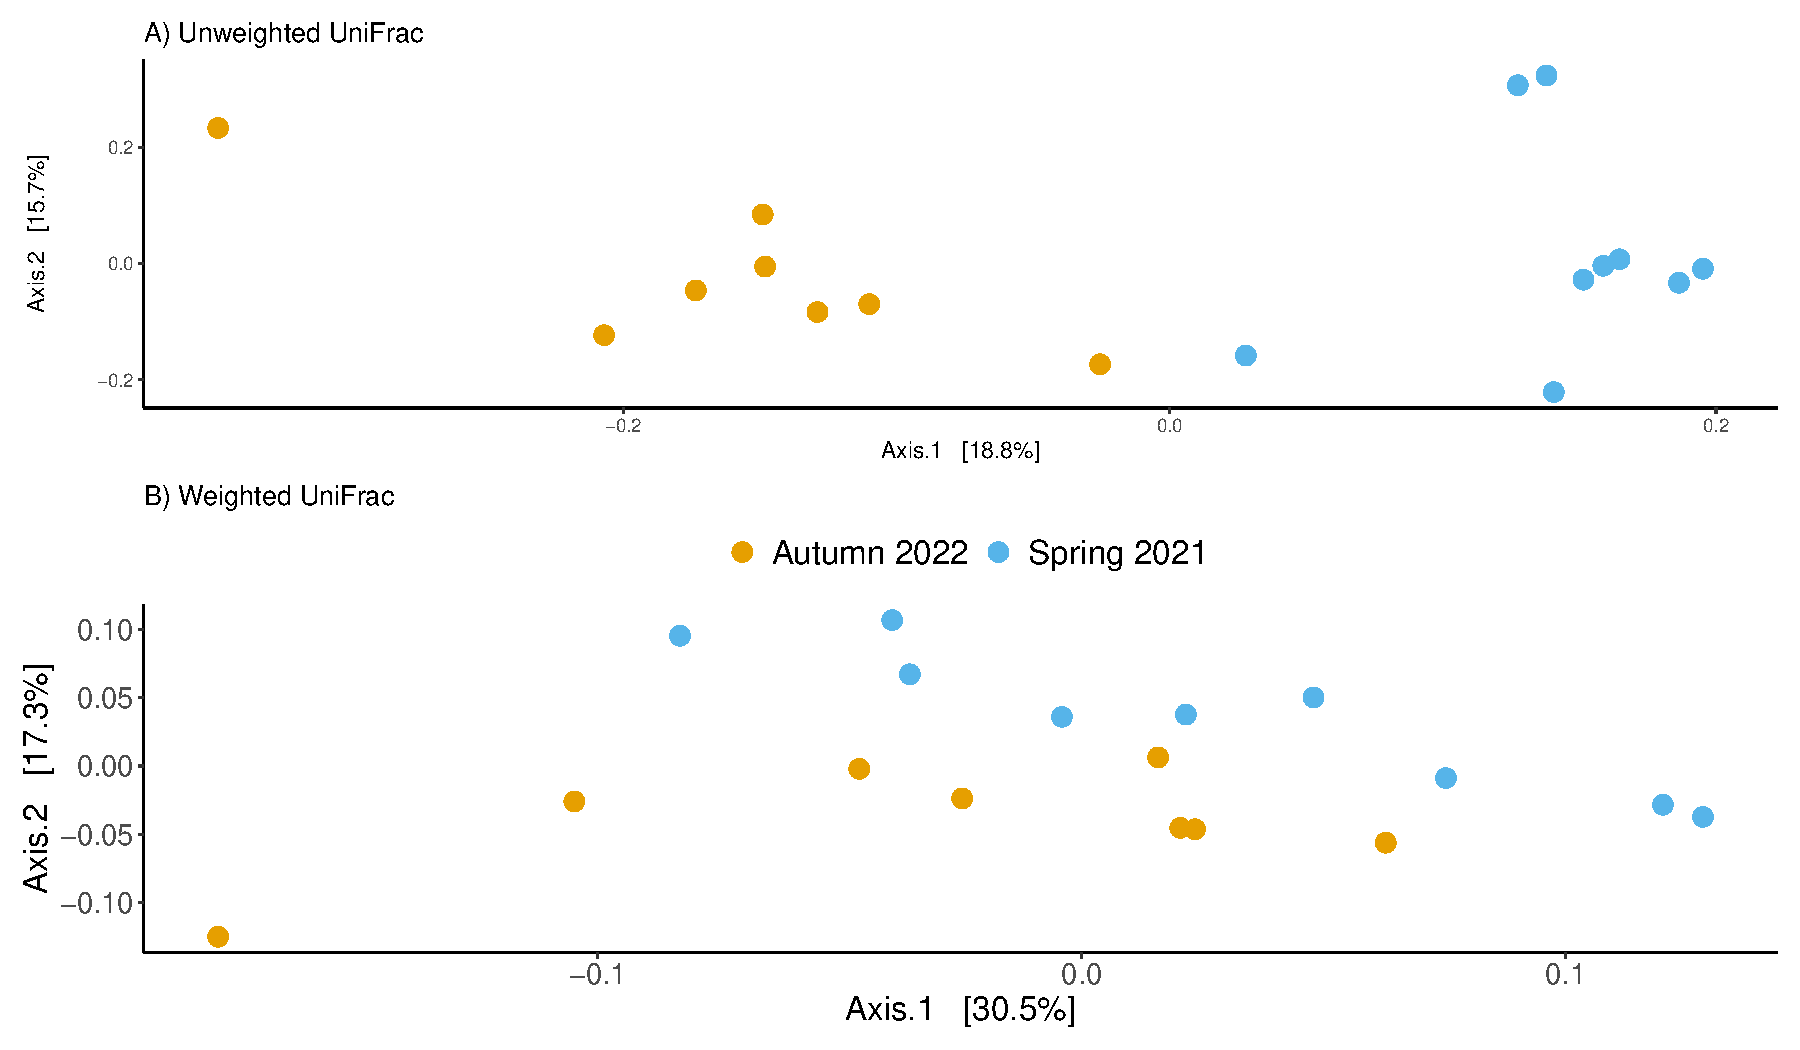
\includegraphics{code_files/figure-pdf/unnamed-chunk-7-1.pdf}

\begin{Shaded}
\begin{Highlighting}[]
\FunctionTok{ggsave}\NormalTok{(}\StringTok{"../figures/beta\_div\_bimb\_1\_2.png"}\NormalTok{, }\AttributeTok{plot =}\NormalTok{ bimb\_combined, }\AttributeTok{height =} \DecValTok{10}\NormalTok{, }\AttributeTok{width =} \DecValTok{10}\NormalTok{)}




\CommentTok{\#Italowie}

\NormalTok{unweighted\_unifrac }\OtherTok{\textless{}{-}} \FunctionTok{ordinate}\NormalTok{(ps\_ital, }
                               \AttributeTok{method =} \StringTok{"PCoA"}\NormalTok{, }
                               \AttributeTok{distance =} \StringTok{"unifrac"}\NormalTok{, }\AttributeTok{weighted=}\NormalTok{F)}

\NormalTok{weighted\_unifrac }\OtherTok{\textless{}{-}} \FunctionTok{ordinate}\NormalTok{(ps\_ital, }
                               \AttributeTok{method =} \StringTok{"PCoA"}\NormalTok{, }
                               \AttributeTok{distance =} \StringTok{"unifrac"}\NormalTok{, }\AttributeTok{weighted=}\NormalTok{T)}
\CommentTok{\#Unweighted}
\NormalTok{uw }\OtherTok{\textless{}{-}} \FunctionTok{plot\_ordination}\NormalTok{(}\AttributeTok{physeq =}\NormalTok{ ps\_ital,}
                \AttributeTok{ordination =}\NormalTok{ unweighted\_unifrac,}
                \AttributeTok{color =} \StringTok{"season"}\NormalTok{,}
                \AttributeTok{axes =} \FunctionTok{c}\NormalTok{(}\DecValTok{1}\NormalTok{, }\DecValTok{2}\NormalTok{)) }\SpecialCharTok{+}
  \FunctionTok{geom\_point}\NormalTok{(}\AttributeTok{size =} \DecValTok{4}\NormalTok{) }\SpecialCharTok{+}
  \FunctionTok{theme\_minimal}\NormalTok{() }\SpecialCharTok{+}
  \FunctionTok{scale\_colour\_manual}\NormalTok{(}\AttributeTok{values =}\NormalTok{ colours) }\SpecialCharTok{+}
  \FunctionTok{theme\_classic}\NormalTok{() }\SpecialCharTok{+}
  \FunctionTok{ggtitle}\NormalTok{(}\StringTok{"A) Unweighted UniFrac"}\NormalTok{) }\SpecialCharTok{+}
  \FunctionTok{theme}\NormalTok{(}
    \AttributeTok{legend.position =} \StringTok{"none"}\NormalTok{,}
    \AttributeTok{legend.title =} \FunctionTok{element\_blank}\NormalTok{()}
\NormalTok{    ) }

\CommentTok{\#Weighted}
\NormalTok{w }\OtherTok{\textless{}{-}} \FunctionTok{plot\_ordination}\NormalTok{(}\AttributeTok{physeq =}\NormalTok{ ps\_ital,}
                \AttributeTok{ordination =}\NormalTok{ weighted\_unifrac,}
                \AttributeTok{color =} \StringTok{"season"}\NormalTok{,}
                \AttributeTok{axes =} \FunctionTok{c}\NormalTok{(}\DecValTok{1}\NormalTok{, }\DecValTok{2}\NormalTok{)) }\SpecialCharTok{+}
  \FunctionTok{geom\_point}\NormalTok{(}\AttributeTok{size =} \DecValTok{4}\NormalTok{) }\SpecialCharTok{+}
  \FunctionTok{theme\_minimal}\NormalTok{() }\SpecialCharTok{+}
  \FunctionTok{scale\_colour\_manual}\NormalTok{(}\AttributeTok{values =}\NormalTok{ colours) }\SpecialCharTok{+}
  \FunctionTok{theme\_classic}\NormalTok{() }\SpecialCharTok{+}
  \FunctionTok{ggtitle}\NormalTok{(}\StringTok{"B) Weighted UniFrac"}\NormalTok{) }\SpecialCharTok{+}
  \FunctionTok{theme}\NormalTok{(}
    \AttributeTok{legend.position =} \StringTok{"top"}\NormalTok{,}
    \AttributeTok{legend.title =} \FunctionTok{element\_blank}\NormalTok{(),}
    \AttributeTok{axis.text =} \FunctionTok{element\_text}\NormalTok{(}\AttributeTok{size =} \DecValTok{14}\NormalTok{),}
    \AttributeTok{axis.title =} \FunctionTok{element\_text}\NormalTok{(}\AttributeTok{size =} \DecValTok{16}\NormalTok{),}
    \AttributeTok{legend.text =} \FunctionTok{element\_text}\NormalTok{(}\AttributeTok{size =} \DecValTok{16}\NormalTok{),}
\NormalTok{    ) }

\NormalTok{ital\_combined }\OtherTok{\textless{}{-}}\NormalTok{ uw }\SpecialCharTok{/}\NormalTok{ w}
\NormalTok{ital\_combined}
\end{Highlighting}
\end{Shaded}

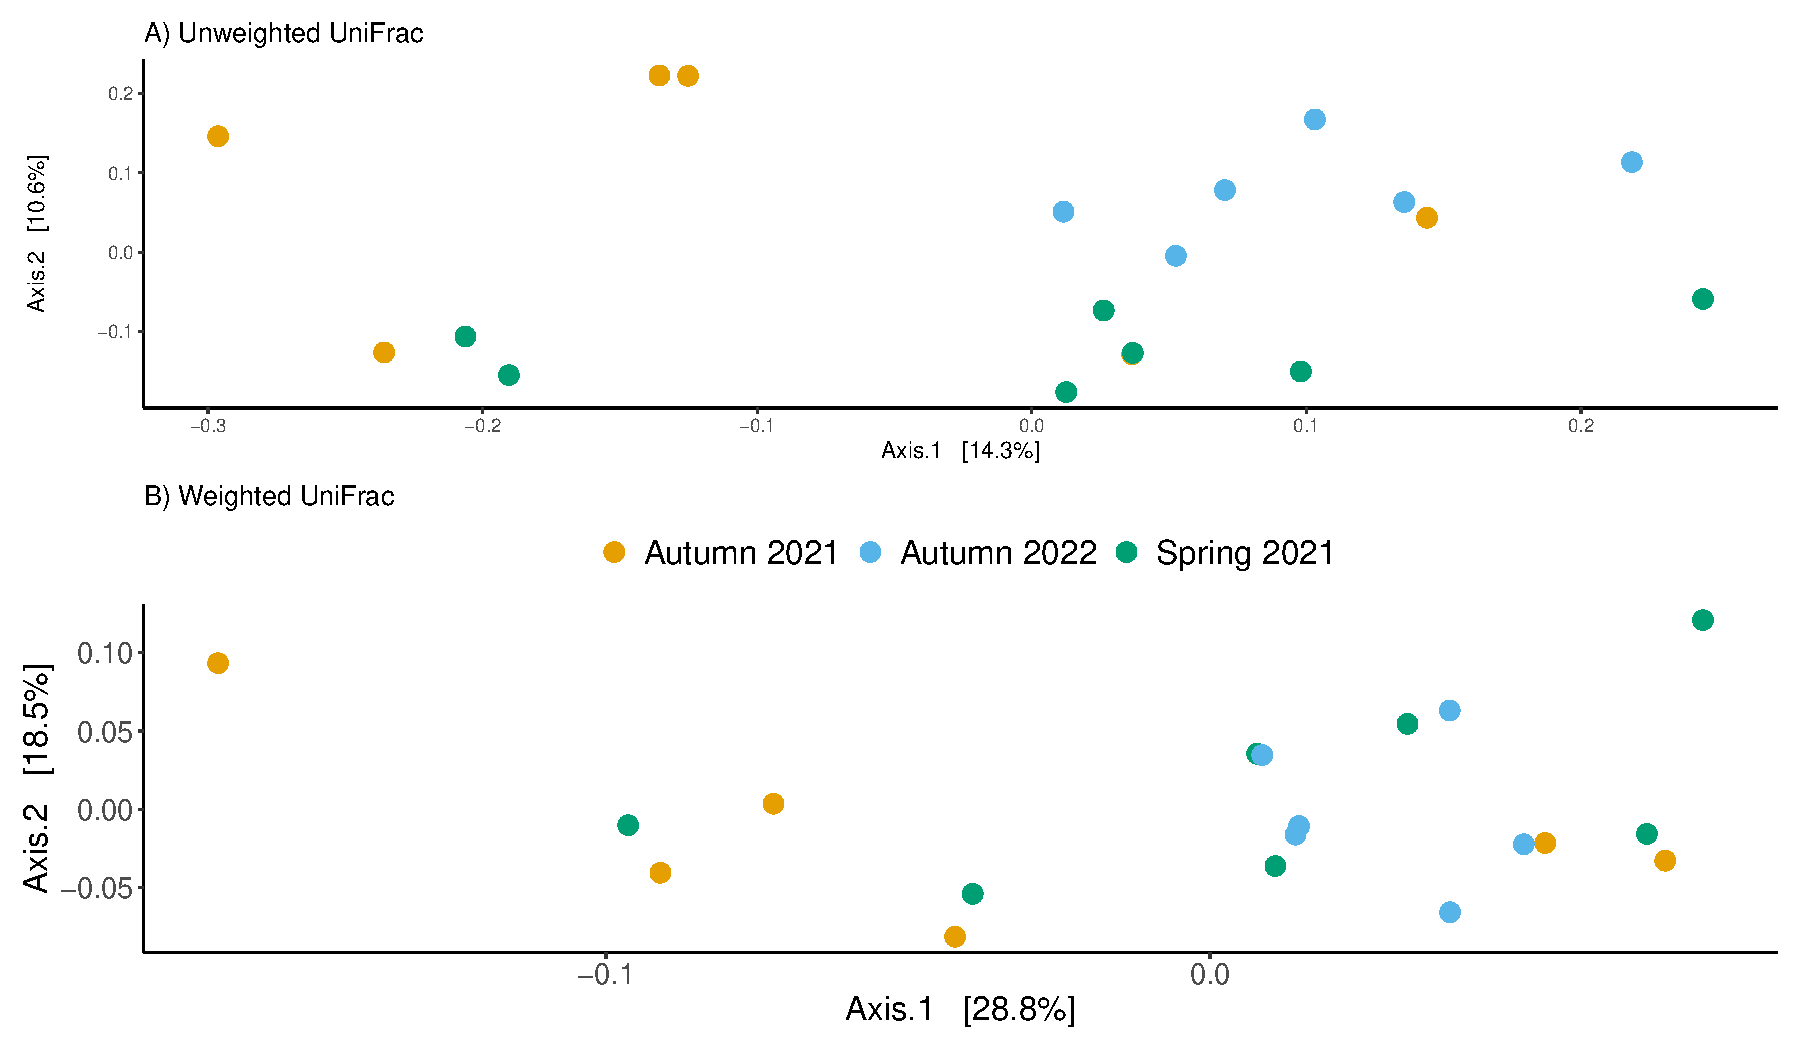
\includegraphics{code_files/figure-pdf/unnamed-chunk-7-2.pdf}

\begin{Shaded}
\begin{Highlighting}[]
\FunctionTok{ggsave}\NormalTok{(}\StringTok{"../figures/beta\_div\_ital\_1\_2.png"}\NormalTok{, }\AttributeTok{plot =}\NormalTok{ ital\_combined, }\AttributeTok{height =} \DecValTok{10}\NormalTok{, }\AttributeTok{width =} \DecValTok{10}\NormalTok{)}
\end{Highlighting}
\end{Shaded}

We again see variation associated with season across axis 1 for
unweighted unifrac for Bimbowrie, but not so much for Italowie. (Didn't
run stats for these, but can if we want to include them in the final
paper???)

\subsubsection{Taxa bar plots (all
samples)}\label{taxa-bar-plots-all-samples}

\begin{Shaded}
\begin{Highlighting}[]
\FunctionTok{library}\NormalTok{(microshades)}
\FunctionTok{library}\NormalTok{(ggh4x)}

\NormalTok{py\_mdf }\OtherTok{\textless{}{-}}\NormalTok{ ps\_adults }\SpecialCharTok{\%\textgreater{}\%}
  \FunctionTok{tax\_glom}\NormalTok{(}\StringTok{"Genus"}\NormalTok{) }\SpecialCharTok{\%\textgreater{}\%}
\NormalTok{  phyloseq}\SpecialCharTok{::}\FunctionTok{transform\_sample\_counts}\NormalTok{(}\ControlFlowTok{function}\NormalTok{(x) \{ x}\SpecialCharTok{/}\FunctionTok{sum}\NormalTok{(x) \}) }\SpecialCharTok{\%\textgreater{}\%}
  \FunctionTok{psmelt}\NormalTok{() }\SpecialCharTok{\%\textgreater{}\%}
  \FunctionTok{filter}\NormalTok{(Abundance }\SpecialCharTok{\textgreater{}} \DecValTok{0}\NormalTok{)}

\CommentTok{\#get the top 6 most abundant phyla}
\NormalTok{counts }\OtherTok{\textless{}{-}}\NormalTok{ ps\_adults }\SpecialCharTok{\%\textgreater{}\%}
  \FunctionTok{tax\_glom}\NormalTok{(}\StringTok{"Genus"}\NormalTok{) }\SpecialCharTok{\%\textgreater{}\%}
  \FunctionTok{psmelt}\NormalTok{()}
\NormalTok{mean }\OtherTok{\textless{}{-}}\NormalTok{ counts }\SpecialCharTok{\%\textgreater{}\%}
  \FunctionTok{group\_by}\NormalTok{(Phylum) }\SpecialCharTok{\%\textgreater{}\%}
  \FunctionTok{summarise}\NormalTok{(}\AttributeTok{relab =} \FunctionTok{sum}\NormalTok{(Abundance))}

\NormalTok{mean}
\end{Highlighting}
\end{Shaded}

\begin{verbatim}
# A tibble: 13 x 2
   Phylum             relab
   <chr>              <dbl>
 1 Actinobacteriota     173
 2 Bacteroidota      100866
 3 Campilobacterota    1050
 4 Cyanobacteria       3674
 5 Desulfobacterota    1972
 6 Elusimicrobiota      115
 7 Firmicutes        143738
 8 Halobacterota        365
 9 Planctomycetota      279
10 Proteobacteria      2326
11 Spirochaetota         52
12 Thermoplasmatota      30
13 Verrucomicrobiota  18376
\end{verbatim}

\begin{Shaded}
\begin{Highlighting}[]
\NormalTok{ms\_py }\OtherTok{\textless{}{-}} \FunctionTok{create\_color\_dfs}\NormalTok{(py\_mdf, }
                          \AttributeTok{selected\_groups =} \FunctionTok{c}\NormalTok{(}\StringTok{\textquotesingle{}Firmicutes\textquotesingle{}}\NormalTok{,}
                                              \StringTok{\textquotesingle{}Bacteroidota\textquotesingle{}}\NormalTok{,}
                                              \StringTok{\textquotesingle{}Verrucomicrobiota\textquotesingle{}}\NormalTok{,}
                                              \StringTok{\textquotesingle{}Cyanobacteria\textquotesingle{}}\NormalTok{,}
                                              \StringTok{\textquotesingle{}Proteobacteria\textquotesingle{}}\NormalTok{),}
                          \AttributeTok{group\_level =} \StringTok{"Phylum"}\NormalTok{, }
                          \AttributeTok{subgroup\_level =} \StringTok{"Genus"}\NormalTok{, }
                          \AttributeTok{cvd =} \ConstantTok{TRUE}\NormalTok{)}


\FunctionTok{plot\_microshades}\NormalTok{(ms\_py}\SpecialCharTok{$}\NormalTok{mdf, }
                 \AttributeTok{cdf =}\NormalTok{ ms\_py}\SpecialCharTok{$}\NormalTok{cdf, }
                 \AttributeTok{group\_label =} \StringTok{"Phylum Genus"}\NormalTok{) }\SpecialCharTok{+}
  \FunctionTok{facet\_nested}\NormalTok{(}\SpecialCharTok{\textasciitilde{}}\NormalTok{Location }\SpecialCharTok{+}\NormalTok{ Sampling\_trip,}
               \AttributeTok{space =} \StringTok{"free"}\NormalTok{,}
               \AttributeTok{scale =} \StringTok{"free"}\NormalTok{) }\SpecialCharTok{+}
  \FunctionTok{scale\_y\_continuous}\NormalTok{(}\AttributeTok{labels =}\NormalTok{ scales}\SpecialCharTok{::}\NormalTok{percent, }
                     \AttributeTok{expand =} \FunctionTok{expansion}\NormalTok{(}\DecValTok{0}\NormalTok{)) }\SpecialCharTok{+}
  \FunctionTok{theme\_classic}\NormalTok{() }\SpecialCharTok{+}
  \FunctionTok{theme}\NormalTok{(}
    \AttributeTok{legend.position =} \StringTok{"bottom"}\NormalTok{,}
    \AttributeTok{legend.title =} \FunctionTok{element\_blank}\NormalTok{(),}
    \AttributeTok{axis.text.x =} \FunctionTok{element\_blank}\NormalTok{(),}
    \AttributeTok{strip.text =} \FunctionTok{element\_text}\NormalTok{(}\AttributeTok{size =} \DecValTok{16}\NormalTok{, }\AttributeTok{face =} \StringTok{"bold"}\NormalTok{)}
\NormalTok{  ) }\SpecialCharTok{+}
  \FunctionTok{xlab}\NormalTok{(}\StringTok{""}\NormalTok{) }\SpecialCharTok{+}
  \FunctionTok{ylab}\NormalTok{(}\StringTok{"Relative abundance (\%)"}\NormalTok{)}
\end{Highlighting}
\end{Shaded}

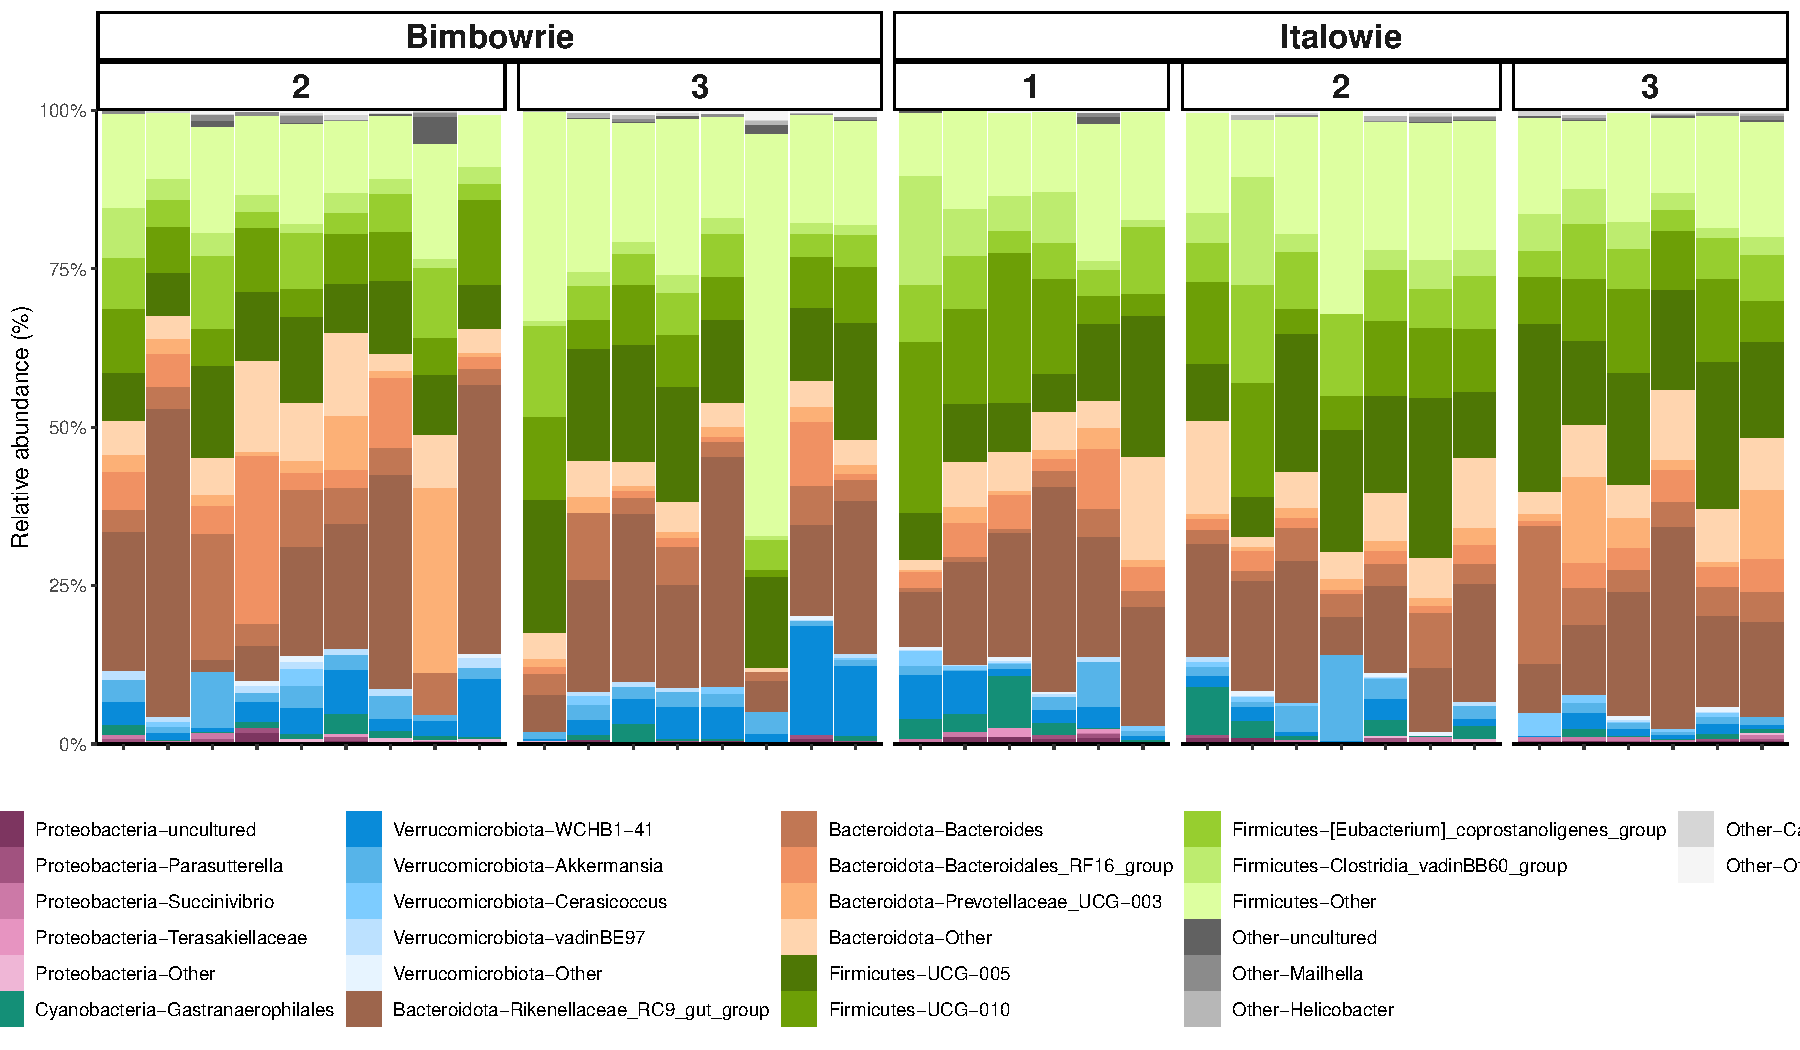
\includegraphics{code_files/figure-pdf/unnamed-chunk-8-1.pdf}

Nothing really jumps out here.

\subsubsection{Taxa bar subset of
samples}\label{taxa-bar-subset-of-samples}

\begin{Shaded}
\begin{Highlighting}[]
\FunctionTok{library}\NormalTok{(microshades)}
\FunctionTok{library}\NormalTok{(ggh4x)}

\NormalTok{sampleset1 }\OtherTok{\textless{}{-}} \FunctionTok{c}\NormalTok{(}\StringTok{"Patrick"}\NormalTok{, }\StringTok{"Peter"}\NormalTok{, }\StringTok{"Polly"}\NormalTok{, }\StringTok{"Pumpkin"}\NormalTok{,}
                \StringTok{"Petra"}\NormalTok{, }\StringTok{"Pickle"}\NormalTok{, }\StringTok{"Pedro"}\NormalTok{)}

\NormalTok{ps\_subset1 }\OtherTok{\textless{}{-}} \FunctionTok{subset\_samples}\NormalTok{(ps\_adults, }
\NormalTok{                             Dam\_name }\SpecialCharTok{\%in\%}\NormalTok{ sampleset1)}
\NormalTok{ps\_subset1 }\OtherTok{\textless{}{-}} \FunctionTok{subset\_samples}\NormalTok{(ps\_subset1, }
\NormalTok{                             sample\_name }\SpecialCharTok{!=} \StringTok{"35{-}21FBIMB3rd"}\NormalTok{)}
\NormalTok{ps\_subset1 }\OtherTok{\textless{}{-}} \FunctionTok{subset\_samples}\NormalTok{(ps\_subset1, }
\NormalTok{                             sample\_name }\SpecialCharTok{!=} \StringTok{"42{-}21FBIMB2nd"}\NormalTok{)}



\NormalTok{py\_mdf }\OtherTok{\textless{}{-}}\NormalTok{ ps\_subset1 }\SpecialCharTok{\%\textgreater{}\%}
  \FunctionTok{tax\_glom}\NormalTok{(}\StringTok{"Genus"}\NormalTok{) }\SpecialCharTok{\%\textgreater{}\%}
\NormalTok{  phyloseq}\SpecialCharTok{::}\FunctionTok{transform\_sample\_counts}\NormalTok{(}\ControlFlowTok{function}\NormalTok{(x) \{ x}\SpecialCharTok{/}\FunctionTok{sum}\NormalTok{(x) \}) }\SpecialCharTok{\%\textgreater{}\%}
  \FunctionTok{psmelt}\NormalTok{() }\SpecialCharTok{\%\textgreater{}\%}
  \FunctionTok{filter}\NormalTok{(Abundance }\SpecialCharTok{\textgreater{}} \DecValTok{0}\NormalTok{)}

\CommentTok{\#get the top 6 most abundant phyla}
\NormalTok{counts }\OtherTok{\textless{}{-}}\NormalTok{ ps\_subset1 }\SpecialCharTok{\%\textgreater{}\%}
  \FunctionTok{tax\_glom}\NormalTok{(}\StringTok{"Genus"}\NormalTok{) }\SpecialCharTok{\%\textgreater{}\%}
  \FunctionTok{psmelt}\NormalTok{()}
\NormalTok{mean }\OtherTok{\textless{}{-}}\NormalTok{ counts }\SpecialCharTok{\%\textgreater{}\%}
  \FunctionTok{group\_by}\NormalTok{(Phylum) }\SpecialCharTok{\%\textgreater{}\%}
  \FunctionTok{summarise}\NormalTok{(}\AttributeTok{relab =} \FunctionTok{sum}\NormalTok{(Abundance))}

\NormalTok{mean}
\end{Highlighting}
\end{Shaded}

\begin{verbatim}
# A tibble: 13 x 2
   Phylum            relab
   <chr>             <dbl>
 1 Actinobacteriota    118
 2 Bacteroidota      24609
 3 Campilobacterota    197
 4 Cyanobacteria       354
 5 Desulfobacterota    475
 6 Elusimicrobiota       0
 7 Firmicutes        30343
 8 Halobacterota        70
 9 Planctomycetota     124
10 Proteobacteria      306
11 Spirochaetota         0
12 Thermoplasmatota      0
13 Verrucomicrobiota  4545
\end{verbatim}

\begin{Shaded}
\begin{Highlighting}[]
\NormalTok{ms\_py }\OtherTok{\textless{}{-}} \FunctionTok{create\_color\_dfs}\NormalTok{(py\_mdf, }
                          \AttributeTok{selected\_groups =} \FunctionTok{c}\NormalTok{(}\StringTok{\textquotesingle{}Firmicutes\textquotesingle{}}\NormalTok{,}
                                              \StringTok{\textquotesingle{}Bacteroidota\textquotesingle{}}\NormalTok{,}
                                              \StringTok{\textquotesingle{}Verrucomicrobiota\textquotesingle{}}\NormalTok{,}
                                              \StringTok{\textquotesingle{}Cyanobacteria\textquotesingle{}}\NormalTok{,}
                                              \StringTok{\textquotesingle{}Proteobacteria\textquotesingle{}}\NormalTok{),}
                          \AttributeTok{group\_level =} \StringTok{"Phylum"}\NormalTok{, }
                          \AttributeTok{subgroup\_level =} \StringTok{"Genus"}\NormalTok{, }
                          \AttributeTok{cvd =} \ConstantTok{TRUE}\NormalTok{)}

\CommentTok{\#reorder factors}
\NormalTok{ms\_py}\SpecialCharTok{$}\NormalTok{mdf}\SpecialCharTok{$}\NormalTok{season }\OtherTok{\textless{}{-}} \FunctionTok{factor}\NormalTok{(ms\_py}\SpecialCharTok{$}\NormalTok{mdf}\SpecialCharTok{$}\NormalTok{season,}
                           \AttributeTok{levels =} \FunctionTok{c}\NormalTok{(}\StringTok{"Spring 2021"}\NormalTok{, }\StringTok{"Autumn 2022"}\NormalTok{))}

\FunctionTok{plot\_microshades}\NormalTok{(ms\_py}\SpecialCharTok{$}\NormalTok{mdf, }
                 \AttributeTok{cdf =}\NormalTok{ ms\_py}\SpecialCharTok{$}\NormalTok{cdf, }
                 \AttributeTok{group\_label =} \StringTok{"Phylum Genus"}\NormalTok{,}
                 \AttributeTok{x =} \StringTok{"Dam\_name"}\NormalTok{) }\SpecialCharTok{+}
  \FunctionTok{facet\_nested}\NormalTok{(}\SpecialCharTok{\textasciitilde{}}\NormalTok{season,}
               \AttributeTok{space =} \StringTok{"free"}\NormalTok{,}
               \AttributeTok{scale =} \StringTok{"free"}\NormalTok{, ) }\SpecialCharTok{+}
  \FunctionTok{scale\_y\_continuous}\NormalTok{(}\AttributeTok{labels =}\NormalTok{ scales}\SpecialCharTok{::}\NormalTok{percent, }
                     \AttributeTok{expand =} \FunctionTok{expansion}\NormalTok{(}\DecValTok{0}\NormalTok{)) }\SpecialCharTok{+}
  \FunctionTok{theme\_classic}\NormalTok{() }\SpecialCharTok{+}
  \FunctionTok{theme}\NormalTok{(}
    \AttributeTok{legend.position =} \StringTok{"bottom"}\NormalTok{,}
    \AttributeTok{legend.title =} \FunctionTok{element\_blank}\NormalTok{(),}
    \AttributeTok{legend.text =} \FunctionTok{element\_text}\NormalTok{(}\AttributeTok{size =} \DecValTok{12}\NormalTok{),}
    \AttributeTok{axis.text.x =} \FunctionTok{element\_text}\NormalTok{(}\AttributeTok{angle =} \DecValTok{90}\NormalTok{, }\AttributeTok{size =} \DecValTok{14}\NormalTok{, }\AttributeTok{face =} \StringTok{"bold"}\NormalTok{),}
    \AttributeTok{strip.text =} \FunctionTok{element\_text}\NormalTok{(}\AttributeTok{size =} \DecValTok{16}\NormalTok{, }\AttributeTok{face =} \StringTok{"bold"}\NormalTok{)}
\NormalTok{  ) }\SpecialCharTok{+}
  \FunctionTok{xlab}\NormalTok{(}\StringTok{""}\NormalTok{) }\SpecialCharTok{+}
  \FunctionTok{ylab}\NormalTok{(}\StringTok{"Relative abundance (\%)"}\NormalTok{)}
\end{Highlighting}
\end{Shaded}

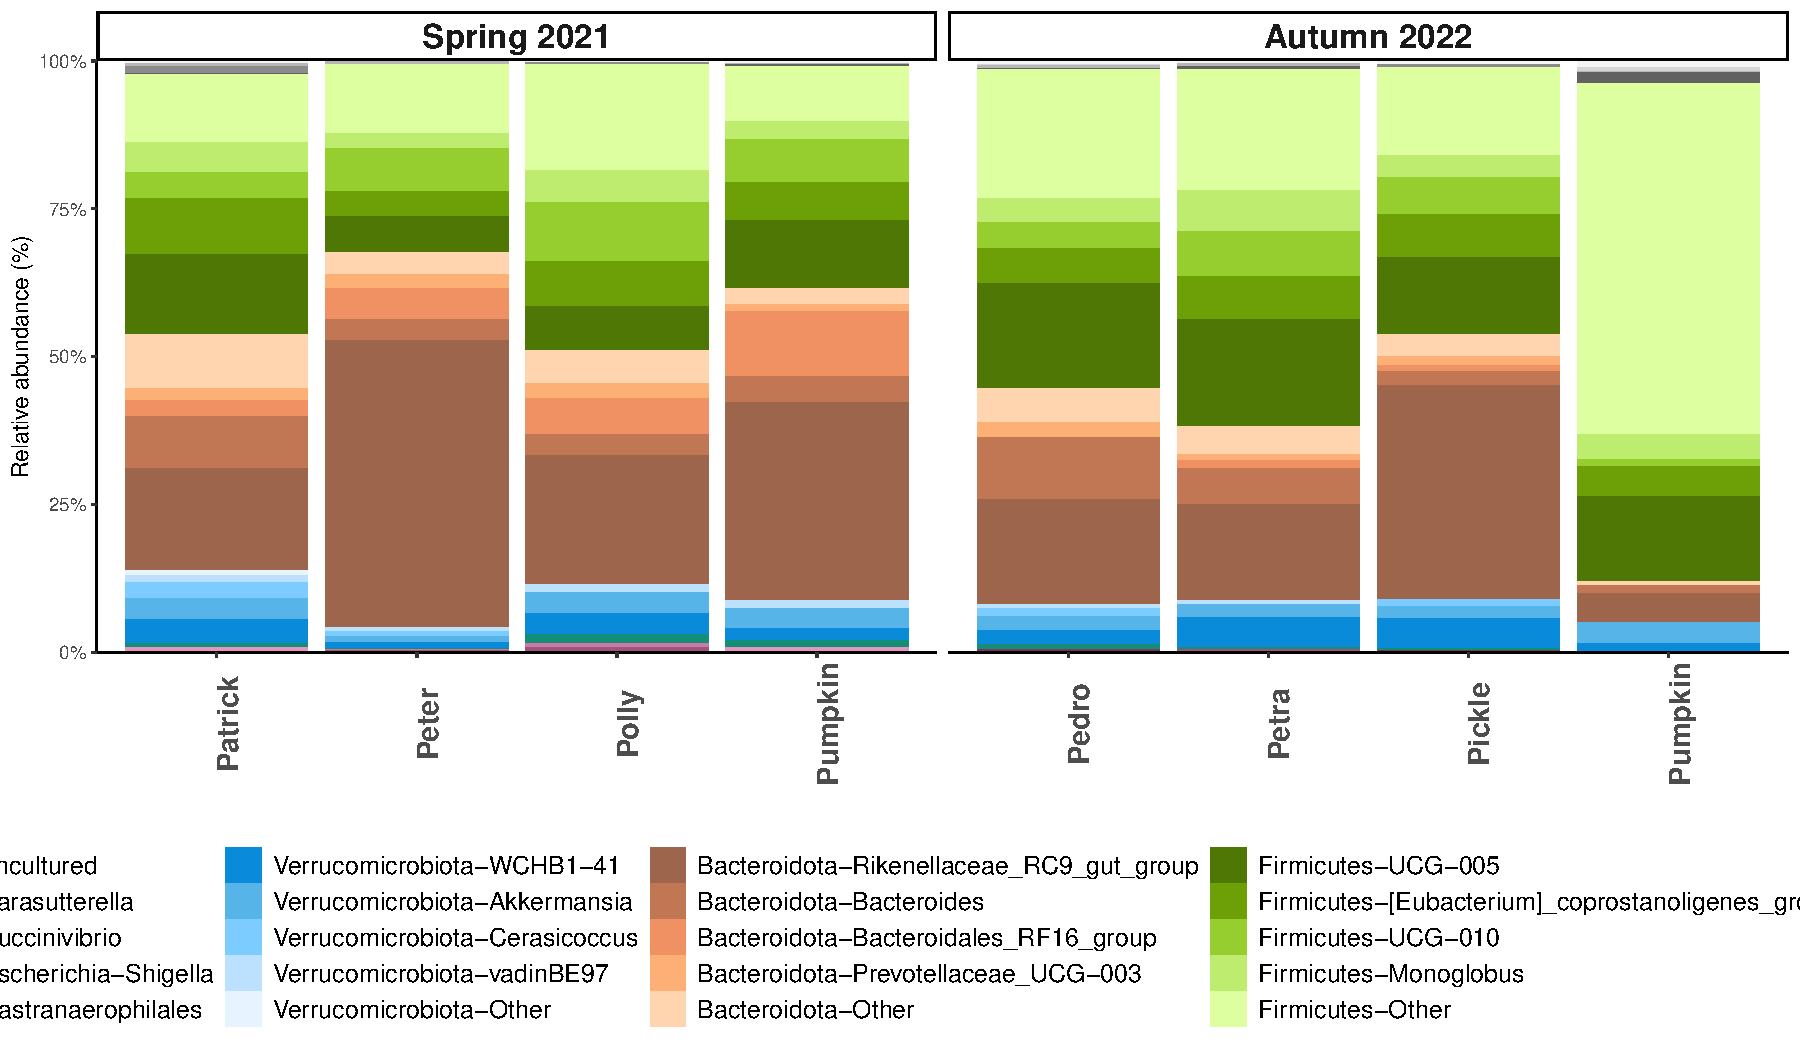
\includegraphics{code_files/figure-pdf/unnamed-chunk-9-1.pdf}

\subsubsection{Taxa bar subset of samples
(2)}\label{taxa-bar-subset-of-samples-2}

\begin{Shaded}
\begin{Highlighting}[]
\FunctionTok{library}\NormalTok{(microshades)}
\FunctionTok{library}\NormalTok{(ggh4x)}

\NormalTok{sampleset2 }\OtherTok{\textless{}{-}} \FunctionTok{c}\NormalTok{(}\StringTok{"Judd"}\NormalTok{, }\StringTok{"Zara"}\NormalTok{, }\StringTok{"Eileen"}\NormalTok{, }\StringTok{"Elton"}\NormalTok{,}
                \StringTok{"Max"}\NormalTok{, }\StringTok{"Lola"}\NormalTok{, }\StringTok{"Meatloaf"}\NormalTok{, }\StringTok{"Rosie"}\NormalTok{,}
                \StringTok{"Tags"}\NormalTok{, }\StringTok{"Valerie"}\NormalTok{, }\StringTok{"Adele"}\NormalTok{, }\StringTok{"Brandy"}\NormalTok{,}
                \StringTok{"Cecilia"}\NormalTok{)}

\NormalTok{ps\_subset2 }\OtherTok{\textless{}{-}} \FunctionTok{subset\_samples}\NormalTok{(ps\_adults, }
\NormalTok{                             Dam\_name }\SpecialCharTok{\%in\%}\NormalTok{ sampleset2)}
\NormalTok{ps\_subset2 }\OtherTok{\textless{}{-}} \FunctionTok{subset\_samples}\NormalTok{(ps\_subset2, }
\NormalTok{                             sample\_name }\SpecialCharTok{!=} \StringTok{"2{-}21FITA1st"}\NormalTok{)}




\NormalTok{py\_mdf }\OtherTok{\textless{}{-}}\NormalTok{ ps\_subset2 }\SpecialCharTok{\%\textgreater{}\%}
  \FunctionTok{tax\_glom}\NormalTok{(}\StringTok{"Genus"}\NormalTok{) }\SpecialCharTok{\%\textgreater{}\%}
\NormalTok{  phyloseq}\SpecialCharTok{::}\FunctionTok{transform\_sample\_counts}\NormalTok{(}\ControlFlowTok{function}\NormalTok{(x) \{ x}\SpecialCharTok{/}\FunctionTok{sum}\NormalTok{(x) \}) }\SpecialCharTok{\%\textgreater{}\%}
  \FunctionTok{psmelt}\NormalTok{() }\SpecialCharTok{\%\textgreater{}\%}
  \FunctionTok{filter}\NormalTok{(Abundance }\SpecialCharTok{\textgreater{}} \DecValTok{0}\NormalTok{)}

\CommentTok{\#get the top 6 most abundant phyla}
\NormalTok{counts }\OtherTok{\textless{}{-}}\NormalTok{ ps\_subset2 }\SpecialCharTok{\%\textgreater{}\%}
  \FunctionTok{tax\_glom}\NormalTok{(}\StringTok{"Genus"}\NormalTok{) }\SpecialCharTok{\%\textgreater{}\%}
  \FunctionTok{psmelt}\NormalTok{()}
\NormalTok{mean }\OtherTok{\textless{}{-}}\NormalTok{ counts }\SpecialCharTok{\%\textgreater{}\%}
  \FunctionTok{group\_by}\NormalTok{(Phylum) }\SpecialCharTok{\%\textgreater{}\%}
  \FunctionTok{summarise}\NormalTok{(}\AttributeTok{relab =} \FunctionTok{sum}\NormalTok{(Abundance))}

\NormalTok{ms\_py }\OtherTok{\textless{}{-}} \FunctionTok{create\_color\_dfs}\NormalTok{(py\_mdf, }
                          \AttributeTok{selected\_groups =} \FunctionTok{c}\NormalTok{(}\StringTok{\textquotesingle{}Firmicutes\textquotesingle{}}\NormalTok{,}
                                              \StringTok{\textquotesingle{}Bacteroidota\textquotesingle{}}\NormalTok{,}
                                              \StringTok{\textquotesingle{}Verrucomicrobiota\textquotesingle{}}\NormalTok{,}
                                              \StringTok{\textquotesingle{}Cyanobacteria\textquotesingle{}}\NormalTok{,}
                                              \StringTok{\textquotesingle{}Proteobacteria\textquotesingle{}}\NormalTok{),}
                          \AttributeTok{group\_level =} \StringTok{"Phylum"}\NormalTok{, }
                          \AttributeTok{subgroup\_level =} \StringTok{"Genus"}\NormalTok{, }
                          \AttributeTok{cvd =} \ConstantTok{TRUE}\NormalTok{)}

\CommentTok{\#reorder factors}
\NormalTok{ms\_py}\SpecialCharTok{$}\NormalTok{mdf}\SpecialCharTok{$}\NormalTok{season }\OtherTok{\textless{}{-}} \FunctionTok{factor}\NormalTok{(ms\_py}\SpecialCharTok{$}\NormalTok{mdf}\SpecialCharTok{$}\NormalTok{season,}
                           \AttributeTok{levels =} \FunctionTok{c}\NormalTok{(}\StringTok{"Autumn 2021"}\NormalTok{, }\StringTok{"Spring 2021"}\NormalTok{, }\StringTok{"Autumn 2022"}\NormalTok{))}

\FunctionTok{plot\_microshades}\NormalTok{(ms\_py}\SpecialCharTok{$}\NormalTok{mdf, }
                 \AttributeTok{cdf =}\NormalTok{ ms\_py}\SpecialCharTok{$}\NormalTok{cdf, }
                 \AttributeTok{group\_label =} \StringTok{"Phylum Genus"}\NormalTok{,}
                 \AttributeTok{x =} \StringTok{"Dam\_name"}\NormalTok{) }\SpecialCharTok{+}
  \FunctionTok{facet\_nested}\NormalTok{(}\SpecialCharTok{\textasciitilde{}}\NormalTok{season,}
               \AttributeTok{space =} \StringTok{"free"}\NormalTok{,}
               \AttributeTok{scale =} \StringTok{"free"}\NormalTok{, ) }\SpecialCharTok{+}
  \FunctionTok{scale\_y\_continuous}\NormalTok{(}\AttributeTok{labels =}\NormalTok{ scales}\SpecialCharTok{::}\NormalTok{percent, }
                     \AttributeTok{expand =} \FunctionTok{expansion}\NormalTok{(}\DecValTok{0}\NormalTok{)) }\SpecialCharTok{+}
  \FunctionTok{theme\_classic}\NormalTok{() }\SpecialCharTok{+}
  \FunctionTok{theme}\NormalTok{(}
    \AttributeTok{legend.position =} \StringTok{"bottom"}\NormalTok{,}
    \AttributeTok{legend.title =} \FunctionTok{element\_blank}\NormalTok{(),}
    \AttributeTok{legend.text =} \FunctionTok{element\_text}\NormalTok{(}\AttributeTok{size =} \DecValTok{12}\NormalTok{),}
    \AttributeTok{axis.text.x =} \FunctionTok{element\_text}\NormalTok{(}\AttributeTok{angle =} \DecValTok{90}\NormalTok{, }\AttributeTok{size =} \DecValTok{14}\NormalTok{, }\AttributeTok{face =} \StringTok{"bold"}\NormalTok{),}
    \AttributeTok{strip.text =} \FunctionTok{element\_text}\NormalTok{(}\AttributeTok{size =} \DecValTok{16}\NormalTok{, }\AttributeTok{face =} \StringTok{"bold"}\NormalTok{)}
\NormalTok{  ) }\SpecialCharTok{+}
  \FunctionTok{xlab}\NormalTok{(}\StringTok{""}\NormalTok{) }\SpecialCharTok{+}
  \FunctionTok{ylab}\NormalTok{(}\StringTok{"Relative abundance (\%)"}\NormalTok{)}
\end{Highlighting}
\end{Shaded}

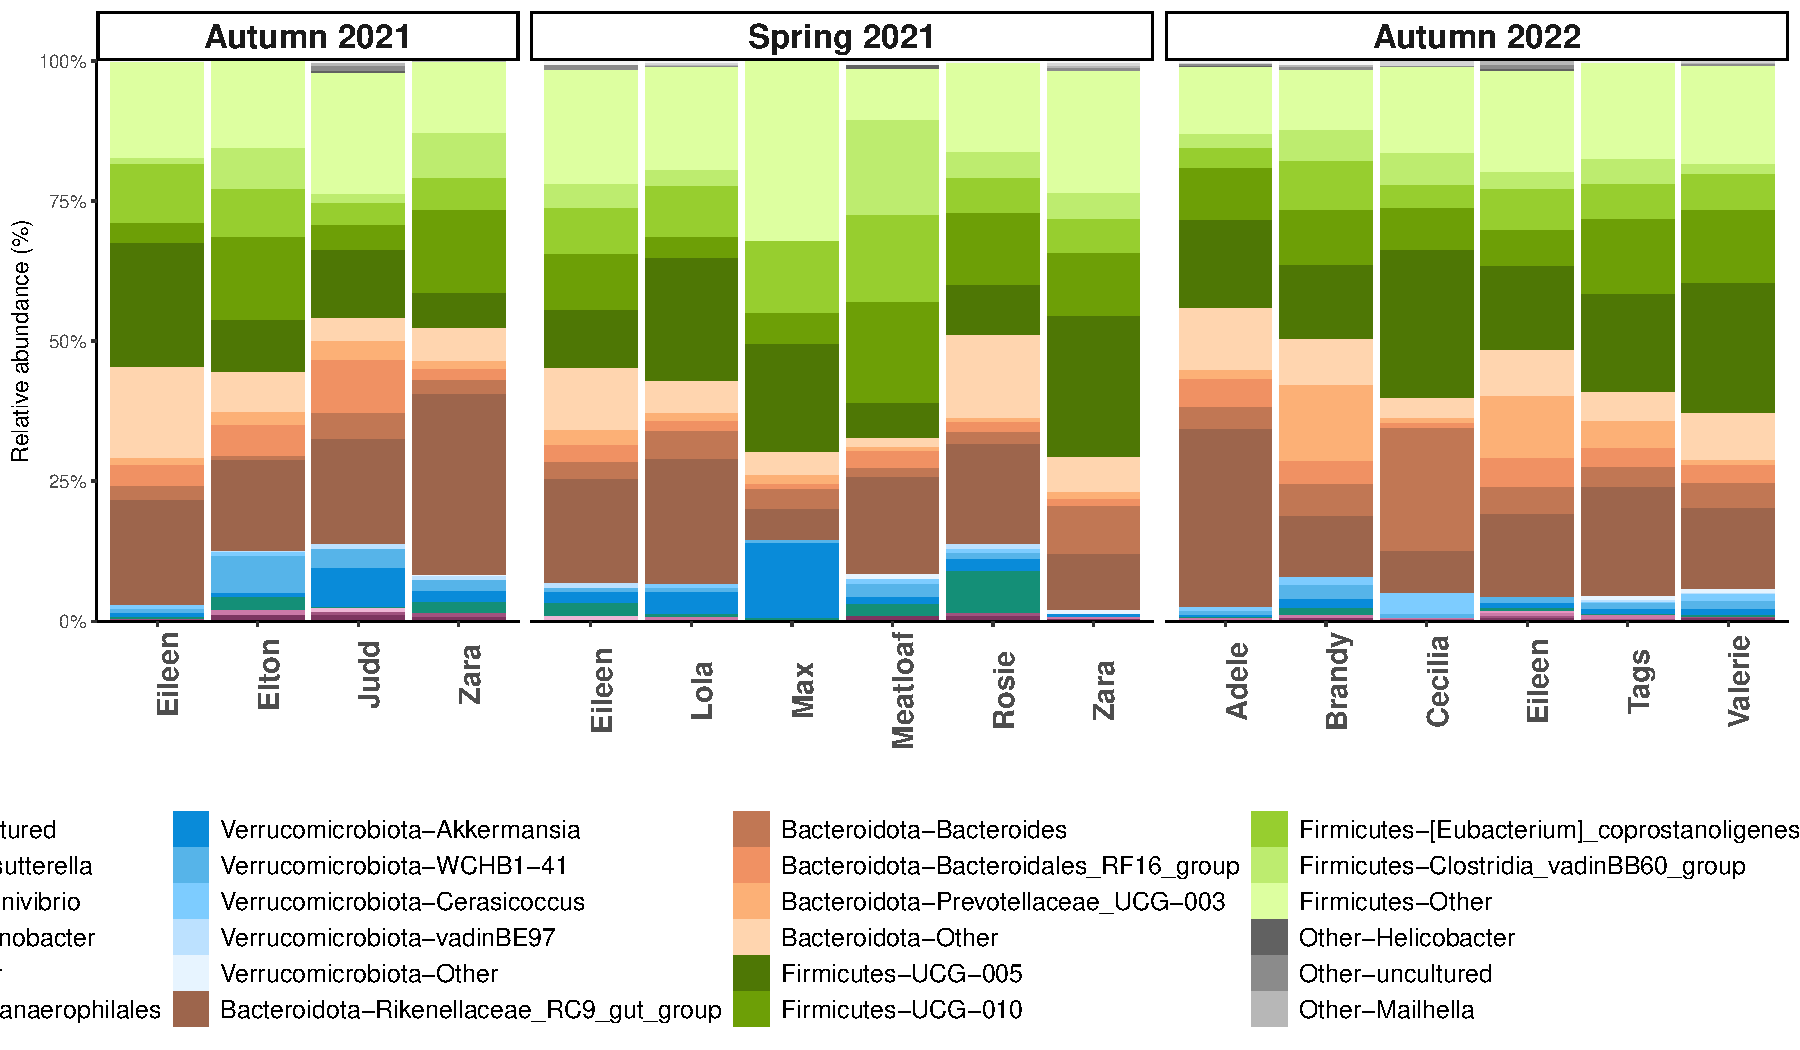
\includegraphics{code_files/figure-pdf/unnamed-chunk-10-1.pdf}

\subsubsection{Differential abundance with
ANCOMBC-2}\label{differential-abundance-with-ancombc-2}

\begin{Shaded}
\begin{Highlighting}[]
\CommentTok{\# library(ANCOMBC)}
\CommentTok{\# }
\CommentTok{\# ps\_adults\_glom \textless{}{-} ps\_adults \%\textgreater{}\%}
\CommentTok{\#   tax\_glom("Genus")}
\CommentTok{\# }
\CommentTok{\# \#Run ancombc2: Location \& season as fixed effects, individual as random effect}
\CommentTok{\# \# ancombc2\_location \textless{}{-} ancombc2(data = ps\_adults,}
\CommentTok{\# \#                               assay\_name = "counts",}
\CommentTok{\# \#                               tax\_level = "Genus",}
\CommentTok{\# \#                               fix\_formula = "Location + season",}
\CommentTok{\# \#                               rand\_formula = "(1 | Dam\_name)",}
\CommentTok{\# \#                               lib\_cut = 6000,}
\CommentTok{\# \#                               n\_cl = 4)}
\CommentTok{\# }
\CommentTok{\# }
\CommentTok{\# \#save output}
\CommentTok{\# saveRDS(ancombc2\_location, "../data/ancombc\_location\_season\_individual.rds")}
\CommentTok{\# saveRDS(ancombc2\_location\_asv, "../data/ancombc2\_location\_season\_asv.rds")}
\CommentTok{\# }
\CommentTok{\# \#Split table by location, then run testing for season}
\CommentTok{\# }
\CommentTok{\# ps\_bimba \textless{}{-} subset\_samples(ps\_adults, Location == "Bimbowrie")}
\CommentTok{\# ps\_italo \textless{}{-} subset\_samples(ps\_adults, Location == "Italowie")}
\CommentTok{\# }
\CommentTok{\# ps\_bimba\_glom \textless{}{-} ps\_bimba \%\textgreater{}\%}
\CommentTok{\#   tax\_glom("Genus")}
\CommentTok{\# ps\_italo\_glom \textless{}{-} ps\_italo \%\textgreater{}\%}
\CommentTok{\#   tax\_glom("Genus")}
\CommentTok{\# }
\CommentTok{\# \# ancombc2\_bimba\_season\_asv \textless{}{-} ancombc2(data = ps\_bimba,}
\CommentTok{\# \#                               assay\_name = "counts",}
\CommentTok{\# \# \#                              tax\_level = "Genus",}
\CommentTok{\# \#                               fix\_formula = "season",}
\CommentTok{\# \#                               rand\_formula = "(1 | Dam\_name)",}
\CommentTok{\# \#                               lme\_control = lme4::lmerControl(),}
\CommentTok{\# \#                               lib\_cut = 6000,}
\CommentTok{\# \#                               n\_cl = 4)}
\CommentTok{\# \# }
\CommentTok{\# \# }
\CommentTok{\# \# saveRDS(ancombc2\_bimba\_season\_glom, "../data/ancombc2\_bimba\_season\_glom.rds")}
\CommentTok{\# \# }
\CommentTok{\# \# }
\CommentTok{\# \# ancombc2\_italo\_season \textless{}{-} ancombc2(data = ps\_italo,}
\CommentTok{\# \#                               assay\_name = "counts",}
\CommentTok{\# \# \#                              tax\_level = "Genus",}
\CommentTok{\# \#                               fix\_formula = "season",}
\CommentTok{\# \# \#                              rand\_formula = "(1 | Dam\_name)",}
\CommentTok{\# \#                               lme\_control = lme4::lmerControl(),}
\CommentTok{\# \#                               lib\_cut = 6000,}
\CommentTok{\# \#                               n\_cl = 4)}
\CommentTok{\# \# }
\CommentTok{\# \# }
\CommentTok{\# \# saveRDS(ancombc2\_italo\_season, "../data/ancombc2\_italo\_season\_glom.rds")}
\CommentTok{\# }
\CommentTok{\# }
\CommentTok{\# }
\CommentTok{\# bimb\_season \textless{}{-} readRDS("../data/ancombc2\_bimba\_season.rds")}
\CommentTok{\# }
\CommentTok{\# ital\_season \textless{}{-} readRDS("../data/ancombc2\_italo\_season.rds")}
\CommentTok{\# }
\CommentTok{\# ancom\_all \textless{}{-} ancombc2\_location$res}
\CommentTok{\# ancom\_all\_glom \textless{}{-} ancombc2\_location\_glom$res}
\CommentTok{\# ancom\_bimb \textless{}{-} ancombc2\_bimba\_season$res}
\CommentTok{\# ancom\_bimb\_glom \textless{}{-} ancombc2\_bimba\_season\_glom$res}
\CommentTok{\# ancom\_ital\_glom \textless{}{-} ancombc2\_italo\_season$res}
\CommentTok{\# ancom\_bimb\_asv \textless{}{-} ancombc2\_bimba\_season\_asv$res}
\CommentTok{\# ancom\_all\_asv \textless{}{-} ancombc2\_location\_asv$res}
\end{Highlighting}
\end{Shaded}

\subsubsection{Venn diagrams of ASVs}\label{venn-diagrams-of-asvs}

\begin{Shaded}
\begin{Highlighting}[]
\FunctionTok{library}\NormalTok{(VennDiagram)}
\end{Highlighting}
\end{Shaded}

\begin{verbatim}
Loading required package: grid
\end{verbatim}

\begin{verbatim}
Loading required package: futile.logger
\end{verbatim}

\begin{Shaded}
\begin{Highlighting}[]
\FunctionTok{library}\NormalTok{(ggVennDiagram)}
\end{Highlighting}
\end{Shaded}

\begin{verbatim}

Attaching package: 'ggVennDiagram'
\end{verbatim}

\begin{verbatim}
The following object is masked from 'package:microbiome':

    overlap
\end{verbatim}

\begin{verbatim}
The following object is masked from 'package:tidyr':

    unite
\end{verbatim}

\begin{Shaded}
\begin{Highlighting}[]
\NormalTok{ps\_bimba }\OtherTok{\textless{}{-}} \FunctionTok{subset\_samples}\NormalTok{(ps\_adults, Location }\SpecialCharTok{==} \StringTok{"Bimbowrie"}\NormalTok{)}
\NormalTok{ps\_italo }\OtherTok{\textless{}{-}} \FunctionTok{subset\_samples}\NormalTok{(ps\_adults, Location }\SpecialCharTok{==} \StringTok{"Italowie"}\NormalTok{)}

\NormalTok{ps\_bimba\_table }\OtherTok{\textless{}{-}} \FunctionTok{otu\_table}\NormalTok{(ps\_bimba)}
\NormalTok{ps\_italo\_table }\OtherTok{\textless{}{-}} \FunctionTok{otu\_table}\NormalTok{(ps\_italo)}

\NormalTok{ps\_merged }\OtherTok{\textless{}{-}} \FunctionTok{merge\_phyloseq}\NormalTok{(ps\_bimba, ps\_italo)}
\NormalTok{ps\_merged\_filt }\OtherTok{\textless{}{-}} \FunctionTok{prune\_taxa}\NormalTok{(}\FunctionTok{taxa\_sums}\NormalTok{(ps\_merged) }\SpecialCharTok{\textgreater{}} \DecValTok{0}\NormalTok{, ps\_merged)}

\CommentTok{\#For each ASV (row), if abundance \textgreater{} 2, print ASV (rowname) to a vector}
\NormalTok{venn\_bimba }\OtherTok{\textless{}{-}} \FunctionTok{rownames}\NormalTok{(ps\_bimba\_table[ }\FunctionTok{apply}\NormalTok{(ps\_bimba\_table, }\AttributeTok{MARGIN =} \DecValTok{1}\NormalTok{,}
                                             \ControlFlowTok{function}\NormalTok{(x) }\FunctionTok{any}\NormalTok{(x }\SpecialCharTok{\textgreater{}} \DecValTok{2}\NormalTok{))])}

\NormalTok{venn\_italo }\OtherTok{\textless{}{-}} \FunctionTok{rownames}\NormalTok{(ps\_italo\_table[ }\FunctionTok{apply}\NormalTok{(ps\_italo\_table, }\AttributeTok{MARGIN =} \DecValTok{1}\NormalTok{,}
                                                  \ControlFlowTok{function}\NormalTok{(x) }\FunctionTok{any}\NormalTok{(x }\SpecialCharTok{\textgreater{}} \DecValTok{2}\NormalTok{))])}


\NormalTok{venn\_both }\OtherTok{\textless{}{-}} \FunctionTok{list}\NormalTok{(}\AttributeTok{Bimbowrie =}\NormalTok{ venn\_bimba, }
                  \AttributeTok{Italowie =}\NormalTok{ venn\_italo)}


\NormalTok{VennDiagram}\SpecialCharTok{::}\FunctionTok{venn.diagram}\NormalTok{(venn\_both, }
                          \AttributeTok{fill =} \FunctionTok{c}\NormalTok{(}\StringTok{"\#E69F00"}\NormalTok{, }\StringTok{"\#56B4E9"}\NormalTok{),}
                          \AttributeTok{disable.logging =} \ConstantTok{TRUE}\NormalTok{,}
                          \AttributeTok{alpha =} \FloatTok{0.5}\NormalTok{,}
                          \AttributeTok{filename =} \StringTok{"../figures/venn.png"}\NormalTok{,}
                          \AttributeTok{print.mode =} \FunctionTok{c}\NormalTok{(}\StringTok{"raw"}\NormalTok{,}\StringTok{"percent"}\NormalTok{))}
\end{Highlighting}
\end{Shaded}

\begin{verbatim}
INFO [2024-03-14 15:45:48] [[1]]
INFO [2024-03-14 15:45:48] venn_both
INFO [2024-03-14 15:45:48] 
INFO [2024-03-14 15:45:48] $fill
INFO [2024-03-14 15:45:48] c("#E69F00", "#56B4E9")
INFO [2024-03-14 15:45:48] 
INFO [2024-03-14 15:45:48] $disable.logging
INFO [2024-03-14 15:45:48] [1] TRUE
INFO [2024-03-14 15:45:48] 
INFO [2024-03-14 15:45:48] $alpha
INFO [2024-03-14 15:45:48] [1] 0.5
INFO [2024-03-14 15:45:48] 
INFO [2024-03-14 15:45:48] $filename
INFO [2024-03-14 15:45:48] [1] "../figures/venn.png"
INFO [2024-03-14 15:45:48] 
INFO [2024-03-14 15:45:48] $print.mode
INFO [2024-03-14 15:45:48] c("raw", "percent")
INFO [2024-03-14 15:45:48] 
\end{verbatim}

\begin{verbatim}
[1] 1
\end{verbatim}

\begin{Shaded}
\begin{Highlighting}[]
\DocumentationTok{\#\#Now, let\textquotesingle{}s pull out stats about the venn diagrams (i.e. what \% of ASVs and rel ab.)}
\CommentTok{\#Pull out ASVs belonging to specific regions venn diagram}
\NormalTok{venn }\OtherTok{\textless{}{-}} \FunctionTok{Venn}\NormalTok{(venn\_both)}
\NormalTok{venny }\OtherTok{\textless{}{-}} \FunctionTok{process\_data}\NormalTok{(venn, }\AttributeTok{shape\_id =} \StringTok{"201"}\NormalTok{)}
\NormalTok{venny\_df }\OtherTok{\textless{}{-}} \FunctionTok{as\_tibble}\NormalTok{(}\FunctionTok{venn\_region}\NormalTok{(venny))}

\NormalTok{bimba\_asvs }\OtherTok{\textless{}{-}}\NormalTok{ venny\_df }\SpecialCharTok{\%\textgreater{}\%}
  \FunctionTok{filter}\NormalTok{(id }\SpecialCharTok{==} \DecValTok{1}\NormalTok{) }\SpecialCharTok{\%\textgreater{}\%}
  \FunctionTok{pull}\NormalTok{(item) }\SpecialCharTok{\%\textgreater{}\%}
  \FunctionTok{pluck}\NormalTok{(}\DecValTok{1}\NormalTok{)}

\NormalTok{italo\_asvs }\OtherTok{\textless{}{-}}\NormalTok{ venny\_df }\SpecialCharTok{\%\textgreater{}\%}
  \FunctionTok{filter}\NormalTok{(id }\SpecialCharTok{==} \DecValTok{2}\NormalTok{) }\SpecialCharTok{\%\textgreater{}\%}
  \FunctionTok{pull}\NormalTok{(item) }\SpecialCharTok{\%\textgreater{}\%}
  \FunctionTok{pluck}\NormalTok{(}\DecValTok{1}\NormalTok{)}

\NormalTok{both\_asvs }\OtherTok{\textless{}{-}}\NormalTok{ venny\_df }\SpecialCharTok{\%\textgreater{}\%}
  \FunctionTok{filter}\NormalTok{(id }\SpecialCharTok{==} \StringTok{"1/2"}\NormalTok{) }\SpecialCharTok{\%\textgreater{}\%}
  \FunctionTok{pull}\NormalTok{(item) }\SpecialCharTok{\%\textgreater{}\%}
  \FunctionTok{pluck}\NormalTok{(}\DecValTok{1}\NormalTok{)}

\DocumentationTok{\#\#What\textquotesingle{}s the relative abundance of site{-}specific ASVs in each region?}
\CommentTok{\#Calculated as: number of reads for site{-}specific ASVs / number of reads for all ASVs at site}

\CommentTok{\#Bimba}
\NormalTok{percent\_bimba\_asv }\OtherTok{\textless{}{-}}\NormalTok{ scales}\SpecialCharTok{::}\FunctionTok{percent}\NormalTok{(}
  \FunctionTok{mean}\NormalTok{(}\FunctionTok{sample\_sums}\NormalTok{(}\FunctionTok{prune\_taxa}\NormalTok{(bimba\_asvs, ps\_bimba)))}\SpecialCharTok{/}
  \FunctionTok{mean}\NormalTok{(}\FunctionTok{sample\_sums}\NormalTok{(ps\_bimba))}
\NormalTok{)}
\CommentTok{\#Italo}
\NormalTok{percent\_italo\_asv }\OtherTok{\textless{}{-}}\NormalTok{ scales}\SpecialCharTok{::}\FunctionTok{percent}\NormalTok{(}
  \FunctionTok{mean}\NormalTok{(}\FunctionTok{sample\_sums}\NormalTok{(}\FunctionTok{prune\_taxa}\NormalTok{(italo\_asvs, ps\_italo)))}\SpecialCharTok{/}
  \FunctionTok{mean}\NormalTok{(}\FunctionTok{sample\_sums}\NormalTok{(ps\_italo))}
\NormalTok{)}
\CommentTok{\#Both}
\NormalTok{percent\_both\_asv }\OtherTok{\textless{}{-}}\NormalTok{ scales}\SpecialCharTok{::}\FunctionTok{percent}\NormalTok{(}
  \FunctionTok{mean}\NormalTok{(}\FunctionTok{sample\_sums}\NormalTok{(}\FunctionTok{prune\_taxa}\NormalTok{(both\_asvs, ps\_adults)))}\SpecialCharTok{/}
  \FunctionTok{mean}\NormalTok{(}\FunctionTok{sample\_sums}\NormalTok{(ps\_adults))}
\NormalTok{)}
\end{Highlighting}
\end{Shaded}

Mean relative abundance of Bimbowrie-specific ASVs = 9\%Mean relative
abundance of Italowie-specific ASVs = 31\%Mean relative abundance of
ASVs found in both populations= 80\%



\end{document}
